\RequirePackage{currfile} 
\documentclass{beamer}



%%%%%%%%%%%%%% PACKAGES %%%%%%%%%%%%%%%%%%%%%
\usepackage{textpos}   
\usepackage{graphicx} % Allows including images
\usepackage{booktabs} % Allows the use of \toprule, \midrule and \bottomrule in tables
%\usepackage{biblatex} % Allows for \cite 
\usepackage[utf8]{inputenc}
\usepackage{tikz} \usetikzlibrary{calc, arrows.meta, intersections, patterns, positioning, shapes.misc, fadings, through,decorations.pathreplacing}
\usepackage[usenames,dvipsnames]{xcolor}
\usepackage{colortbl}
\usepackage{multicol}
\usepackage{multirow}
\usepackage{caption}
%\usepackage{block} %blocks for statements
\usepackage{comment}
\usepackage[round,authoryear]{natbib}
\usepackage[absolute,overlay]{textpos}
\usepackage{array} %To hide columns
\usepackage{stix} % For arrows
\usepackage{forest}

\usepackage{array} % To hide columns
\newcolumntype{H}{>{\setbox0=\hbox\bgroup}c<{\egroup}@{}}

\forestset{qtree/.style={for tree={parent anchor=south, 
           child anchor=north,align=center,inner sep=0pt}}}



% Custom block colors for better appearance
\setbeamercolor{block title}{bg=blue!20,fg=black}
\setbeamercolor{block body}{bg=blue!10,fg=black}
\setbeamertemplate{blocks}[rounded][shadow=true]

%To edit bullet point sizes
\setbeamertemplate{itemize item}{\textbullet}
\setbeamertemplate{itemize subitem}{\raisebox{0.25ex}{\scalebox{0.6}{\textbullet}}}

% To have numbering
\setbeamertemplate{footline}{
    \hfill\insertframenumber\hspace{1em}\vspace{1em}
}




\definecolor{ColorOne}{named}{MidnightBlue}
\definecolor{ColorTwo}{named}{Dandelion}
\definecolor{ColorThree}{named}{Plum}

\tikzstyle{descript} = [text = black,align=center, minimum height=1.8cm, align=center, outer sep=0pt,font = \footnotesize]
\tikzstyle{activity} =[align=center,outer sep=1pt]

%% Change the bg color to adjust your transition slide background color!
\definecolor{sagegreen}{RGB}{185,205,190} 
\newenvironment{transitionframe}{
  \setbeamercolor{background canvas}{bg=sagegreen}
  \begin{frame}}{
    \end{frame}
}




%%%%%%%%%%%%%% COMMANDS %%%%%%%%%%%%%%%%%%%%%
\newcommand{\progressbar}{%
\pgfmathsetmacro{\theta}{360/\inserttotalframenumber*\insertframenumber}
\begin{tikzpicture}[scale=0.025]
\fill[blue] (0,0) circle (9);
\fill[green] (0,0) -- (9,0) arc (0:-\theta:9);
\fill[white] (0,0) circle (5);
\node at (0,0) {\insertframenumber};
\end{tikzpicture}
}

%%% TIKZ STUFF
\tikzset{   
        every picture/.style={remember picture,baseline},
        every node/.style={anchor=base,align=center,outer sep=1.5pt},
        every path/.style={thick},
        }
\newcommand\marktopleft[1]{%
    \tikz[overlay,remember picture] 
        \node (marker-#1-a) at (-.3em,.3em) {};%
}
\newcommand\markbottomright[2]{%
    \tikz[overlay,remember picture] 
        \node (marker-#1-b) at (0em,0em) {};%
}
\tikzstyle{every picture}+=[remember picture] 
\tikzstyle{mybox} =[draw=black, very thick, rectangle, inner sep=10pt, inner ysep=20pt]
\tikzstyle{fancytitle} =[draw=black,fill=red, text=white]
%%%% END TIKZ STUFF

% Custom commands for colored citations
\newcommand{\citered}[1]{{\color{red}\cite{#1}}}
\newcommand{\citeblue}[1]{{\color{blue}\cite{#1}}}
\newcommand{\citesmall}[1]{{\footnotesize\cite{#1}}}
\newcommand{\citetiny}[1]{{\tiny\cite{#1}}}

% Commands for highlighting overlays
\newcommand{\highlightbox}[5]{% x, y, width, height, color
    \tikz[overlay,remember picture]{
        \draw[#5, ultra thick, rounded corners] 
        ([shift={(#1,#2)}]current page.center) rectangle 
        ([shift={(#1+#3,#2+#4)}]current page.center);
    }
}

% Most flexible version
\newcommand{\highlightboxflex}[5]{% x, y, width, height, all tikz options
    \tikz[overlay,remember picture]{
        \filldraw[ultra thick, rounded corners, #5] 
        ([shift={(#1,#2)}]current page.center) rectangle 
        ([shift={(#1+#3,#2+#4)}]current page.center);
    }
}

\newcommand{\highlightarea}[5]{% x, y, width, height, options
    \begin{tikzpicture}[overlay, remember picture]
        \draw[#5] ([xshift=#1cm,yshift=#2cm]current page.center) 
        rectangle ++(#3cm,#4cm);
    \end{tikzpicture}
}


\AtBeginSection[]{
  \begin{frame}
  \vfill
  \centering
  \begin{beamercolorbox}[sep=8pt,center,shadow=true,rounded=true]{title}
    \usebeamerfont{title}\insertsectionhead\par%
  \end{beamercolorbox}
  \vfill
  \end{frame}
}

%%%%%%%%%%%%%%% SETTINGS %%%%%%%%%%%%%%%%%%%%%%%
\mode<presentation> {
%\usetheme{Warsaw}
%\usetheme{Frankfurt}
%\usetheme{Madrid}
\usetheme{default}
%\usecolortheme{whale}
\usecolortheme{default}
\usefonttheme{professionalfonts}
}

% Bibliography setup
%\addbibresource{references.bib} % Your .bib file name
% If you prefer BibTeX instead of BibLaTeX, comment the line above and uncomment below:
\bibliographystyle{apalike}
%\bibliography{references}

%%%%%%%%%%%%%%%%%%%%%%%%%%%%%%%%%%
%FOR LINKS
\definecolor{darkblue}{rgb}{0.0, 0.0, 0.65}
\definecolor{darkgreen}{rgb}{0.0, 0.65, 0.0}
\hypersetup{
	citecolor=blue,
	colorlinks=true,
	linkcolor=blue,
	filecolor=magenta,
	urlcolor=blue
}
%%%%%%%%%%%%%%%%%%%%%%%%%%%%%%%%%%


\setbeamertemplate{navigation symbols}{} 


%Title
\title[]{When the Household Becomes the School: Sibling Effects on Parental Attention and Educational Outcomes During School Closures}
%\subtitle[]{DLP Writing Seminar}

\author[Francisco Pardo] % (optional, for multiple authors)
{Francisco Pardo - fpardo@utexas.edu \inst{1}}
 
\institute[UT] % (optional)
{
  \inst{1}%
  University of Texas at Austin
  %\and
  %\inst{2}%
   % ...
}

\date{\today}
 

 
 
%------------------------------------------------------------
%The next block of commands puts the table of contents at the 
%beginning of each section and highlights the current section:
%Commented because presentations are short, we don't need that. 
\begin{comment}
\AtBeginSection[]
{
  \begin{frame}
    \frametitle{Table of Contents}
    \tableofcontents[currentsection]
  \end{frame}
}
\end{comment}
%------------------------------------------------------------

\begin{document}


\frame{\titlepage}


\begin{frame}[t]
    \label{frame:motivation}
    \frametitle{Motivation}

%anecdotes
%facts
%policy questions
    \begin{itemize}

        \item Research demonstrates that parents substitute their time investments in response to school quality changes. %with public and private investments in children acting as substitutes.

        \item While family size typically has no negative effects on child outcomes, studies show negative effects emerge during unexpected shocks that strain parental resources. %such as twin births that create sudden increases in family size.

        \item School closures transformed the fundamental education production function - moving learning to households. Yet we know little about how families allocate their resources in such a setting when multiple children compete for parental attention. %Limits of parental input in a context with no or poor education services.?
        % to households and dramatically increasing parental time requirements and sibling interactions
        \item Understanding these dynamics is crucial as governments invest billions in recovery efforts and consider policies like universal pre-K %that fundamentally change the balance between family and institutional education provision. 
        %\cite{jackson_universal_2025}, \cite{humphries_parents_2024} \cite{garcia-vazquez_equilibrium_2024}, \cite{chaparro_early_2020}
        


        
%Policy/counterfactual question:
%important deep parameter:
%Test of an important theoretical prediction:

\only<2->{
        \begin{block}{Research Question}
        Do children with siblings experience larger learning losses when households face unexpected school closures? What drives this effect?
\end{block}
}
    \end{itemize}
    
\end{frame}

\begin{comment}

\begin{transitionframe}
    \label{frame:motivationB}
    \frametitle{Other potential motivations...} 
\begin{itemize}
     \item COVID-19 learning losses have been substantial, especially in developing countries, yet no research has examined how family structure influenced these losses.
         %COVID-19 school closures forecast to cost up to \$17 trillion in lost lifetime earnings. (World Bank, UNESCO and UNICEF, 2021). There has been recovery due to natural catch-up or government assistance (50\% and 25\%) (\cite{singh_covid-19_2022}). It’s important to understand better how to effectively do that.
\end{itemize}

\end{transitionframe}

\end{comment}



%Just enough of your methodology so results don't feel like magic
%Not so much that you crowd out the ndings
\begin{frame}
    \label{frame:thispaper}
    \frametitle{This Paper}
    \begin{itemize}
    \item I use a DID strategy to compare differential effects between children with siblings and only children before, during and after school closures. I complement this with IV and RD approaches.
    %\item Both populations had equal trends before the pandemic.
    \item I find that students with siblings:
    \begin{itemize}
        \item Engage less with their teachers
        \item Those who engage get lower grades
        \item This translates into persistent lower performance in standardized exams and lower expectations for higher education years after schools reopen.
    \end{itemize}
    %\item parents reduced expectations in XX
    \item Most of this seems to be explained by households with high levels of parental involvement. %Without schools and childcare, when there are more children, parents invest less in each child.
    \item I find similar pattern in other developed and developing countries countries.
    \end{itemize}
\end{frame}

\begin{frame}
    \label{frame:contribution}

    \hypersetup{citecolor=lightgray}
    
    \frametitle{Contribution to literature}
    \begin{itemize}

    \item \textbf{Quantity-Quality:} Most papers find no reductions in quality of education. Some with unexpected shocks. I find large effects of family size when school quality and resources are drastically reduced.{\tiny\textcolor{lightgray}{\cite{black_more_2005}, \cite{caceres-delpiano_impacts_2006} \cite{conley_parental_2006}, \cite{black_small_2010}  \cite{aslund_family_2010}}}
    %\cite{adhvaryu_endowments_2016}
    % with family size except with unexpected increases and vulnerable populations.
    \\ 
    %$\rightarrow$  
    %I find that the influence of family size may depend on how much the family is pushed towards constraints.
%\cite{becker_child_1976},
    \item \textbf{School vs Parent inputs:} Parents react to lower school quality by raising parental investment.  This crowd out has limits and can create inequalities when considering differences in family size.{\tiny\textcolor{lightgray}{\cite{fredriksson_parental_2016}, \cite{houtenville_parental_2008}}}

    \item \textbf{School closures:} Significant learning losses around the world. Worse for vulnerable and longer closures. Children with siblings show larger learning losses. 
    {\tiny\textcolor{lightgray}{ \cite{jakubowski_global_2023}, , \cite{singh_covid-19_2022}, \cite{goldhaber_educational_2023}, \cite{lichand_impacts_2021}, \cite{lichand_lasting_2024}}} 
    %\cite{haelermans_inequality_2022}, \cite{jack_pandemic_2023}
   
    %Haelermans - Netherlands
    %Jakubowski - Global (deviation from linear trendsPIRLS)
    %Jack       - US (variation of schooling mode)
    %Singh      - India (DID)
    %Goldhaber  - US (school district variation in remote)
    %Lichand    - Brazil (DID?)
    %Lichand (2024) - Is it the same but published?
     
        %\item \textbf{Covid Learning Loss} \\
        %\item \textbf{Universal Pre-K}: Is there a sibling spillover effect in this space due to released time? I see new literature like Jackson et al (2025), Humphries et al (2025) mostly on increased labor/earnings.
        %\item \textbf{Health Shocks}: 
        %\begin{itemize}
        %    \item Siblings with disabilities: Black et a
        %\end{itemize}
        %\item \textbf{Parental Investment} \\
        %\item \textbf{Quanity-Quality} \\
        %\item \textbf{Universal PreK:} \\
        %$\uparrow$ labor and earnings. Benefits $>>>$ Costs. \\
        %\small \textcolor{gray}{Jackson, Turner, Bastian (2025), Humphries et al (2025)}

    \end{itemize}
\end{frame}

\begin{frame}
    \label{frame:background}
    \frametitle{Background and Context}
    \begin{itemize}
       \item Peru had one of the highest Covid death rates in the world: 6,600 per 1 million, 83\% higher than the US.
       \item Country-wide lockdown forbade  nonessential business operations.
       \item School closures in public and private schools that lasted $\approx$ 2 full academic years. 
       \item The government implemented remote schooling resources: radio, TV and online platforms
       %\item Classes were given through Radio, TV and online platforms.
       %\item \textcolor{green}{What does this meant for families?}
    \end{itemize}
\end{frame}

\begin{frame}<1>
    [label=learning_home]
    \frametitle{Learning from home}
    \begin{itemize}
       \item TVs and online platforms were the most used resource in public schools ($\approx$ 75\%)
       \item Students would also use workbooks or online platforms to reinforce the material.
       \item 30 min daily TV slots for each pair of grades.
         \item \only<2,3>{\color{black}}\only<1>{\color{gray!30}} $\approx$ 80\% would access the material in the company of their parent.
        \item \only<3>{\color{black}}\only<1,2>{\color{gray!30}} $\approx$ 90\% of parents have spoken with the teacher last week.
        \item \only<3>{\color{black}}\only<1,2>{\color{gray!30}} Students often send daily schoolwork to their teacher through whatsapp.
    \end{itemize}
\end{frame}

\begin{frame}
    \label{frame:access}
    \frametitle{Most elementary school students access resources through  TV or online}
               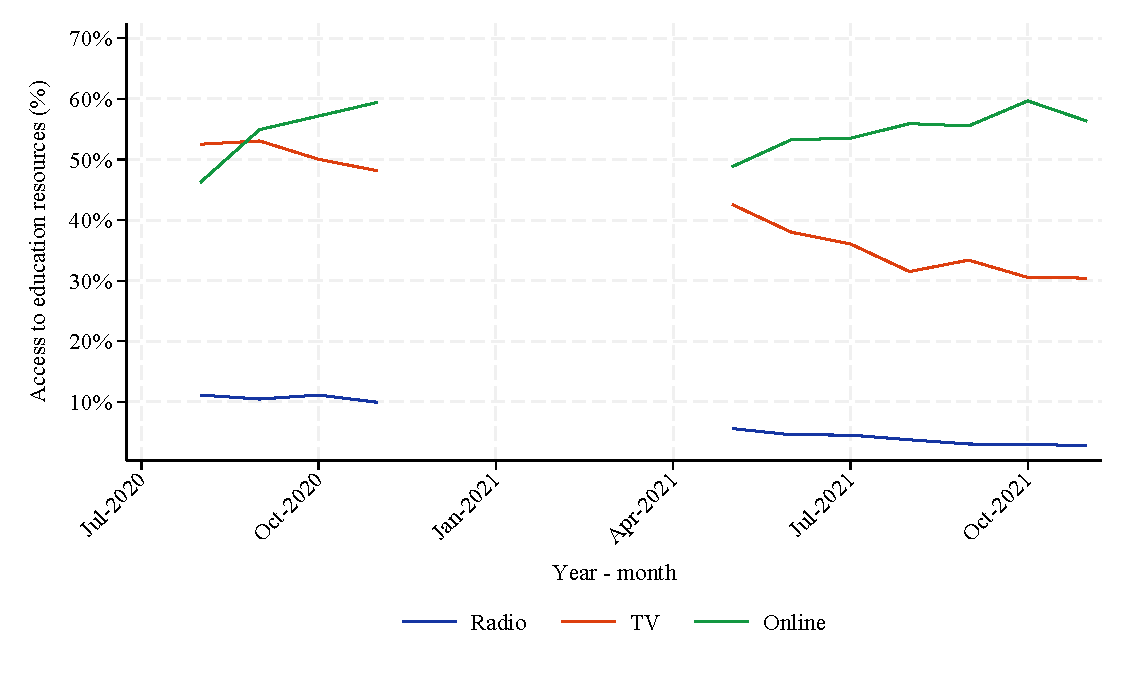
\includegraphics[width=\textwidth]{./FIGURES/Descriptive/SER_access_elm.pdf}    
    
\end{frame}

\againframe<2>{learning_home}


\begin{frame}
    \label{frame:parental_support}
    \frametitle{Parents accompany students while they attend classes and review students' work}
               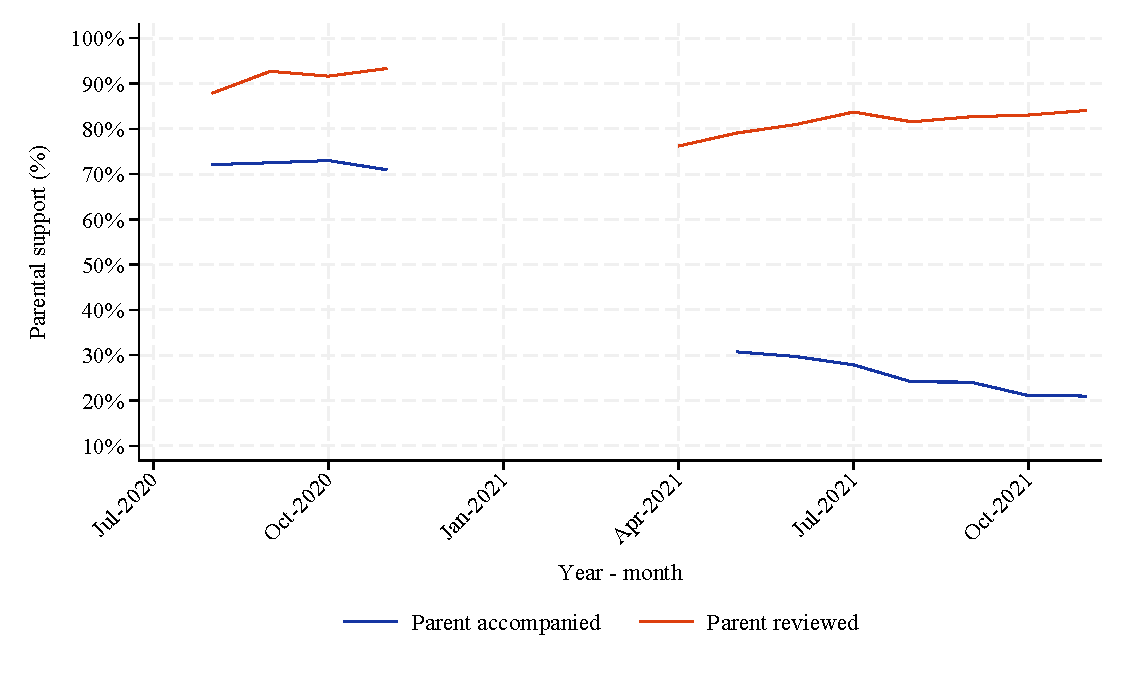
\includegraphics[width=\textwidth]{./FIGURES/Descriptive/SER_parent_elm.pdf}    
    
\end{frame}

\againframe<3>{learning_home}

\begin{frame}
    \label{frame:teacher_com}
    \frametitle{Teachers are in constant communication with parents. On average twice a week.}
               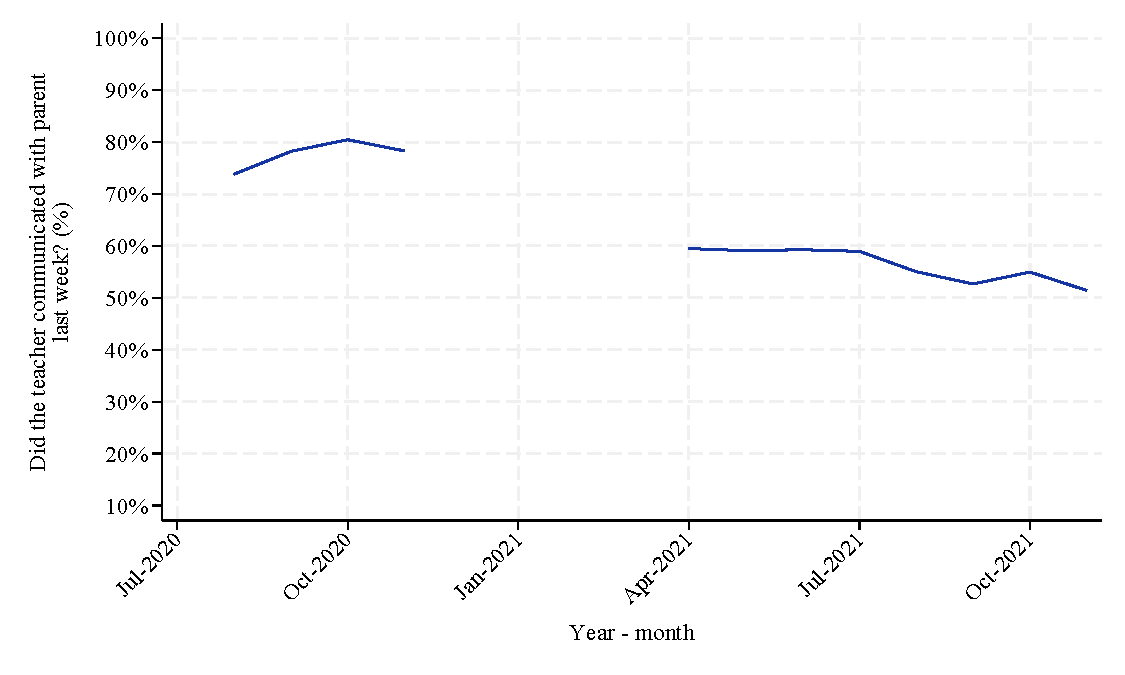
\includegraphics[width=\textwidth]{./FIGURES/Descriptive/SER_teacher_com_elm.pdf}    
    
\end{frame}





% ========================================
% DATA
% ========================================
\begin{frame}
    
    \label{frame:data}
    \frametitle{Data: Administrative (2014-2024) matched with survey}

    \begin{itemize}
        \item School progression (GPA per grade-year). 
        \begin{itemize}
            \item Teachers decide whether to promote a student to the next grade based on their assessments of competencies.
            \item Grade criteria changed during 2020-2021. Automatic grade promotion. No grade if no evidence (dropout risk).
        \end{itemize}
        \item \textcolor{blue}{Identify siblings} through matched parent's anonymized ID.
        \item Standardized test scores in 2nd, 4th, 8th grade in some years. 
        \begin{itemize}
            \item Low stakes, not used by teachers. Comparable across schools and time.
        \end{itemize}
        \item Family, student, teachers and principals surveys:
        \begin{itemize}
            \item Parental involvement in children's education
            \item Household resources and socioeconomic status
            \item Aspirations for higher education: parents (2nd and 4th grade) and students (8th grade)
            %\item Gender beliefs: "Boys are better at Math than girls"
            %\item Parental involvement: my parents ask me about my grades, I talk to my parents about what I read, why they chose school, gender beliefs, overall knowledge about school/child, etc
            %\item studying habits, beliefs, etc
            %\item Specifically related to siblings: ``Read out loud to my siblings''.
        \end{itemize}
        \item Family and teacher monitoring surveys during school closures
        %\item In both primary and secondary schools, teachers decide whether to promote a student to the next grade based on their assessments of competencies in the national curriculum (MINEDU, 2005). The national standardized examinations are not used by teachers in the decision to promote students to the next grade since the results from these examinations are only available to teachers in the following academic year by which time the promotion decision has already been made.
    \end{itemize}
\end{frame}


\begin{frame}[T]
    \label{frame:descriptive}
    \frametitle{Descriptive statistics}
    \makeatletter
\@ifclassloaded{beamer}{%
       \centering
       \resizebox{0.6\textwidth}{!}%
}{%
       \begin{table}[!tbp]\centering\def\sym#1{\ifmmode^{#1}\else\(^{#1}\)\fi}
       \centering
       \caption{Descriptive Statistics}
       \label{tab:descriptive}
       \resizebox{0.8\textwidth}{!}%
}
{
\makeatother
\begin{tabular}{lcccc}
\toprule
& Only children & 1 sibling & 2 siblings & 3 siblings  \\
\cmidrule(lr){2-2} \cmidrule(lr){3-3} \cmidrule(lr){4-4} \cmidrule(lr){5-5}
& (1) & (2) & (3) & (4)\\
\bottomrule
&  &  &  & \\
            &            &            &            &            \\
\% of sample &       0.570&       0.271&       0.122&       0.037\\
&  &  &   \\
\multicolumn{4}{l}{\textit{Panel A: School and student characteristics}} \\
            &            &            &            &            \\
\% Urban    &       0.773&       0.800&       0.741&       0.621\\
\% Public School&       0.657&       0.660&       0.749&       0.852\\
%Average Grade&       2.000&       2.000&       2.000&       2.000\\
%\% Male     &       0.513&       0.514&       0.511&       0.514\\
&  &  &   \\
\multicolumn{4}{l}{\textit{Panel B: Academic characteristics}} \\
            &            &            &            &            \\
\% Grade promotion&       0.931&       0.952&       0.934&       0.897\\
%\% Grade promotion without recovery&       0.878&       0.903&       0.884&       0.848\\
Standardized GPA - Mathematics &       0.025&       0.097&       0.030&      -0.061\\
Standardized GPA - Reading &       0.030&       0.099&       0.032&      -0.060\\
Standardized Exam - Mathematics&       0.883&       0.995&       0.883&       0.676\\
Standardized Exam - Reading&       0.930&       0.997&       0.872&       0.661\\
Did 3 years of Pre-K&       0.656&       0.665&       0.640&       0.566\\
%Has repeated a grade&       0.043&       0.033&       0.044&       0.071\\
&  &  &   \\
\multicolumn{4}{l}{\textit{Panel C: Parent's characteristics}} \\
            &            &            &            &            \\
\% Lives with both parents&       0.583&       0.649&       0.618&       0.575\\
%\% Lives with one parent&       0.197&       0.184&       0.189&       0.193\\
%\% Lives with Mother&       0.807&       0.821&       0.798&       0.764\\
%\% Lives with Father&       0.698&       0.740&       0.719&       0.687\\
%\% Father without complete secondary&       0.324&       0.278&       0.348&       0.480\\
%\% Father with complete secondary&       0.416&       0.438&       0.436&       0.391\\
%\% Father with some level of higher ed.&       0.259&       0.284&       0.215&       0.129\\
%\% Mother without complete secondary&       0.368&       0.331&       0.413&       0.563\\
\% Mother with complete secondary&       0.395&       0.418&       0.408&       0.346\\
%\% Mother with some level of higher ed.&       0.237&       0.251&       0.178&       0.090\\
&  &  &   \\
\multicolumn{4}{l}{\textit{Panel D: Household Resources (2nd grade: 2015, 2016)}} \\
            &            &            &            &            \\
Socio-Economic Index         &       0.102&       0.065&      -0.130&      -0.394\\
%HH size     &       5.007&       5.058&       5.399&       5.847\\
%\# of bedrooms&       2.853&       2.673&       2.613&       2.672\\
%\% Radio    &       0.831&       0.822&       0.789&       0.758\\
\% Internet &       0.334&       0.300&       0.234&       0.149\\
\% PC       &       0.345&       0.317&       0.243&       0.160\\
%\% Laptop   &       0.308&       0.284&       0.219&       0.141\\
\% 6+ books &       0.567&       0.521&       0.450&       0.370\\
\% Quiet room to study&       0.859&       0.854&       0.827&       0.794\\
&  &  &   \\
\multicolumn{4}{l}{\textit{Panel F: Parent's Characteristics (2nd grade: 2015, 2016)}} \\
            &            &            &            &            \\
%\% Mother with complete secondary&       0.245&       0.273&       0.276&       0.261\\
%\% Mother with some level of higher ed&       0.375&       0.397&       0.309&       0.192\\
\% Spanish  &       0.866&       0.862&       0.847&       0.829\\
%\%Education expectation: High School&       0.096&       0.080&       0.105&       0.163\\
\%Education expectation: 4-year college&       0.791&       0.817&       0.765&       0.668\\

\bottomrule
\end{tabular}
}
\@ifclassloaded{beamer}{%
}{%
       \end{table}
}

    
    % Box 1 appears on slide 2
    \only<2>{
    \highlightboxflex{-0.2}{-1.25}{1.55}{2.5}{draw=blue, draw opacity=0.8, dashed, fill=yellow!30, fill opacity=0.3}
    }
    
    % Box 3 appears on slide 3
    \only<3>{
    \highlightboxflex{1.4}{-1.25}{0.85}{2.5}{draw=blue, draw opacity=0.8, dashed, fill=yellow!30, fill opacity=0.3}
    }
    
    % Box 4 appears on slide 4
    \only<4>{
    \highlightboxflex{2.25}{-1.25}{0.85}{2.5}{draw=blue, draw opacity=0.8, dashed, fill=yellow!30, fill opacity=0.3}
    }
    
    % Box D appears on slide 5
    \only<5>{
    \highlightboxflex{-0.2}{-3}{3.2}{1.35}{draw=red, draw opacity=0.8, dashed, fill=green!30, fill opacity=0.3}
    }
    
    \begin{tikzpicture}[overlay, remember picture]
         % Single text label at the bottom
        %\node[red, above] at ([shift={(0,-4.5)}]current page.center) {\small Larger learning losses when children have siblings!};
        
        % Box 1 arrow and text (appears on slide 2)
        \only<2>{
        %\draw[->, thick, blue, opacity=0.8] ([shift={(1.35,1)}]current page.center) -- ([shift={(3,1)}]current page.center);
        \node[blue, right] at ([shift={(3.05,1)}]current page.center) {\small Children with one \\ sibling perform \\ slightly higher};
        }
        
        % Box 3 arrow and text (appears on slide 3)
        \only<3>{
        %\draw[->, thick, blue, opacity=0.8] ([shift={(2.55,0)}]current page.center) -- ([shift={(3,0)}]current page.center);
        \node[blue, right] at ([shift={(3.05,0)}]current page.center) {\small Children with two \\ sibling perform \\ similarly};
        }
        
        % Box 4 arrow and text (appears on slide 4)
        \only<4>{
        %\draw[->, thick, blue, opacity=0.8] ([shift={(3.1,-1)}]current page.center) -- ([shift={(3,-1)}]current page.center);
        \node[blue, right] at ([shift={(3.05,-1)}]current page.center) {\small Children with two \\ sibling perform \\ slighly lower};
        }
        
        % Box D arrow and text (appears on slide 5)
        \only<5>{
        %\draw[->, thick, red, opacity=0.8] ([shift={(3.0,-2.33)}]current page.center) -- ([shift={(3.45,-2.33)}]current page.center);
        \node[red, right] at ([shift={(3.0,-2.33)}]current page.center) {\small Access to resources \\ is similar for first  \\ two groups but \\ lower for next two};
        }
    \end{tikzpicture}
\end{frame}

% ========================================
% DATA
% ========================================
\begin{frame}
    \label{frame:ece_trends}
    \frametitle{Learning losses in standardized exams for both, but larger for children with siblings}
               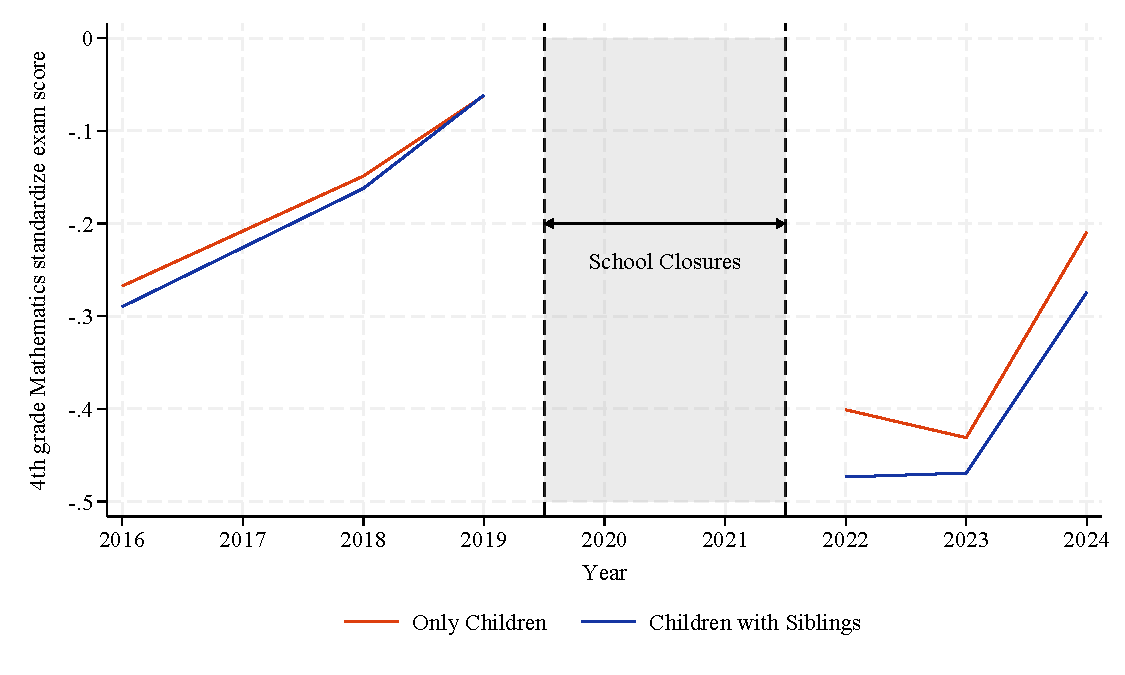
\includegraphics[width=\textwidth]{./FIGURES/Descriptive/raw_ece_math_4.pdf}    
    
\end{frame}

\begin{frame}
    \label{frame:gpa_trends}
    \frametitle{Differences in GPA also become larger}
               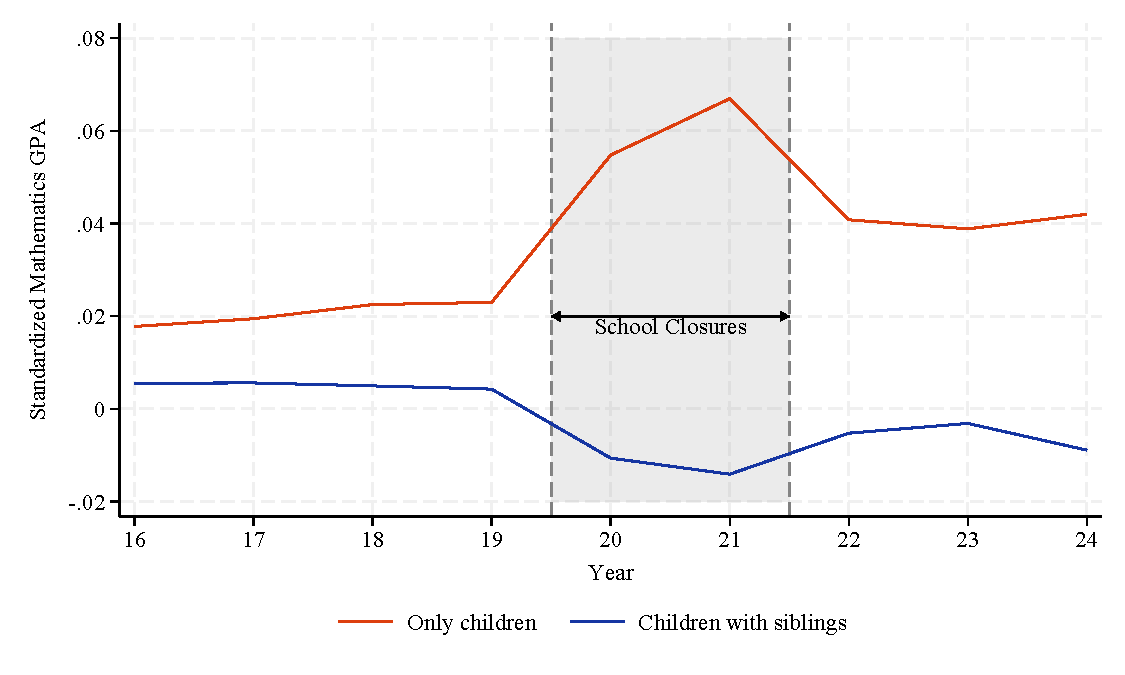
\includegraphics[width=\textwidth]{./FIGURES/Descriptive/raw_shade_total_elm_std_gpa_m_adj_Tsiblings_Sall_Size2_4.pdf}    
            \hyperlink{frame:gpa_trends_grades_elm}{\beamergotobutton{GPA trends by grade}}
  
\end{frame}


\begin{frame}
    \label{frame:pisaclosure}
    \frametitle{Change in learning gaps by duration of school closure}
    
    \begin{figure}
        \centering
        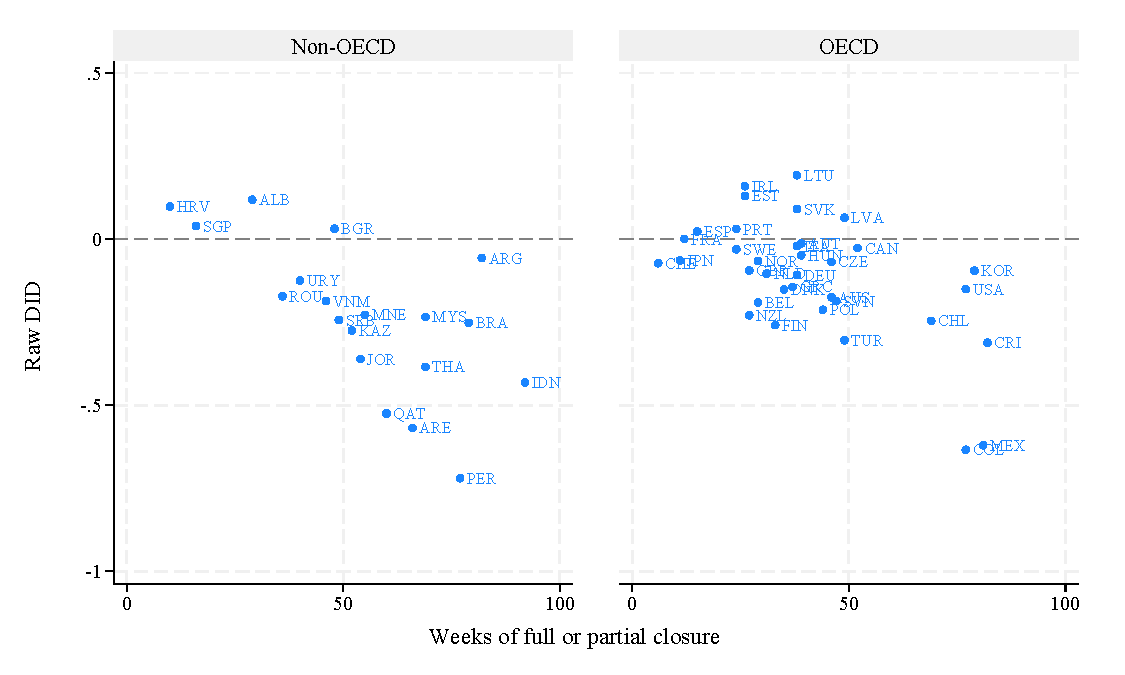
\includegraphics[width=0.9\textwidth]{./FIGURES/Descriptive/PISA_raw_DID_PV4MATH_not_fully_open.pdf}
        \caption{Similar pattern in rest of the world}
        \label{fig:1b}
    \end{figure}

    \begin{flushleft}
        \hyperlink{frame:india}{\beamergotobutton{Evidence from India}}
    \end{flushleft}  
    
    
\end{frame}


\begin{comment}
\begin{transitionframe}
    \label{frame:trends}
    \frametitle{Trends in data}
    \begin{columns}[T]
        \begin{column}{0.48\textwidth}
            \centering
            \textbf{\% of A's in Mathematics}
            \vspace{0.2cm}
            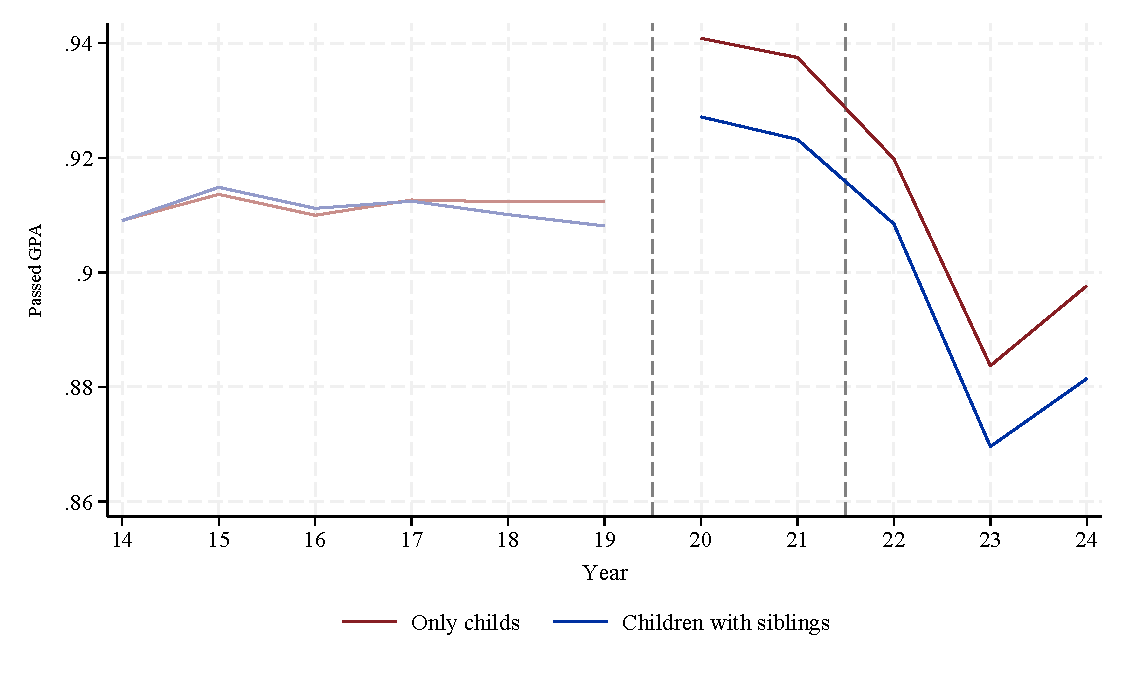
\includegraphics[width=\textwidth]{./FIGURES/Descriptive/raw_total_elm_pass_math_siblings.pdf}
        \end{column}
        \begin{column}{0.48\textwidth}
            \centering
            \textbf{Standardized GPA in Mathematics}
            \vspace{0.2cm}
            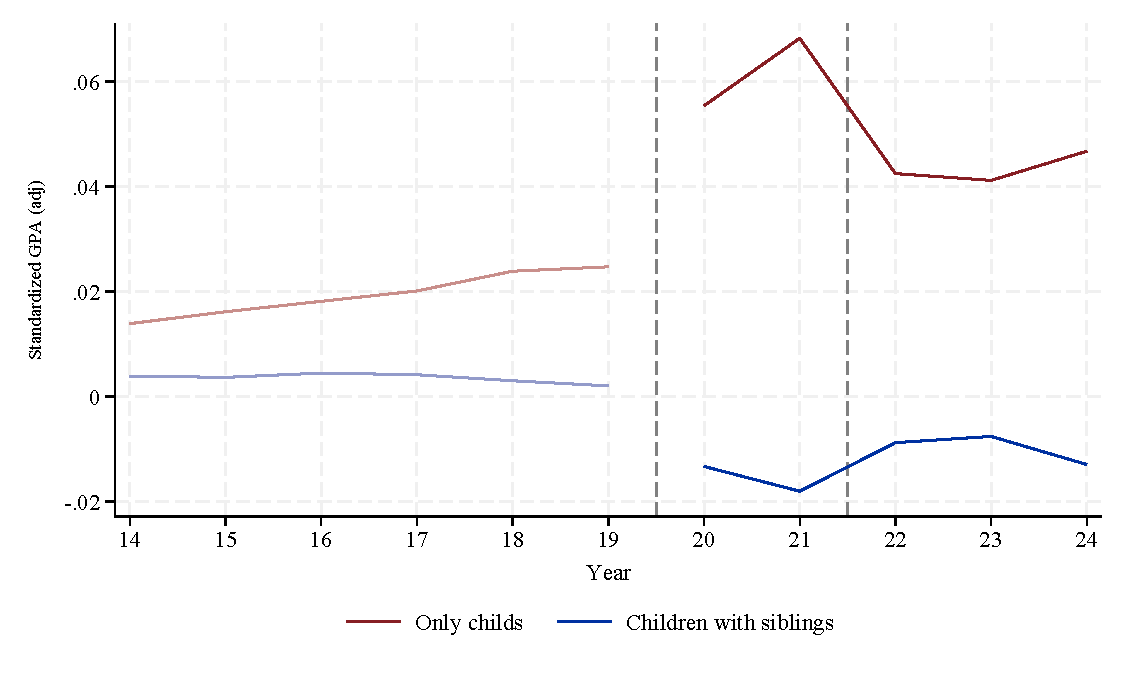
\includegraphics[width=\textwidth]{./FIGURES/Descriptive/raw_total_elm_std_gpa_m_adj_siblings.pdf}
        \end{column}
    \end{columns}
    
    
\end{transitionframe}
\end{comment}
% ========================================
% RESEARCH
% ========================================
\begin{frame}
    \label{frame:research}
    \frametitle{Research Design}
    
    \begin{block}{Identification Strategy}
    Differential changes between only children and children with siblings before and after the pandemic.
    \end{block}
    
    \begin{itemize}
         \item<2-> \textbf{No anticipation:} \\
         $\Rightarrow$ School closures were unexpected, especially if thinking about fertility
         \item<3-> \textbf{No unobserved time varying shocks:} For example, if one parent doesn't work they may choose to have \textcolor{blue}{more} or \textcolor{red}{less} children but also have more time for homeschooling $\Rightarrow$\textcolor{blue}{+}/\textcolor{red}{-}. \\
         $\Rightarrow$ Strategy controls for any unobserved time invariant shock and includes controls for potential proxies of time varying ones. I will also provide some evidence with RD and IV estimates that further address this issues.
    \end{itemize}
    
    
    %\only<3->{
    %\begin{flushleft}
    %    \hyperlink{frame:research_feedback}{\beamergotobutton{Threats}}
    %\end{flushleft}   
    %}
\end{frame}


% ========================================
% EMPIRICAL STRATEGY
% ========================================
\begin{frame}
    \label{frame:empirical}
    \frametitle{Empirical Strategy}

    
    \textbf{Difference-in-Differences Specification:}
    \small
    \begin{align}
    Y_{ist} &= \alpha + \delta_1 \text{Post}_{it} + \delta_2 \text{HasSiblings}_{i} \nonumber  \\
    &\quad + \boldsymbol{\beta} (\text{Post}_{it} \times \text{HasSiblings}_{i}) \nonumber \\
    &\quad + \mathbf{X}_{ist}'\gamma + \lambda_s + \mu_t + \varepsilon_{ist}
    \end{align}
    
    \vspace{0.1cm}
    
    \textbf{Event Study Specification:}
    \begin{align}
    Y_{ist} &= \alpha + \sum_{k=-5}^{-2} \delta_k (\mathbb{I}[t = 2020+k] \times \text{HasSiblings}_{i}) \nonumber \\
    & \quad + \sum_{k=0}^{4} \beta_k (\mathbb{I}[t = 2020 + k] \times \text{HasSiblings}_{i}) \nonumber \\
    & \quad + \mathbf{X}_{ist}'\gamma + \text{HasSiblings}_{i} + \lambda_s + \mu_t + \varepsilon_{ist}
    \end{align}
    \normalsize
    
    %where $\tau_d$ is the treatment date for district $d$, and we normalize $\beta_{-1} = \delta_{-1} = 0$.
    
\end{frame}


% ========================================
% RESULTS
% ========================================

\section{Main Results}
% A, Main Results

%A.1. Event Study (all siblings)
    %covid_event_all_all_std_gpa_m_adj_Tsiblings_Sall_4
    
%A.2. Event Study (by siblings)
    %covid_event_bysibs_all_all_std_gpa_m_adj_Tsiblings_Sall_4

% B. Mechanisms
%B.1. Birth Order
%% Double sided event and GPA bar

%B.2. Sibling rivalry
%2.1 Bar GPA by PC/internet

%2.2 Bar GPA by Age gap

%B.3. Parental time
%3.1. Descriptives about parent's
    %Who spends more time with their kids.
%3.1. By parent's

%B.4 Income
%Change in SES
%twfe_ses_2_4_8_Tsiblings_Soldest_4

% C. Other Outcomes
%C.1. Results by grade 2/4/6/8 GPA (TWFE bar plots)
    %twfe_gpa_2_4_6_8_20_21_Tsiblings_Soldest_4

%C.2. Results by grade 2/4/8 ECE
    %twfe_ece_2_4_8__Tsiblings_Sall_4

%C.3. Grade promotion
    
%C.4. College application

\begin{frame}
    \label{frame:eventstudy}
    \frametitle{A 0.04 standard deviation decline in GPA compared to only children}
        {\resizebox{0.9\textwidth}{!}{
       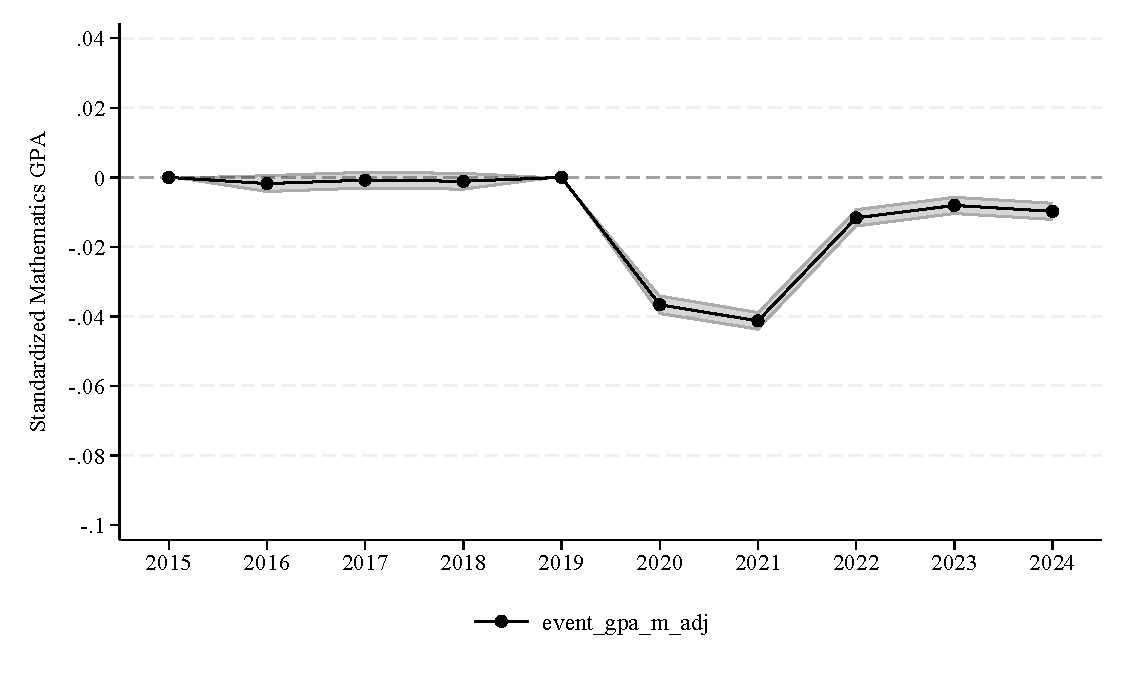
\includegraphics{./FIGURES/Event Study/covid_event_all_all_std_gpa_m_adj_Tsiblings_Sall_4.pdf}
      }
    }
\end{frame}

\begin{frame}
    \label{frame:eventstudy_bysibs}
    \frametitle{Effect is larger (and persistent) when there are more siblings}
        {\resizebox{0.9\textwidth}{!}{
       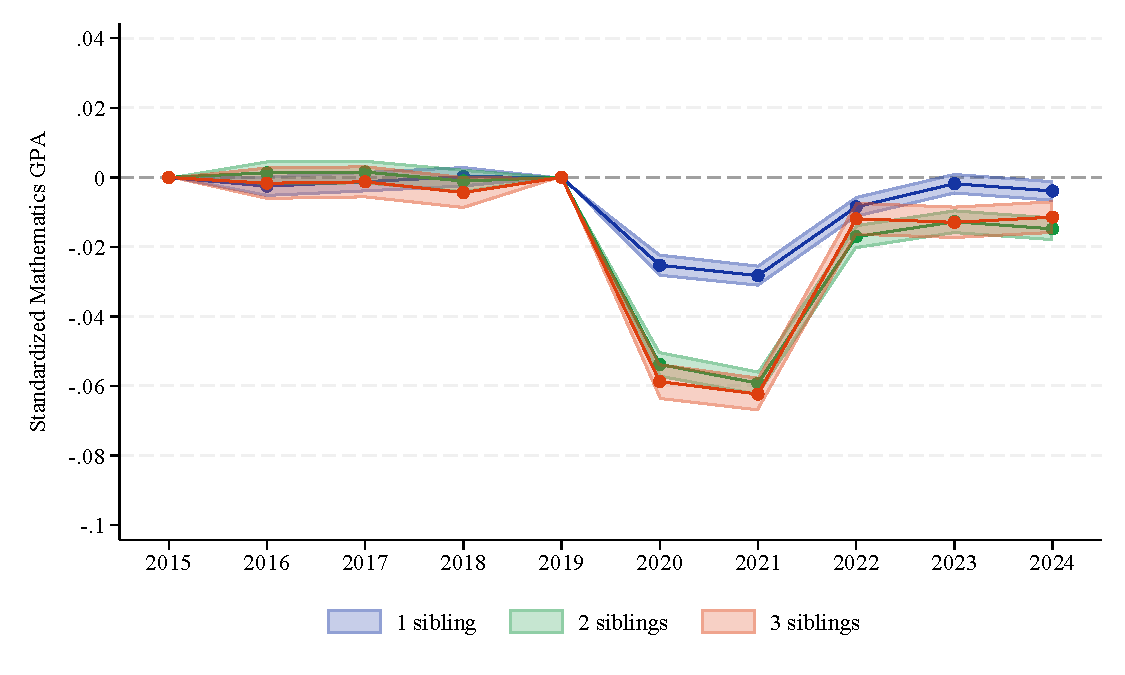
\includegraphics{./FIGURES/Event Study/covid_event_bysibs_all_all_std_gpa_m_adj_Tsiblings_Sall_4.pdf}
      }
    }
\end{frame}


\begin{frame}
        \label{frame:robustness}
        \frametitle{This happens in all type of schools \\ {\tiny TWFE for 2020-2021}}
  {\resizebox{0.9\textwidth}{!}{
    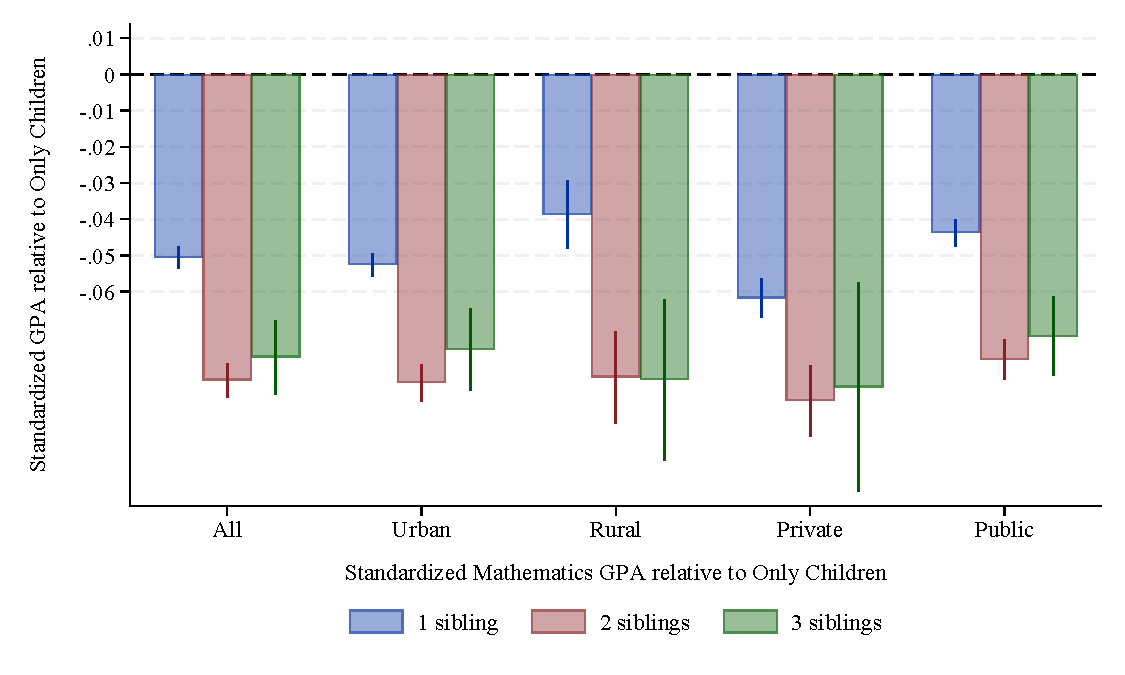
\includegraphics{./FIGURES/TWFE/covid_twfe_school_bysibs_elm_20_21_gpa_m_adj_Tsiblings_Soldest_4.pdf}
  }
}   %\input{./TABLES/MANUAL/twfe_ece_expectations.tex}
\end{frame}


\begin{frame}
    \label{frame:twfe_gpa_2_4_6_8}
    \frametitle{Effect on GPA is larger in earlier grades}
        {\resizebox{0.9\textwidth}{!}{
       %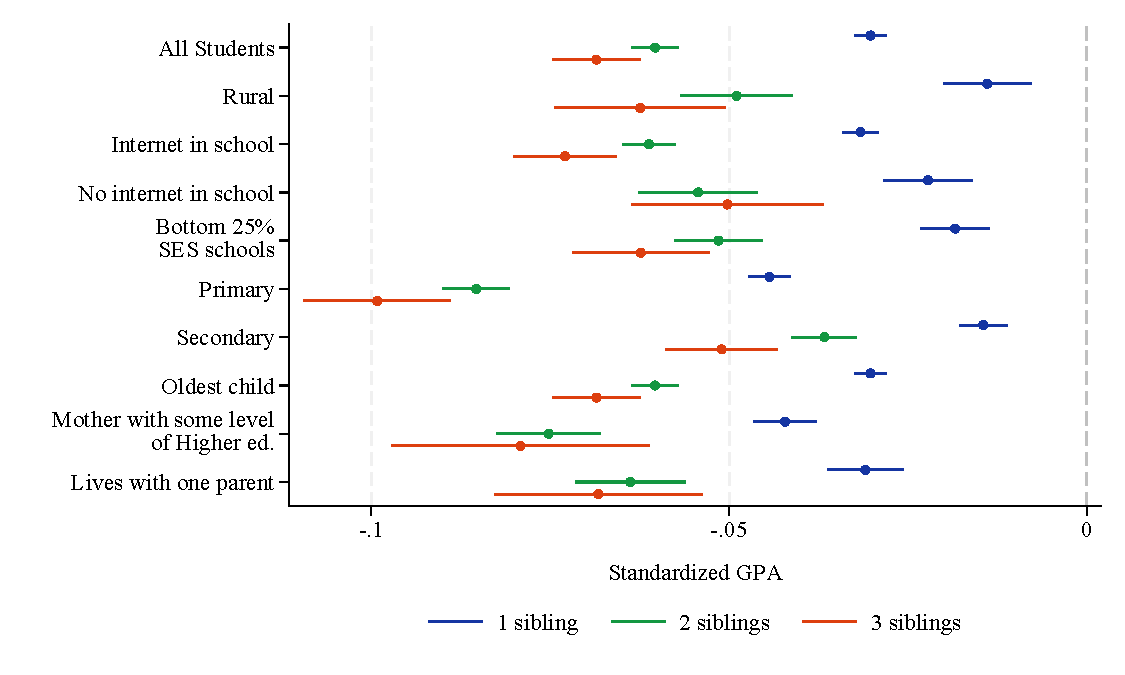
\includegraphics{./FIGURES/TWFE/covid_twfe_summ_bysibs_all_20-21_gpa_m_adj_Tsiblings_Soldest_4.pdf}
       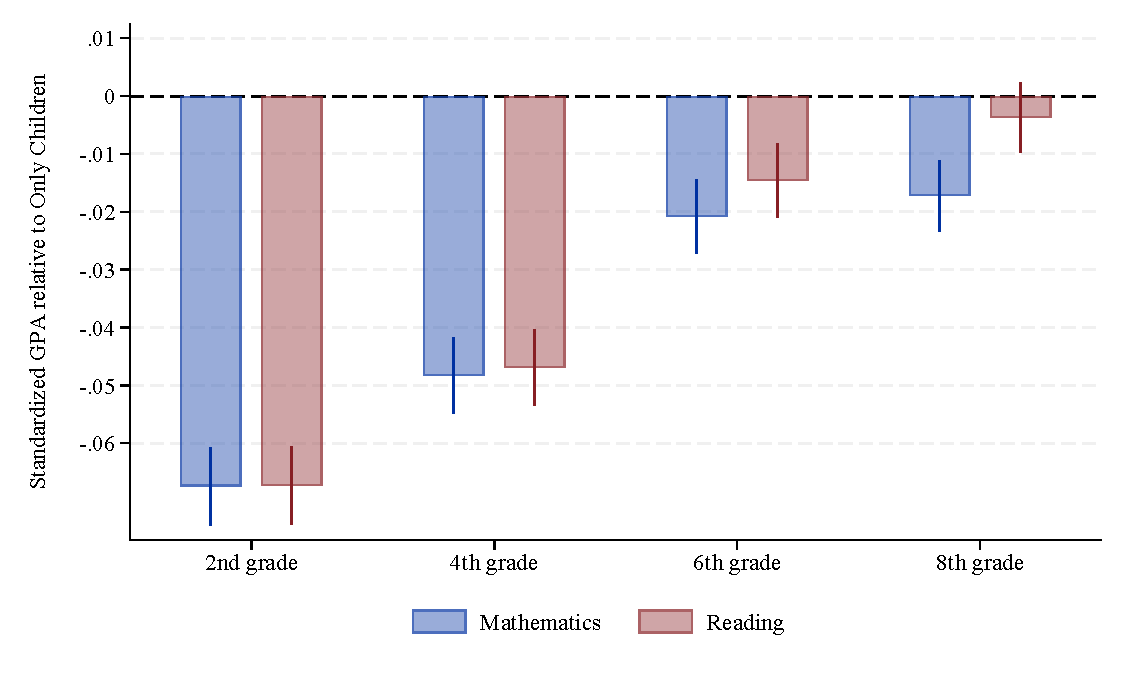
\includegraphics{./FIGURES/TWFE/twfe_gpa_2_4_6_8_20_21_Tsiblings_Soldest_4.pdf}
      }
    }
\end{frame}

\begin{frame}
    \label{frame:recap1}
    \frametitle{What about standardized exams?}
    \begin{itemize}
       \item So far we have seen that children with siblings do worse in terms of GPA.
        \begin{itemize}
            \item Worse when there are more siblings
            \item Happens in Urban/Rural and Public/Private schools
            \item Worse when they are younger
            \item Effects can be persistent
        \end{itemize}
        \item What about actual performance in standardized exams years afters school reopen?
    \end{itemize}
\end{frame}

\begin{frame}
    \label{frame:twfe_gpa_2_4_8}
    \frametitle{Similar pattern in elementary school even 3 years after schools open (2022-2024)}
        {\resizebox{0.9\textwidth}{!}{
       %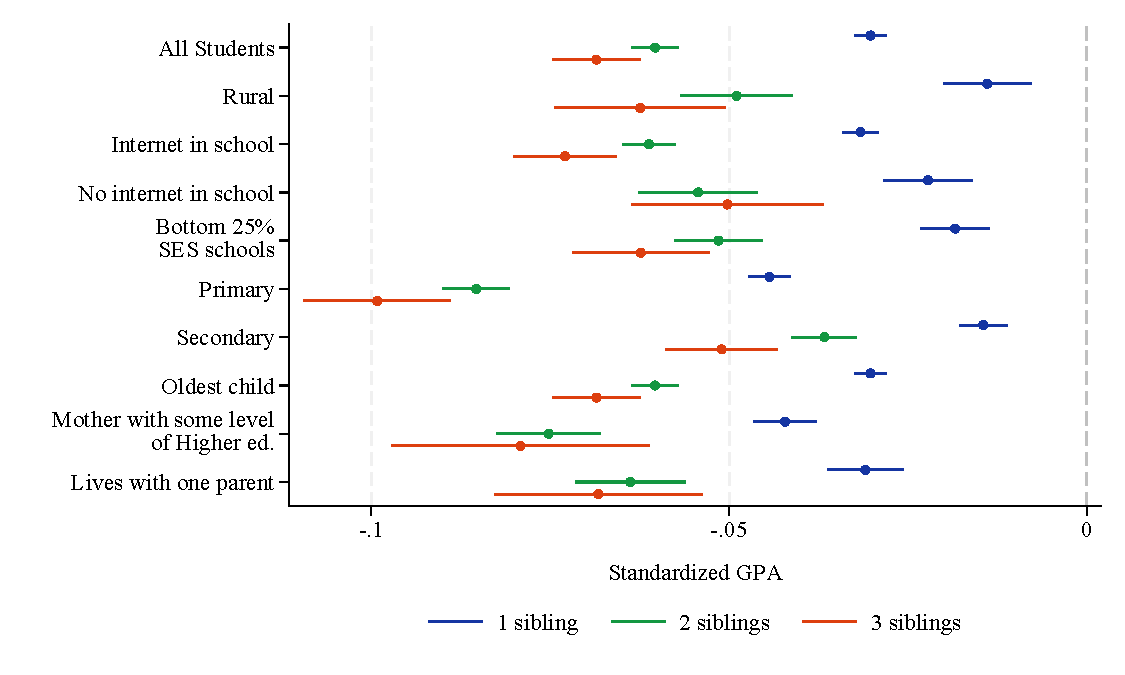
\includegraphics{./FIGURES/TWFE/covid_twfe_summ_bysibs_all_20-21_gpa_m_adj_Tsiblings_Soldest_4.pdf}
       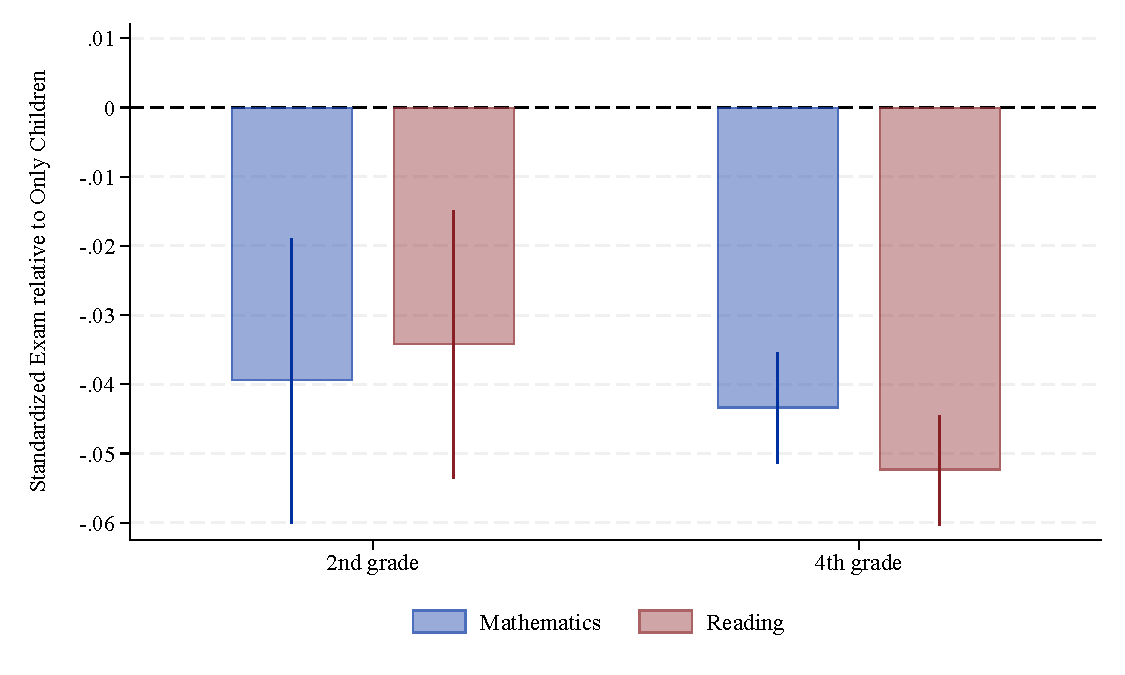
\includegraphics{./FIGURES/TWFE/twfe_ece_2_4_Tsiblings_Soldest_4.pdf}
      }
    }
\end{frame}


\begin{frame}
    \label{frame:twfe_gpa_controls_intro}
    \frametitle{Controlling for baseline scores and SES}
       \begin{itemize}
           \item Using the administrative data we can control for sex, mother's age, mother's age at first birth, mother's education, and school, year and grade FE.
           %\item In some cases, I can use survey data for a more rich set of controls.
           \item For some years, we can match students in 6th, 7th and 9th grade with baseline characteristics from 2nd, 4th and 8th grade.
           \item We could expect potential unobserved time varying differences to be correlated with SES, academic performance or parental education.
           \item However, similar results for the TWFE estimate when controlling for demographics, baseline standardized exams and socioeconomic index controls.


%    - 1. 2° (2015,2016) 					→ 6° (2019,2020)
%	- 2. 2° (2014,2016) + 4° (2016,2018) 	→ 6° (2018,2020)
%	- 3. 2° (2014,2016) + 4° (2016,2018) 	→ 7° (2019,2021)
%	- 4. 2° (2012,2013) + 8° (2018,2019) 	→ 9° (2019,2020)              
       \end{itemize}
\end{frame}


\begin{frame}
    \label{frame:twfe_gpa_controls}
    \frametitle{Results do not change when controlling for scores and socio-economic status}
        {\resizebox{0.9\textwidth}{!}{
       %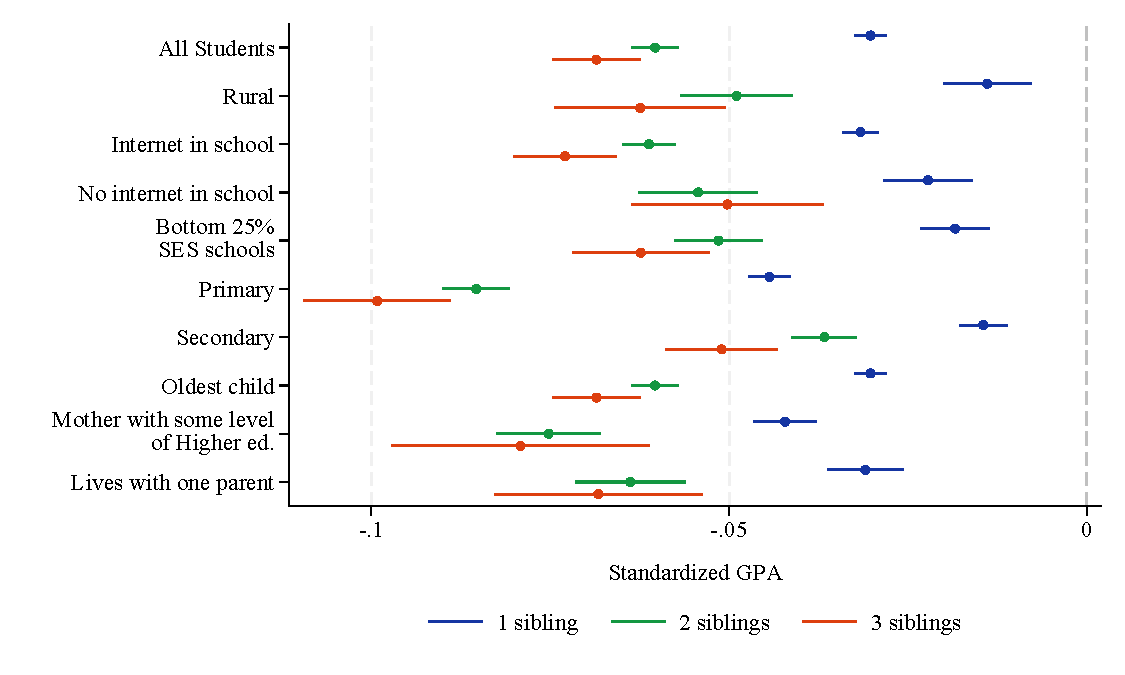
\includegraphics{./FIGURES/TWFE/covid_twfe_summ_bysibs_all_20-21_gpa_m_adj_Tsiblings_Soldest_4.pdf}
       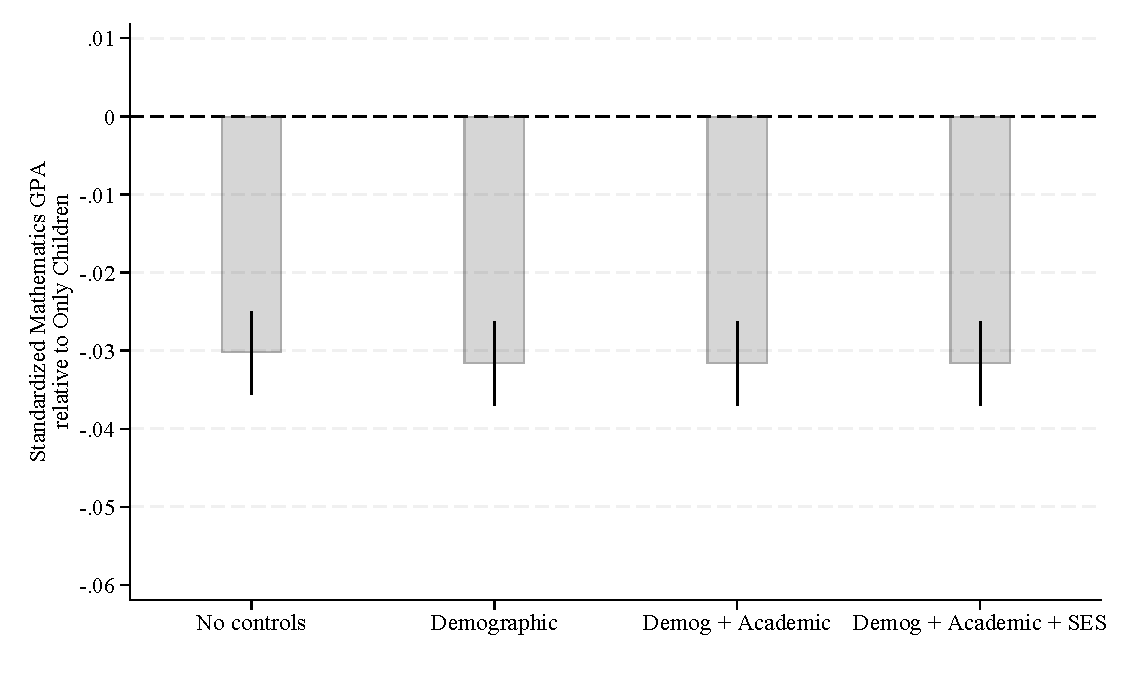
\includegraphics{./FIGURES/TWFE/twfe_std_gpa_m_adj_bycontrols_Tsiblings_Soldest_pairall_4.pdf}
      }
    }

      \begin{flushleft}
        \hyperlink{frame:twfe_gpa_controls_siblings}{\beamergotobutton{Results by siblings}}
        \hyperlink{frame:twfe_gpa_controls_1}{\beamergotobutton{6th-2nd grade}}
        \hyperlink{frame:twfe_gpa_controls_2}{\beamergotobutton{6th-4th grade}}
         \hyperlink{frame:twfe_gpa_controls_3}{\beamergotobutton{7th-4th grade}}
        \hyperlink{frame:twfe_gpa_controls_4}{\beamergotobutton{9th-8th grade}}  
    \end{flushleft}     
\end{frame}

\begin{frame}
    \label{frame:twfe_gpa_controls_siblings}
    \frametitle{And similar pattern when looking at effects by siblings}
        {\resizebox{0.9\textwidth}{!}{
        %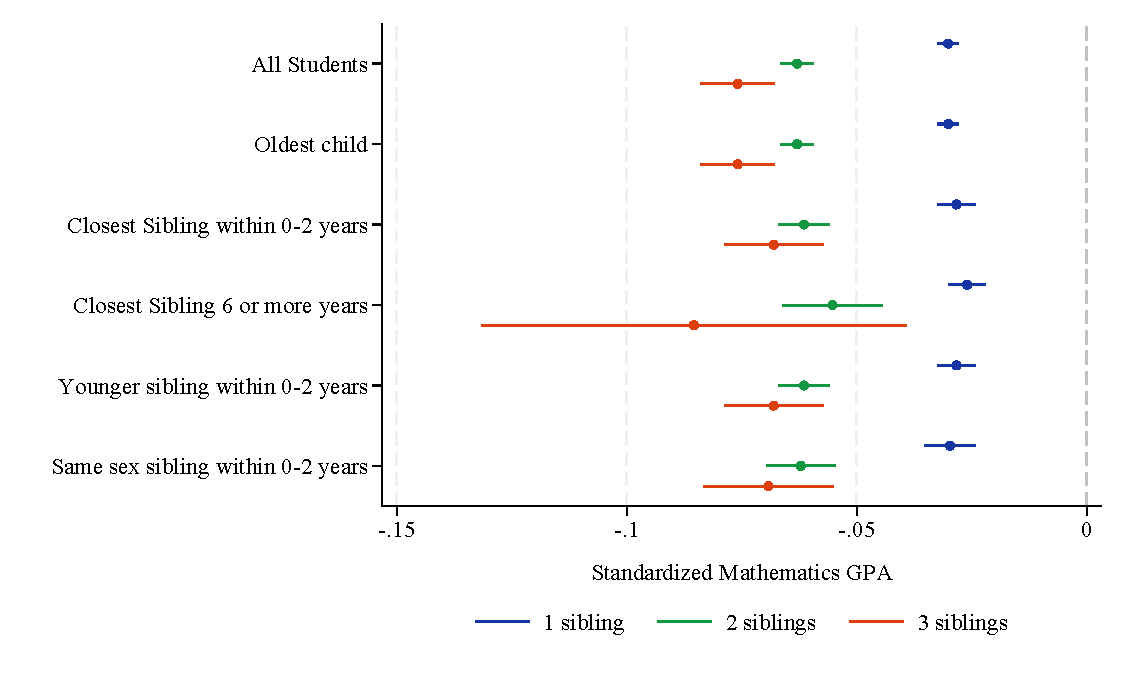
\includegraphics{./FIGURES/TWFE/covid_twfe_C_bysibs_elm_all_gpa_m_adj_Tsiblings_Soldest_4.pdf}
       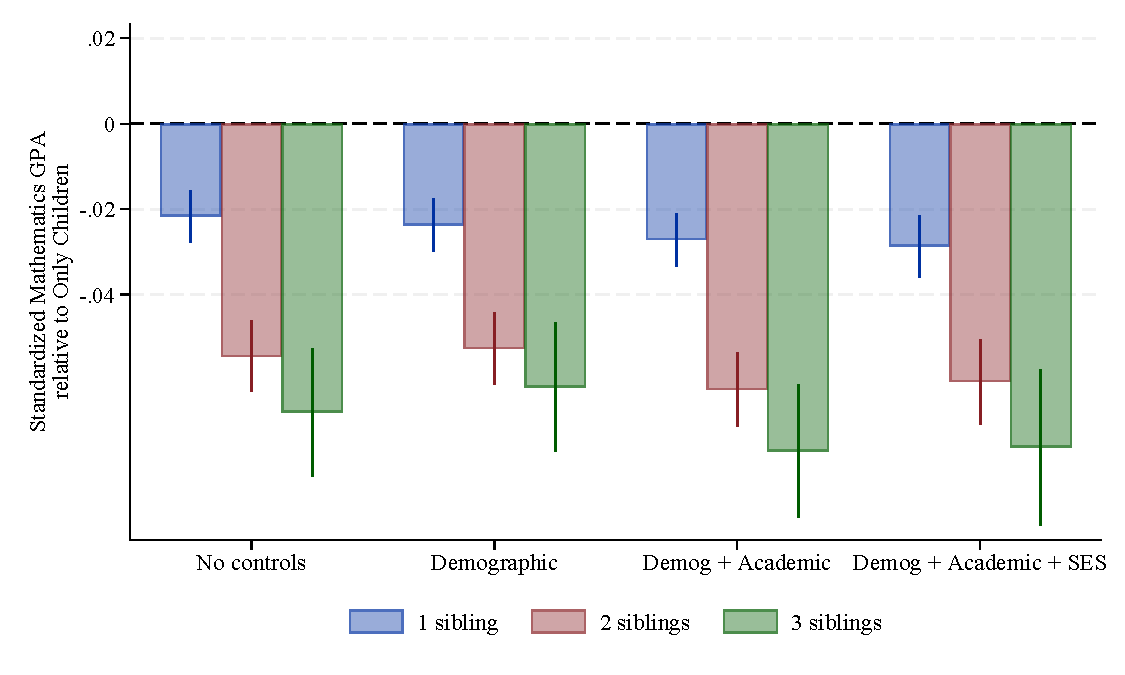
\includegraphics{./FIGURES/TWFE/twfe_std_gpa_m_adj_bycontrols_bysibs_Tsiblings_Soldest_pairall_4.pdf}
      }
    }

    \begin{flushleft}
        \hyperlink{frame:twfe_gpa_controls}{\beamergotobutton{Go Back $\carriagereturn$}}
    \end{flushleft}       

\end{frame}



% ========================================
% MECHANISMS
% ========================================
\begin{frame}<1-2>
    [label=mechanisms]
    \frametitle{Why do children with siblings do worse than only children?}
\begin{itemize}
    \item Having a sibling is related with larger learning losses.
    \item School closures and lockdowns can make students interact less with teachers and peers and more with parents and siblings.
    \item Potential Mechanisms:   
    \begin{itemize}
        \item \only<1,2>{\color{black}}\only<3-6>{\color{gray!30}}Birth Order
        \item \only<1,3>{\color{black}}\only<2,4-6>{\color{gray!30}}Scarce material resources
        \item \only<1,4>{\color{black}}\only<2-3,5-6>{\color{gray!30}}Sibling disruption
        \item \only<1,5>{\color{black}}\only<2-4,6>{\color{gray!30}}Parental resources
        \item \only<1,6>{\color{black}}\only<2-5>{\color{gray!30}}Income Shocks
    \end{itemize} 
\end{itemize}
\end{frame}

\begin{frame}
    \label{frame:birthorder}
    \frametitle{Separating birth order from family size effects}
       \begin{itemize}
           \item Effects from school closures may be different for the 1st, 2nd, 3rd... children.
           \item This is different from family size effects.
           \item In order to separate both, we only consider first-born children.
       \end{itemize}
\end{frame}

\begin{frame}
    \label{frame:birthorder_intro}
    \frametitle{Similar results with first-born children}
        {\resizebox{0.9\textwidth}{!}{ 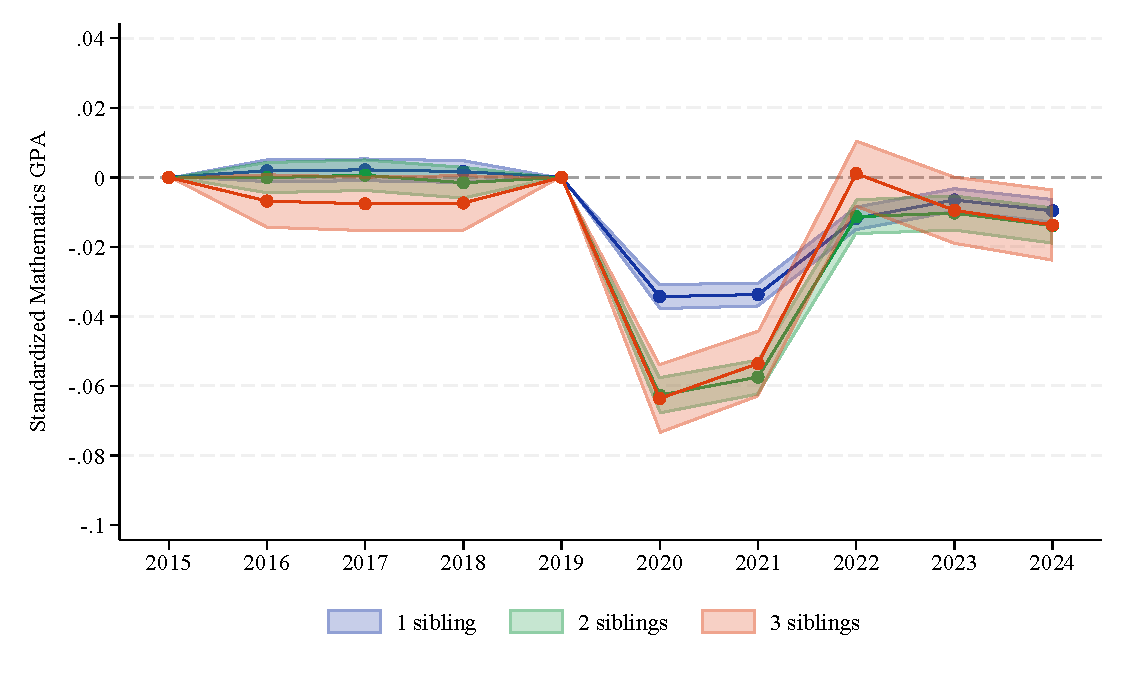
\includegraphics{./FIGURES/Event Study/covid_event_bysibs_all_all_std_gpa_m_adj_Tsiblings_Soldest_4.pdf}
      }
    }  

    \begin{flushleft}
        \hyperlink{frame:mechanisms}{\beamergotobutton{Mechanisms}}
    \end{flushleft}
\end{frame}

% Show overlay 3 (Birth Order highlighted)
\againframe<3>{mechanisms}

\begin{frame}
    \label{frame:resources_intro}
    \frametitle{Siblings may compete for access to phone, TV, radio or computer}
       \begin{itemize}
           \item Siblings may be competing for access to school resources, do homework and send materials. They might also need it for leisure.
           \item But households with less resources show similar patterns 
       \end{itemize}
\end{frame}

\begin{frame}
    \label{frame:resources}
    \frametitle{Similar effects by access to resources}
        {\resizebox{0.9\textwidth}{!}{
        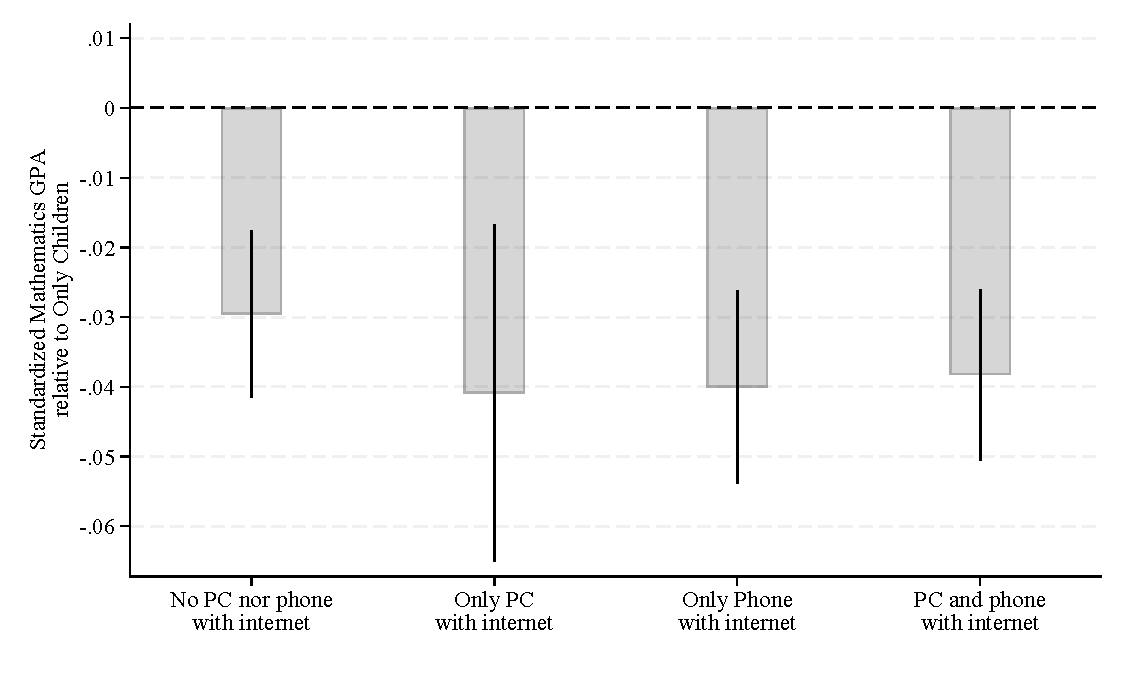
\includegraphics{./FIGURES/TWFE/twfe_std_gpa_m_adj_byresour4_Tsiblings_Soldest_pairall_4.pdf}
      }
    }

    \begin{flushleft}
        \hyperlink{frame:resources_siblings}{\beamergotobutton{Results by siblings}}
    \end{flushleft}    

\end{frame}





% Show overlay 4 (Scarce material resources highlighted)  
\againframe<4>{mechanisms}

\begin{frame}
    \label{frame:siblingdisruption_intro}
    \frametitle{Siblings may also be disrupting or distracting each other}
       \begin{itemize}
           \item Having to study at home also means having your sibling nearby. 
           \item Distracting siblings may impact students negatively
           \item Siblings close in age are more likely to interact with each other
           \item However, I don't see big differences between siblings who are 0-2 and 3-5 years appart. 
           \item \textcolor{green}{6+ show a smaller effect which made me think about how this may also be confounding parental inputs because older siblings require less from parents. Might need a different approach to it}
       \end{itemize}
\end{frame}


\begin{frame}
    \label{frame:siblingdisruption}
    \frametitle{Similar effects when siblings are 0-2 and 3-5 years apart}
        {\resizebox{0.9\textwidth}{!}{
        %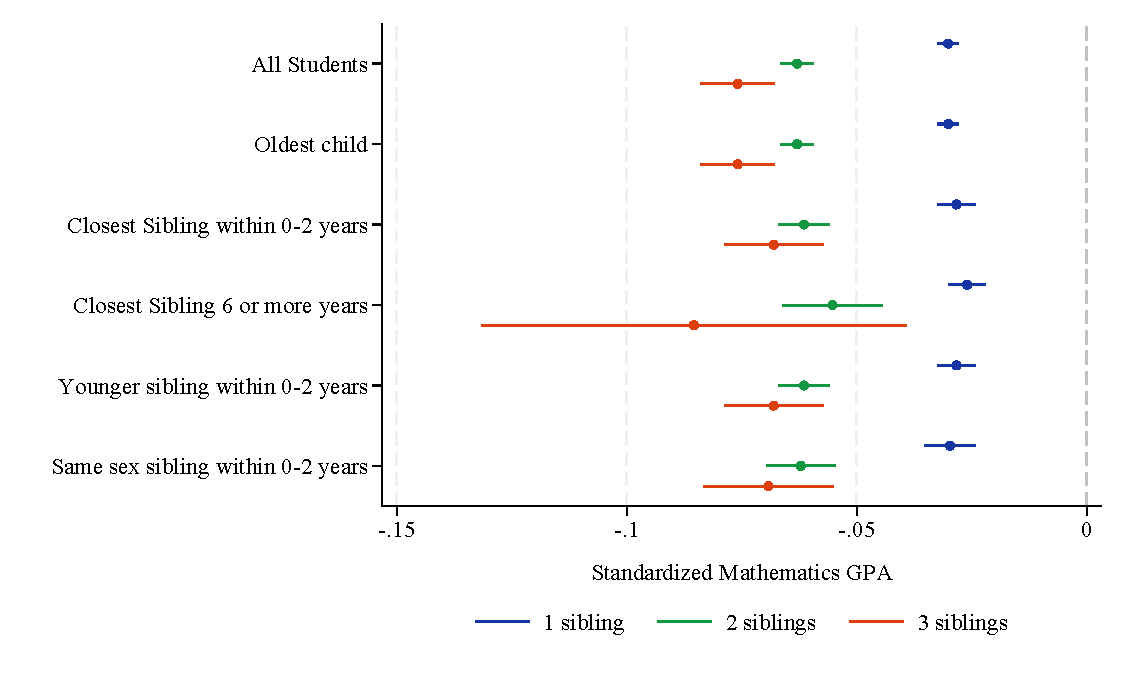
\includegraphics{./FIGURES/TWFE/covid_twfe_C_bysibs_elm_all_gpa_m_adj_Tsiblings_Soldest_4.pdf}
        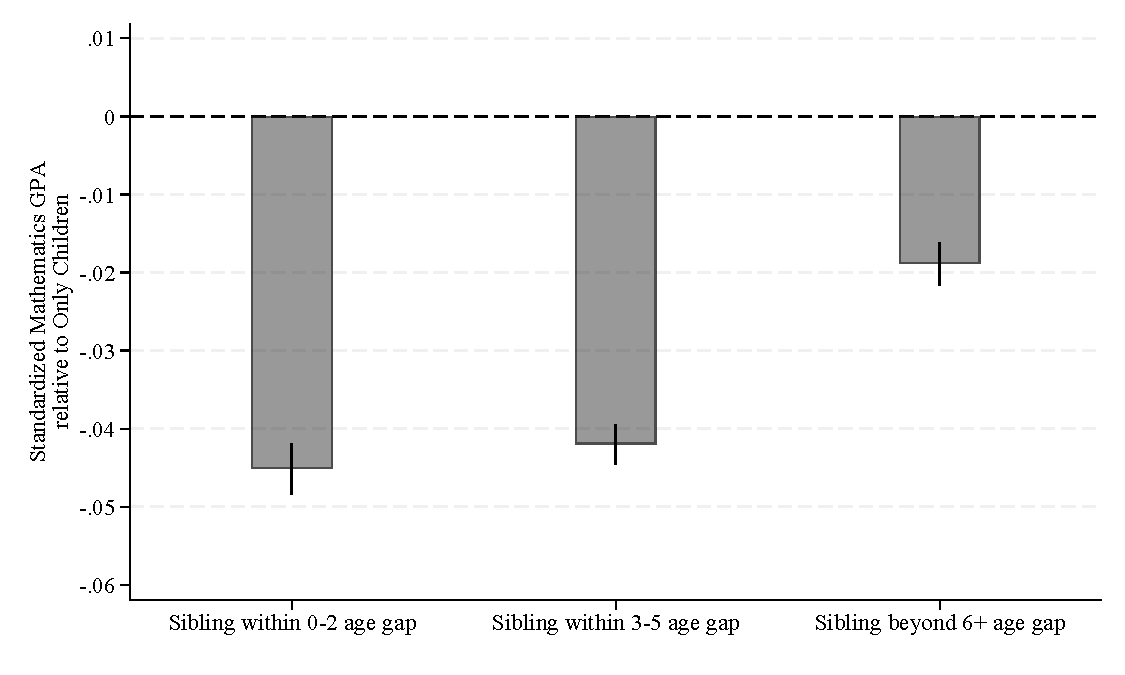
\includegraphics{./FIGURES/TWFE/twfe_gpa_age_gap_20_21_Tsiblings_Soldest_4.pdf}
      }
    }

    \begin{flushleft}
        \hyperlink{frame:siblingdisruption_siblings}{\beamergotobutton{Results by siblings}}
    \end{flushleft}    

\end{frame}



% Show overlay 5 (Sibling disruption highlighted)
\againframe<5>{mechanisms}

\begin{frame}
    \label{frame:parentaldilution_intro}
    \frametitle{Do parents struggle to keep up with more children?}
       \begin{itemize}
           \item Parent's loose childcare and school support.
           %\item This increhey need to take up on childcare.
           \item Parental time investment becomes more relevant and may at the same time increase.
           \item Around $50\%$ of students accessed school material in the company of their parents. Only 12\% in the company of a sibling. %[Family surveys, Ministry of Education, July 2020]


           
           %\item Additionally, they may need to provide help with schoolwork.
           \item ``Parents who before the pandemic invested time and resources in their children use official education resources the most...  \textbf{[low SES]} spent  even less time during the lockdowns.'' {\tiny\cite{naslund-hadley_education_2021}}
       \end{itemize}
\end{frame}

\begin{frame}
    \label{frame:parental_investments_vs_ses}
    \frametitle{Parental time helping with schoolwork is correlated with SES}
        {\resizebox{0.9\textwidth}{!}{
        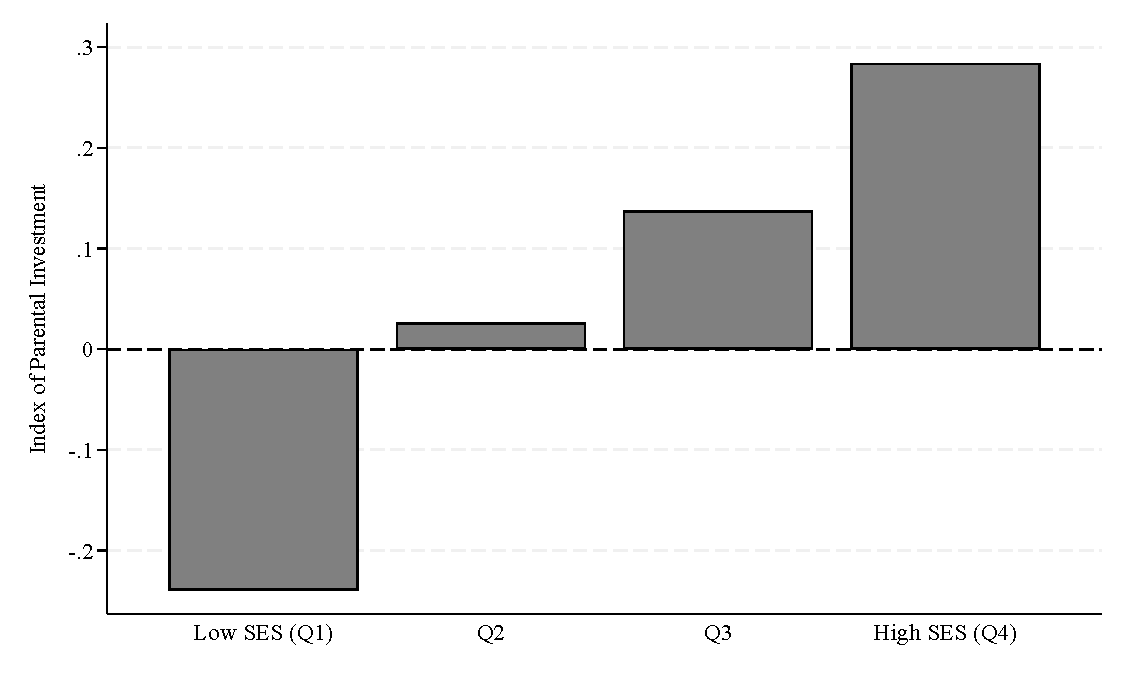
\includegraphics{./FIGURES/Descriptive/parental_investment_ses.pdf}
      }
    }

\end{frame}


\begin{frame}
    \label{frame:byses}
    \frametitle{When parent's invest little time, there are smaller size effects}
        {\resizebox{0.9\textwidth}{!}{
        %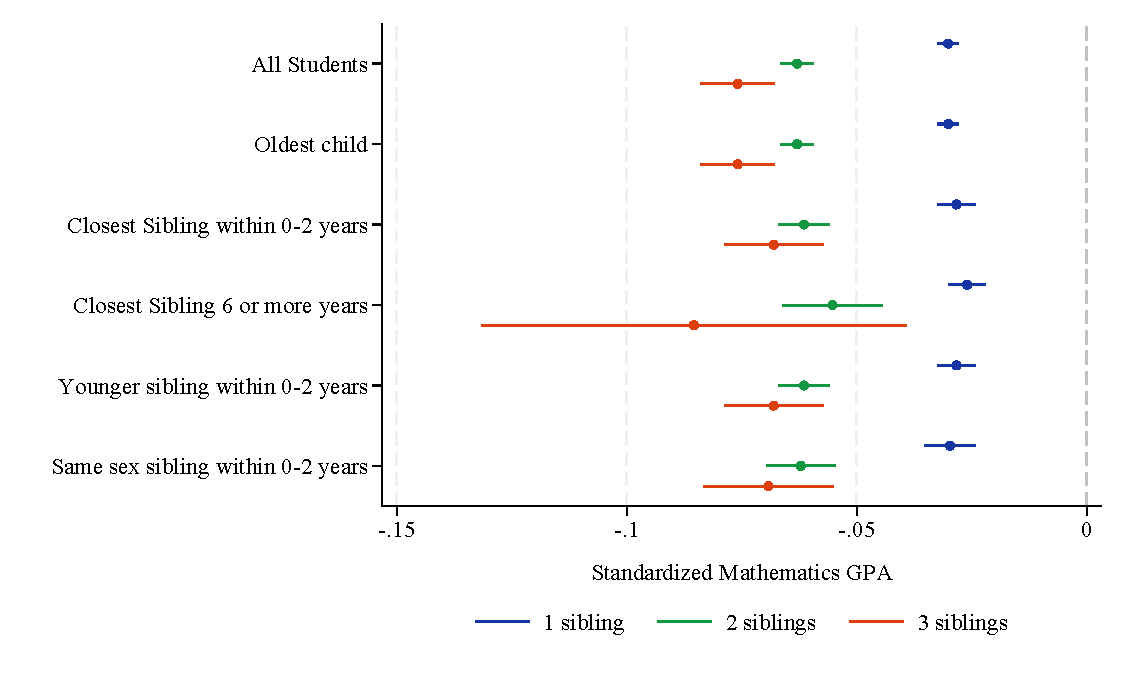
\includegraphics{./FIGURES/TWFE/covid_twfe_C_bysibs_elm_all_gpa_m_adj_Tsiblings_Soldest_4.pdf}
        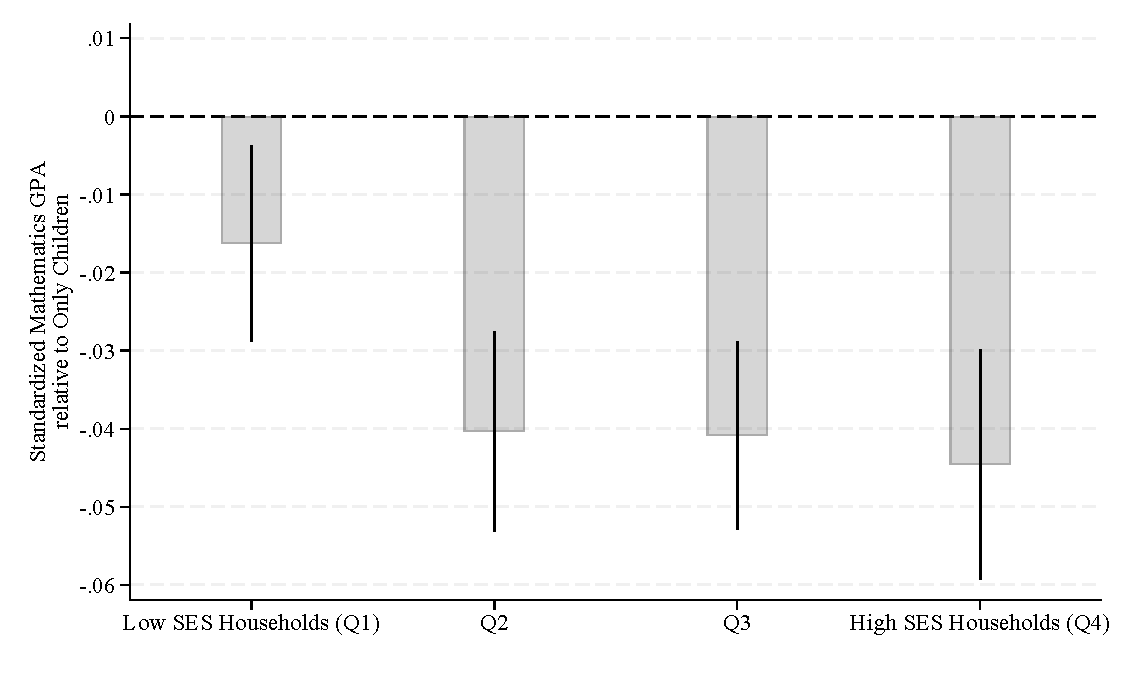
\includegraphics{./FIGURES/TWFE/twfe_std_gpa_m_adj_byses4_Tsiblings_Soldest_pairall_4.pdf}
      }
    }

    \begin{flushleft}
        \hyperlink{frame:byses_siblings}{\beamergotobutton{Results by siblings}}
    \end{flushleft}    

\end{frame}

\begin{frame}
    \label{frame:byses_siblings}
    \frametitle{Similar pattern by number of siblings}
        {\resizebox{0.9\textwidth}{!}{
        %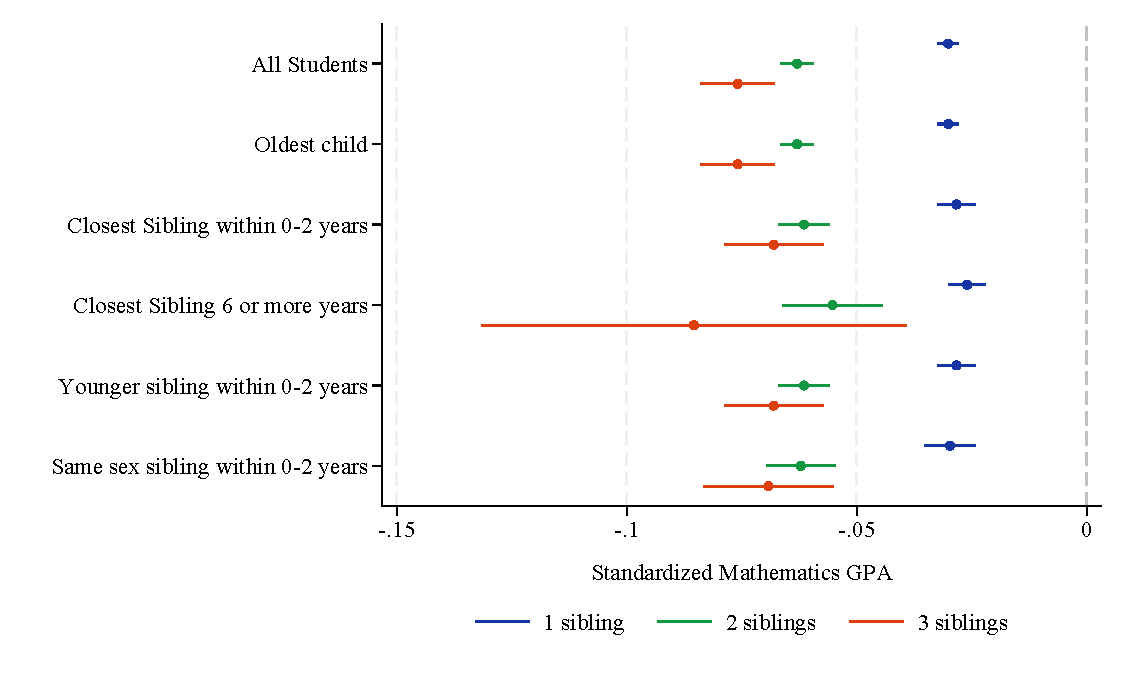
\includegraphics{./FIGURES/TWFE/covid_twfe_C_bysibs_elm_all_gpa_m_adj_Tsiblings_Soldest_4.pdf}
        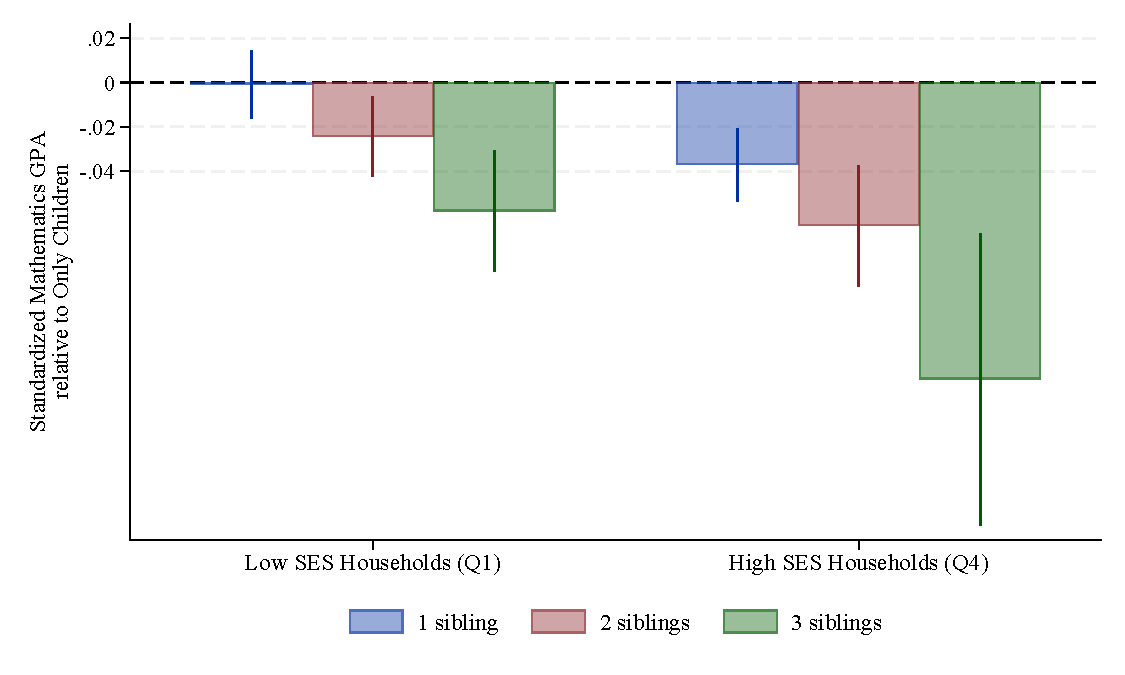
\includegraphics{./FIGURES/TWFE/twfe_std_gpa_m_adj_byses_bysibs_Tsiblings_Soldest_pairall_4.pdf}
      }
    }

    \begin{flushleft}
        \hyperlink{frame:byses}{\beamergotobutton{Go Back $\carriagereturn$}}
    \end{flushleft}        

\end{frame}




\begin{comment}
\begin{frame}
    \label{frame:livesmother}
    \frametitle{Lives with mother}
        {\resizebox{0.9\textwidth}{!}{
        %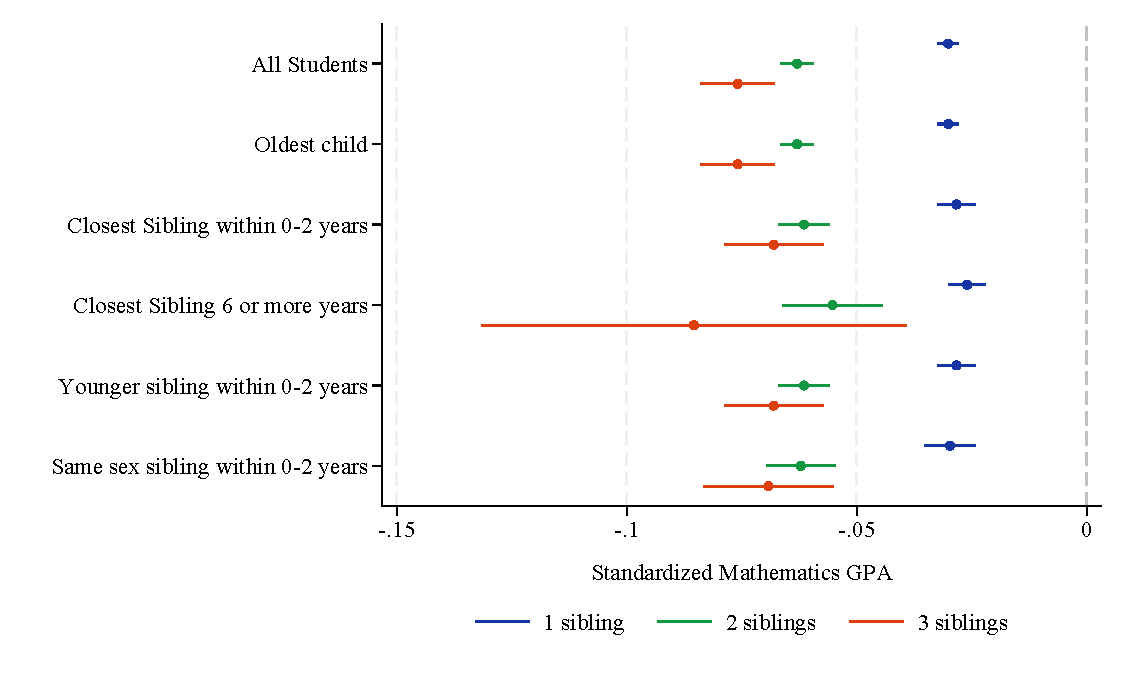
\includegraphics{./FIGURES/TWFE/covid_twfe_C_bysibs_elm_all_gpa_m_adj_Tsiblings_Soldest_4.pdf}
        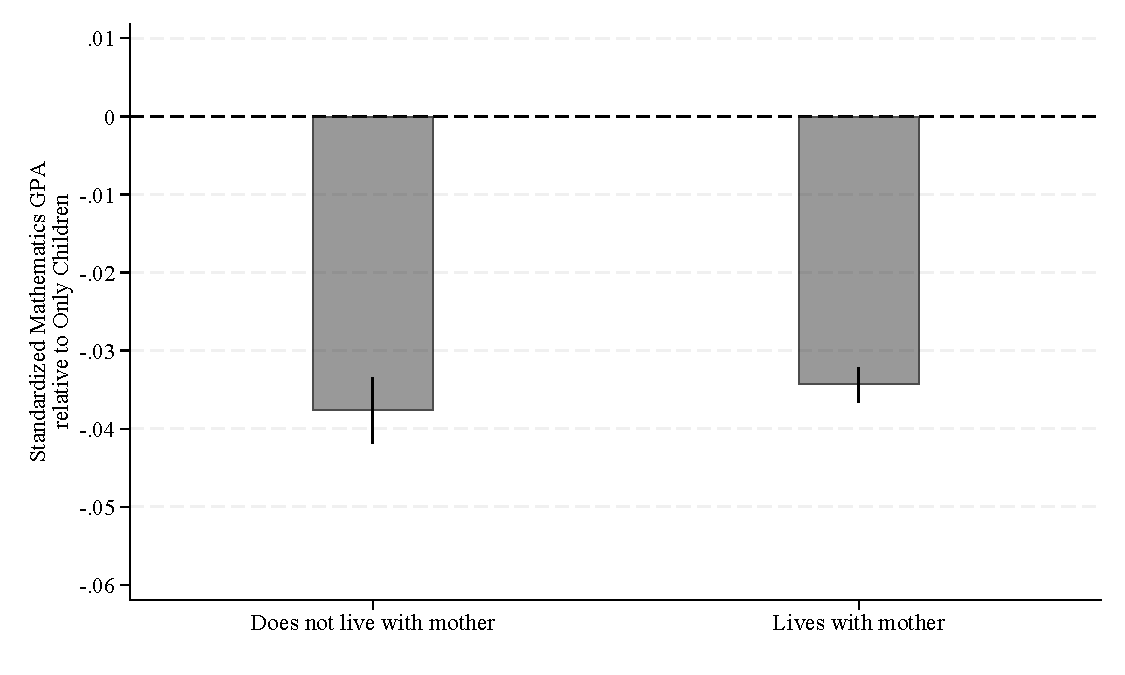
\includegraphics{./FIGURES/TWFE/twfe_gpa_lives_with_mother_20_21_Tsiblings_Soldest_4.pdf}
      }
    }

    \begin{flushleft}
        \hyperlink{frame:livesmother_siblings}{\beamergotobutton{Results by siblings}}
    \end{flushleft}    

\end{frame}

\begin{frame}
    \label{frame:livesmother_siblings}
    \frametitle{Lives with mother}
        {\resizebox{0.9\textwidth}{!}{
        %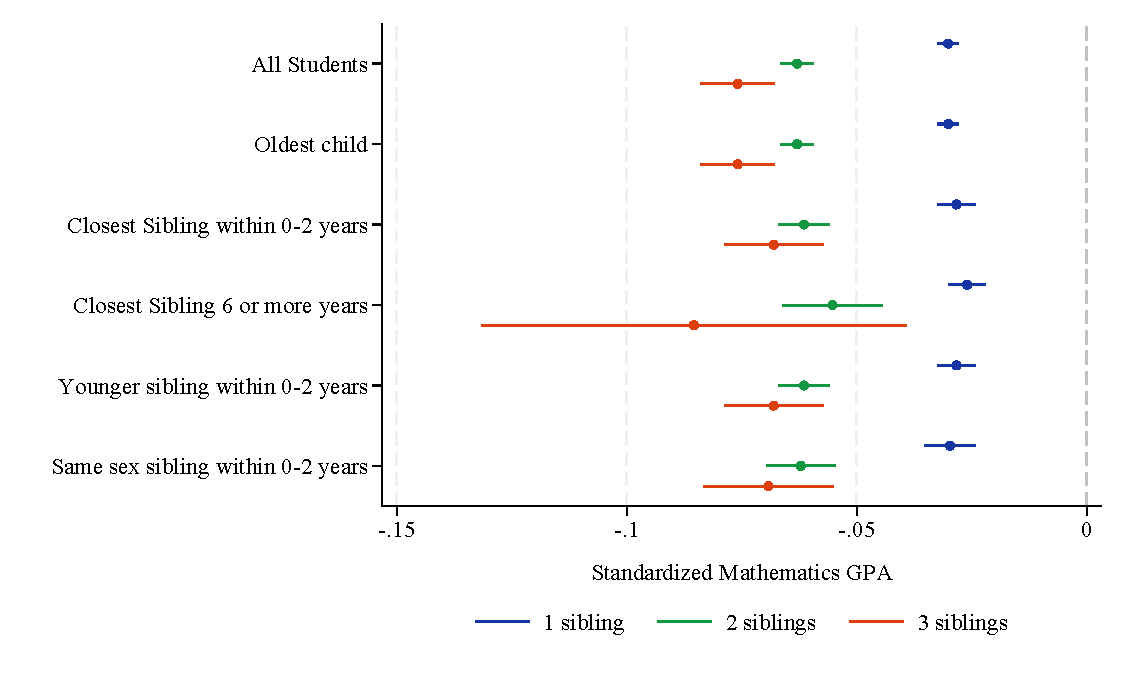
\includegraphics{./FIGURES/TWFE/covid_twfe_C_bysibs_elm_all_gpa_m_adj_Tsiblings_Soldest_4.pdf}
        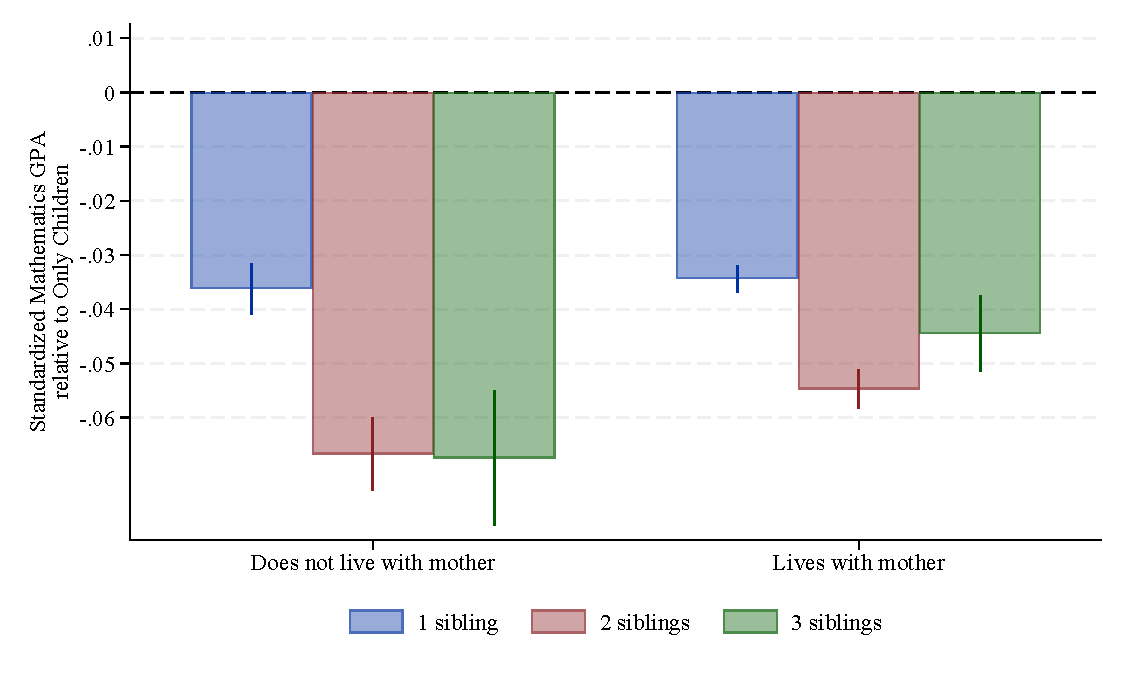
\includegraphics{./FIGURES/TWFE/twfe_gpa_lives_with_mother_bysibs_20_21_Tsiblings_Soldest_4.pdf}
      }
    }

    \begin{flushleft}
        \hyperlink{frame:livesmother}{\beamergotobutton{Go Back $\carriagereturn$}}
    \end{flushleft}        

\end{frame}
\end{comment}




\begin{frame}
    \label{frame:childcare}
    \frametitle{But does having a child at home affect parents' investment in their siblings?}
       \begin{itemize}
            \item Children who turn 6 y.o after March 31st have to wait for the next school-year to enroll in 1st grade.
            \item That creates a cutoff. \\
                Born before $\rightarrow$ children go to school \\
                Born after $\rightarrow$  they stay at home.
            \item When schools are open, this creates a negative effect for siblings both in performance and parental time invested in them.
            \item This provides some evidence of the effect of having all children stay at home during school closures.
            %\textcolor{green}{Think how to present these results...}
            %\item We use effects of delayed schooling (more childcare) outside of Covid to have a sense of how parents react to this.
            %\item Mixed results in literature (US and Denmark) although not until younger starts school.
        \end{itemize}
\end{frame}      

\begin{frame}
    \label{frame:delayedentry}
    \frametitle{Effects of delaying younger School Entry (GPA of older)}
    \makeatletter
\@ifclassloaded{beamer}{%
       \centering
       \resizebox{0.6\textwidth}{!}%
}{%
       \begin{table}[!tbp]\centering\def\sym#1{\ifmmode^{#1}\else\(^{#1}\)\fi}
       \centering
       \caption{Effects of younger sibling delaying school on older sibling standardized exams - 1 - m - a -  - 365}
       \label{tab:rd_summ_1_m_a_365}
       \resizebox{0.95\textwidth}{!}%
}
{
\makeatother
\resizebox{\textwidth}{!}{
\begin{tabular}{lccc}
\toprule
\cmidrule(lr){2-4}
& \multicolumn{3}{c}{Standardized GPA} \\
\cmidrule(lr){2-4}
& Pre-Covid & Covid & Post-Covid  \\
& 2018-2019 & 2020-2021 & 2022-2023  \\
\cmidrule(lr){2-2} \cmidrule(lr){3-3} \cmidrule(lr){4-4}
& (1) & (2) & (3)  \\
\bottomrule
&  &  &   \\
\multirow{2}{*}{\shortstack[l]{Younger sibling born after \\ school-entry cutoff}}&      -0.023***&      -0.001   &      -0.023***\\
                    &     (0.007)   &     (0.007)   &     (0.006)   \\
Local Linear        &         Yes   &         Yes   &         Yes   \\
                    &               &               &               \\
Observations        &     358,861   &     354,044   &     447,536   \\
Counterfactual mean &       0.058   &       0.020   &       0.050   \\
Bandwidth           &         365   &         365   &         365   \\
 

\bottomrule
\end{tabular}
}
\@ifclassloaded{beamer}{%
}{%
       \end{table}
}


      
    \only<2->{
    \highlightboxflex{-0.6}{-0.15}{1.2}{1.0}{draw=blue, draw opacity=0.8, dashed, fill=yellow!30, fill opacity=0.3}
    
    % Highlight box for Covid same sex coefficient  
    \highlightboxflex{1.85}{-0.15}{1.2}{1.0}{draw=blue, draw opacity=0.8, dashed, fill=yellow!30, fill opacity=0.3}
    
    \begin{tikzpicture}[overlay, remember picture]
        % Single text label at the bottom
        \node[red, above] at ([shift={(0,-2.8)}]current page.center) {\small Negative spillover of having a younger sibling stay at home};
        
        % Arrow to Pre-Covid coefficient (pointing to the left box)
        \draw[->, thick, blue, opacity=0.4] ([shift={(0,-2.2)}]current page.center) -- ([shift={(-0.6,-0.2)}]current page.center);
        
        % Arrow to Covid coefficient (pointing to the right box)
        \draw[->, thick, blue, opacity=0.4] ([shift={(0,-2.2)}]current page.center) -- ([shift={(1.85,-0.2)}]current page.center);
    \end{tikzpicture}
    }
\end{frame}

\begin{frame}
    \label{frame:delayedentryscores}
    \frametitle{Effects of delaying younger School Entry (Standardized exams and investment)}
\makeatletter
     \centering
       \resizebox{0.95\textwidth}{!}%
{
\makeatother
\begin{tabular}{lccccc}
\toprule
& \multicolumn{2}{c}{Pre-Covid}  & \multicolumn{3}{c}{Post-Covid} \\
& \multicolumn{2}{c}{2018-2019}  & \multicolumn{3}{c}{2022-2024}  \\
\cmidrule(lr){2-3} \cmidrule(lr){4-6}
& Mathematics & Reading & Mathematics & Reading & Parental Time Investment  \\
& (1) & (2) & (3) & (4) & (5) \\
\bottomrule
&  &  &  & &  \\
\multirow{2}{*}{\shortstack[l]{Younger sibling born after \\ school-entry cutoff}}&      -0.025*  &      -0.023*  &      -0.009   &      -0.012   &      -0.035***\\
                    &     (0.014)   &     (0.012)   &     (0.013)   &     (0.010)   &     (0.013)   \\
Local Linear        &         Yes   &         Yes   &         Yes   &         Yes   &         Yes   \\
                    &               &               &               &               &               \\
Observations        &      86,605   &      86,602   &     104,983   &     105,064   &     101,766   \\
Counterfactual mean &      -0.105   &      -0.083   &       0.194   &       0.288   &      -0.004   \\
Bandwidth           &         365   &         365   &         365   &         365   &         365   \\
 

\bottomrule
\end{tabular}
}

    \only<2->{

    % Highlight box for Covid same sex coefficient  
    \highlightboxflex{3.20}{-0.60}{1.2}{1.0}{draw=blue, draw opacity=0.8, dashed, fill=yellow!30, fill opacity=0.3}
    
    \begin{tikzpicture}[overlay, remember picture]
        % Single text label at the bottom
        \node[red, above] at ([shift={(0,-2.8)}]current page.center) {\small Reduces parental time investment when younger sibling stays at home};

  
        
        % Arrow to Covid coefficient (pointing to the right box)
        \draw[->, thick, blue, opacity=0.4] ([shift={(0,-2.2)}]current page.center) -- ([shift={(3.20,-0.60)}]current page.center);
    \end{tikzpicture}
    }

\end{frame}



% Show overlay 6 (Parental dilution highlighted)
\againframe<6>{mechanisms}

\begin{frame}
    \label{frame:incomeshocks_intro}
    \frametitle{Do larger families experience larger income shocks?}
    \begin{itemize}
        \item Larger learning losses in larger families could be driven by them experiencing larger income losses that may cause more disruptions in the household.
        \item When looking at an index of socio-economic status (household materials, access to services, etc.), we don't see a reduction in SES 2-4 years after the pandemic.
        \item On the contrary, there are either no effects or slight increases in the SES of children with siblings compared to only  children.
    \end{itemize}

\end{frame}


\begin{frame}
    \label{frame:incomeshocks}
    \frametitle{No evidence of negative income shocks}
     
    %\makeatletter
\@ifclassloaded{beamer}{%
       \centering
       \resizebox{0.6\textwidth}{!}%
}{%
       \begin{table}[!tbp]\centering\def\sym#1{\ifmmode^{#1}\else\(^{#1}\)\fi}
       \centering
       \caption{TWFE on Standardized Exams, Expectations and Socio-Economic Status}
       \label{tab:twfe_ece}
       \resizebox{0.8\textwidth}{!}%
}
{
\makeatother
\begin{tabular}{lccc}
\toprule
\cmidrule(lr){2-4}
& \multicolumn{3}{c}{TWFE}  \\
\cmidrule(lr){2-4}
& 1 sibling & 2 siblings & 3 siblings  \\
\cmidrule(lr){2-2} \cmidrule(lr){3-3} \cmidrule(lr){4-4}
& (1) & (2) & (3)\\
\bottomrule
&  &  &  \\
&  &  &   \\
\multicolumn{4}{l}{\textit{Panel A: 2nd grade students}} \\
\hspace{3mm}Mathematics&      -0.028** &      -0.090***&      -0.093   \\
                    &     (0.011)   &     (0.023)   &     (0.081)   \\
 
%&  &  &   \\
\hspace{3mm}Reading &      -0.028** &      -0.068***&      -0.140*  \\
                    &     (0.011)   &     (0.022)   &     (0.078)   \\
 
%&  &  &   \\
\hspace{3mm}Max Expectation: Finish school&       0.008***&      -0.002   &      -0.026   \\
                    &     (0.003)   &     (0.006)   &     (0.022)   \\
 
%&  &  &   \\
\hspace{3mm}Max Expectation: 4-year college&      -0.011** &       0.004   &      -0.010   \\
                    &     (0.004)   &     (0.009)   &     (0.034)   \\
 
%&  &  &   \\
\hspace{3mm}SES     &       0.018** &       0.022   &       0.058   \\
                    &     (0.009)   &     (0.019)   &     (0.069)   \\
 
&  &  &   \\
\multicolumn{4}{l}{\textit{Panel B: 4th grade students}} \\
\hspace{3mm}Mathematics&      -0.022***&      -0.103***&      -0.172***\\
                    &     (0.004)   &     (0.008)   &     (0.022)   \\
 
%&  &  &   \\
\hspace{3mm}Reading &      -0.027***&      -0.103***&      -0.139***\\
                    &     (0.004)   &     (0.008)   &     (0.022)   \\
 
%&  &  &   \\
\hspace{3mm}Max Expectation: Finish school&       0.006***&       0.004   &       0.005   \\
                    &     (0.001)   &     (0.003)   &     (0.008)   \\
 
%&  &  &   \\
\hspace{3mm}Max Expectation: 4-year college&      -0.012***&      -0.020***&      -0.032***\\
                    &     (0.002)   &     (0.004)   &     (0.010)   \\
 
%&  &  &   \\
\hspace{3mm}SES     &       0.017***&      -0.005   &       0.004   \\
                    &     (0.003)   &     (0.006)   &     (0.019)   \\
 
&  &  &   \\
\multicolumn{4}{l}{\textit{Panel C: 8th grade students}} \\
\hspace{3mm}Mathematics&      -0.014** &      -0.036***&      -0.029   \\
                    &     (0.007)   &     (0.010)   &     (0.018)   \\
 
%&  &  &   \\
\hspace{3mm}Reading &       0.005   &      -0.009   &      -0.023   \\
                    &     (0.007)   &     (0.009)   &     (0.017)   \\
 
%&  &  &   \\
\hspace{3mm}Max Expectation: Finish school&      -0.011   &      -0.001   &       0.051***\\
                    &     (0.010)   &     (0.013)   &     (0.019)   \\
 
%&  &  &   \\
\hspace{3mm}Max Expectation: 4-year college&      -0.007   &      -0.003   &      -0.054** \\
                    &     (0.014)   &     (0.017)   &     (0.026)   \\
 
%&  &  &   \\
\hspace{3mm}SES     &       0.017***&       0.026***&       0.038***\\
                    &     (0.005)   &     (0.008)   &     (0.014)   \\
 

\bottomrule
\end{tabular}
}
\@ifclassloaded{beamer}{%
}{%
       \end{table}
}


     {\resizebox{0.9\textwidth}{!}{
        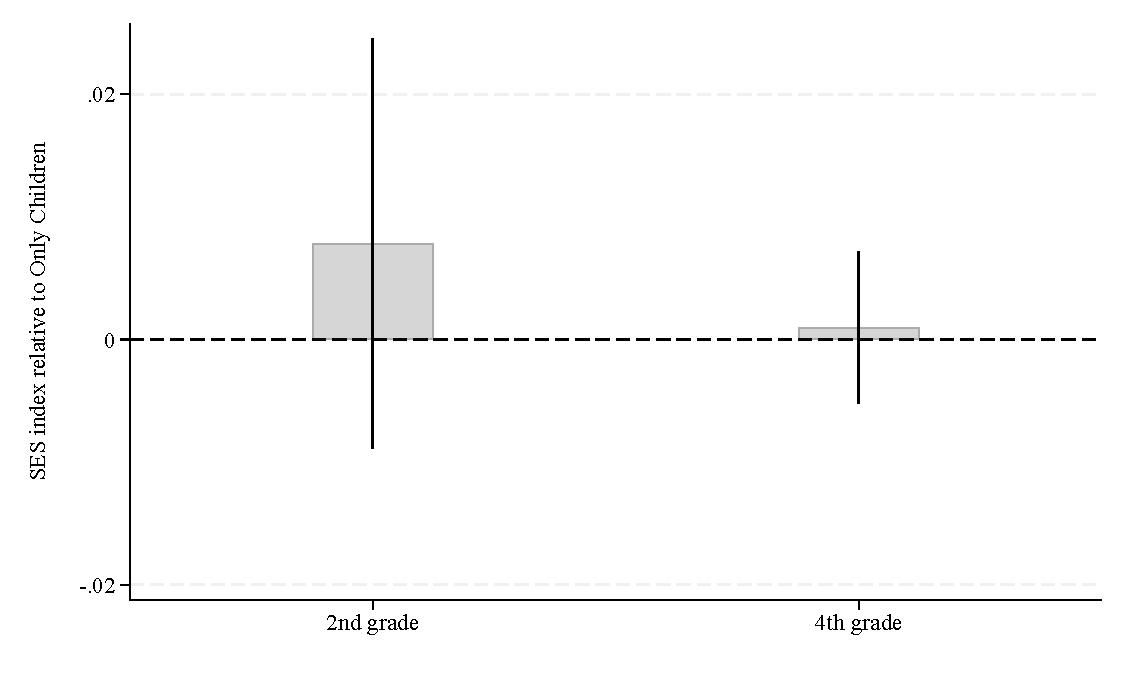
\includegraphics{./FIGURES/TWFE/twfe_ses_2_4_Tsiblings_Soldest_4.pdf}
      }
    }

    \begin{flushleft}
        \hyperlink{frame:incomeshocks_siblings}{\beamergotobutton{Results by siblings}}
    \end{flushleft}  

   
\end{frame}




\begin{frame}
    \label{frame:iv_intro}
    \frametitle{Remaining endogeneity: Using Same Sex and Twin IV}
    \begin{itemize}
        \item To address any further remaining endogeneity concerns such as time-varying unobserved shocks we use an IV approach.
        \item Having same sex children (Boy-boy or girl-girl) makes families more likely to have a third child. Twin births is also used as a potential exogenous variation in family size.
        \item this captures family size effects in families with at least 2 children.
    \end{itemize}    
   
\end{frame}

\begin{frame}[t]
    \label{frame:iv_results}
    \frametitle{Same sex IV shows a reduction in family size effect during closures}
    \begin{table}[h]
\centering
\caption{Effect of Family Size on GPA}
\label{tab:twfe_twins}
\resizebox{0.95\textwidth}{!}{%
\begin{tabular}{lHccccHcccc}
\hline
& \multicolumn{5}{c}{Pre-Covid} & \multicolumn{5}{c}{Covid (2020-2021)} \\
\cmidrule(lr){2-6} \cmidrule(lr){7-11}
& OLS & OLS & First & Second & N & OLS & OLS & First & Second & N \\
& (no controls) & (controls) & Stage & Stage & & (no controls) & (controls) & Stage & Stage & \\
\hline
& & & & & & & & & & \\
Instrument: first two children same sex & & & 0.050* & & 3,300,349 & & & 0.047* & & 2,809,126 \\
\quad (Sample: first and second children in families & & & (0.001) & & & & & (0.001) & & \\
\quad with two or more births) & & & & & & & & & & \\
Number of children in family & $-0.081$* & $-0.070$* & & 0.063* & & $-0.119$* & $-0.101$* & & $-0.031$ & \\
& (0.001) & (0.001) & & (0.022) & & (0.001) & (0.001) & & (0.025) & \\
Instrument: twin at second birth & & & 0.813* & & 1,589,159 & & & 0.855* & & 1,240,864 \\
\quad (Sample: First child in families with two or more & & & (0.006) & & & & & (0.006) & & \\
\quad births) & & & & & & & & & & \\
Number of children in family & $-0.090$* & $-0.056$* & & 0.012 & & $-0.125$* & $-0.085$* & & 0.009 & \\
& (0.001) & (0.001) & & (0.012) & & (0.002) & (0.002) & & (0.013) & \\
& & & & & & & & & & \\
%Instrument: twin at third birth & & & 0.819* & & 1,195,717 & & & 0.866* & & 841,770 \\
%\quad (Sample: first and second children in families & & & (0.006) & & & & & (0.006) & & \\
%\quad with three or more births) & & & & & & & & & & \\
%Number of children in family & $-0.104$* & $-0.090$* & & $-0.020$ & & $-0.118$* & $-0.101$* & & $-0.019$ & \\
%& (0.002) & (0.002) & & (0.013) & & (0.002) & (0.002) & & (0.014) & \\
%& & & & & & & & & & \\
\hline
\end{tabular}%
}
\end{table}
   
    \only<2->{
    \highlightboxflex{0.3}{-0.25}{0.8}{0.7}{draw=blue, draw opacity=0.8, dashed, fill=yellow!30, fill opacity=0.3}
    
    % Highlight box for Covid same sex coefficient  
    \highlightboxflex{3.55}{-0.25}{0.8}{0.7}{draw=blue, draw opacity=0.8, dashed, fill=yellow!30, fill opacity=0.3}
    
    \begin{tikzpicture}[overlay, remember picture]
        % Single text label at the bottom
        \node[red, above] at ([shift={(0,-2.8)}]current page.center) {\small Reduction in family size effect! \\ $\Delta$ = -.094*};
        
        % Arrow to Pre-Covid coefficient (pointing to the left box)
        \draw[->, thick, blue, opacity=0.4] ([shift={(0,-1.8)}]current page.center) -- ([shift={(0.3,-0.25)}]current page.center);
        
        % Arrow to Covid coefficient (pointing to the right box)
        \draw[->, thick, blue, opacity=0.4] ([shift={(0,-1.8)}]current page.center) -- ([shift={(3.55,-0.25)}]current page.center);
    \end{tikzpicture}
    }
\end{frame}

\begin{frame}
    \label{frame:iv_conclusion}
    \frametitle{Effect of family size on GPA: Using Same Sex and Twin IV}
 \begin{itemize}
        \item We see a negative reduction in family size effects on performance using same sex IV.
        \item Twin IV might not be well suited for this context. Parents may be more able to teach, study and help siblings that share coursework.
        %\item One reason why we don't find results could be that to some this captures more the effect of monetary cost but in terms of time, twins might not be twice as costly than two separate children
        \item We are estimating here the differential effect from \#2 to \#3,\#4, etc. Not from single children to children with siblings.
    \end{itemize}
\end{frame}

% ========================================
% BEYOND PERFORMANCE
% ========================================
\section{Beyond performance}

    \begin{frame}
            \label{frame:expectations}
            \frametitle{Reduction in educational expectations}
      {\resizebox{0.9\textwidth}{!}{
        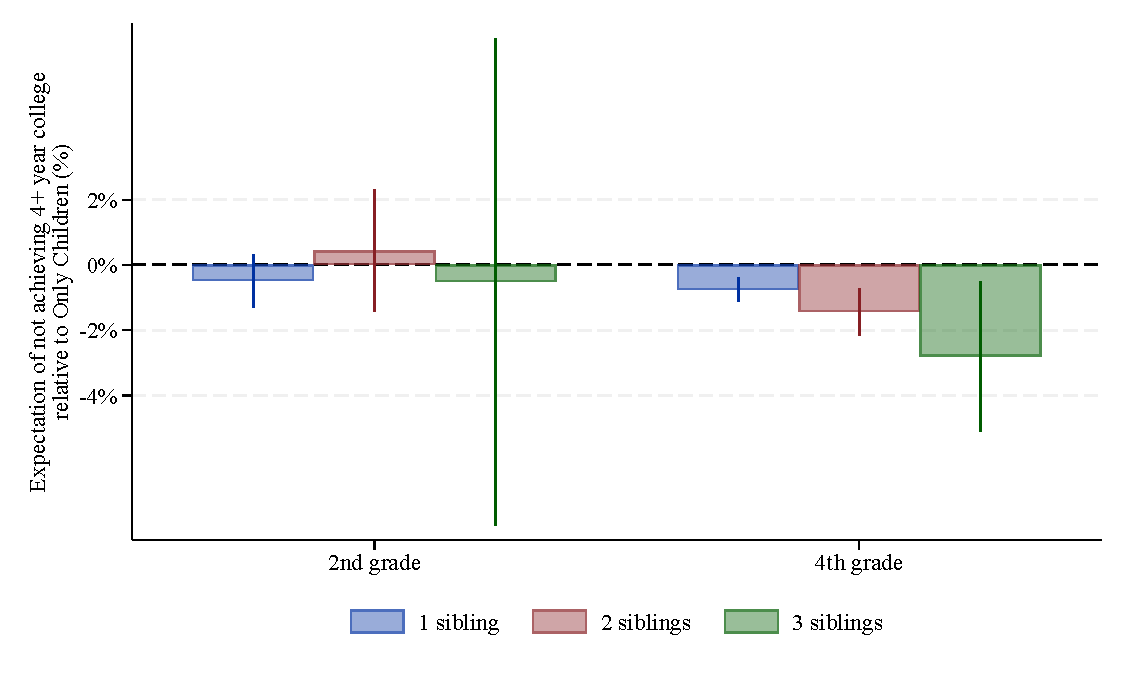
\includegraphics{./FIGURES/TWFE/twfe_expectation_bysibs_2_4_Tsiblings_Soldest_4.pdf}
      }
    }   %\input{./TABLES/MANUAL/twfe_ece_expectations.tex}
    \end{frame}

 \begin{frame}
            \label{frame:dropout_risk_intro}
            \frametitle{Risk of dropout}
       \begin{itemize}
           \item During school closures, students are automatically promoted to the next grade.
           \item If no evidence was provided from students, their grade would be left blank.
           \item Similar to \cite{lichand_impacts_2021}, I estimate risk of dropout by looking at the percentage of students without a grade.
           \item I see that dropout risk increases during school closures for children with siblings.
       \end{itemize}
    \end{frame} 


    \begin{frame}
            \label{frame:dropout_risk}
            \frametitle{Increased likelihood of dropout with number of siblings}
        {\resizebox{0.9\textwidth}{!}{
        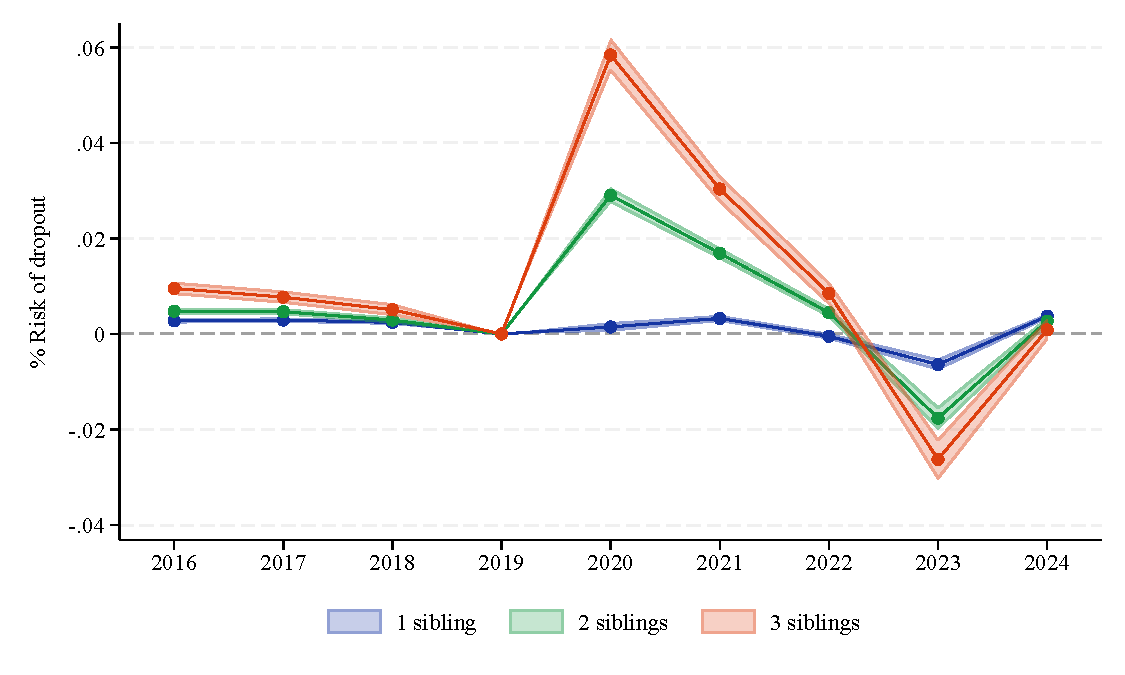
\includegraphics{./FIGURES/Event Study/covid_event_bysibs_elm_all_dropout_risk_Tsiblings_Soldest_4.pdf}
      }
    }   %\input{./TABLES/MANUAL/twfe_ece_expectations.tex}
   
    \end{frame}   

    \begin{frame}
            \label{frame:ece_gender}
            \frametitle{Heterogeneity by gender}
        {\resizebox{0.9\textwidth}{!}{
        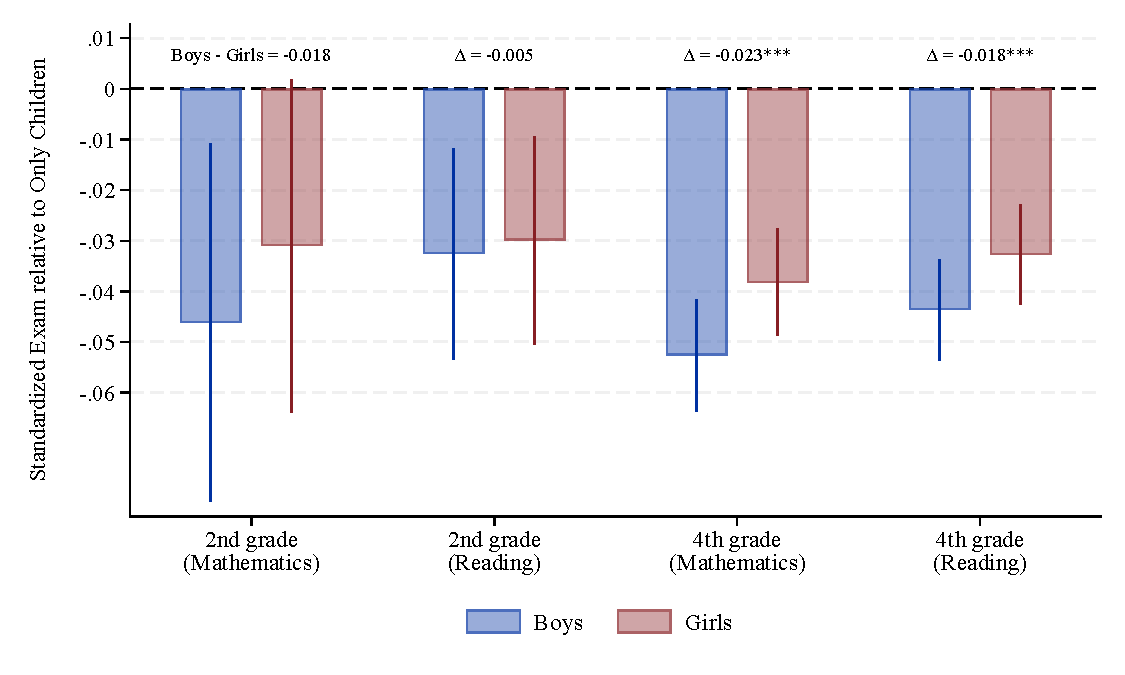
\includegraphics{./FIGURES/TWFE/ece_2_4_gender_Tsiblings_Soldest.pdf}
      }
    }   %\input{./TABLES/MANUAL/twfe_ece_expectations.tex}
   
    \end{frame} 
    

\begin{comment}
    \begin{frame}
            \label{frame:college_app}
            \frametitle{College Applications}
   \textcolor{green}{Pending}
    %\input{./TABLES/MANUAL/twfe_ece_expectations.tex}
    \end{frame}      
\end{comment}
% ========================================
% EXTERNAL VALIDITY
% ========================================



% ========================================
% CONCLUSIONS
% ========================================
\section{Conclusions}

\begin{frame}
    \label{frame:conclusions}
    \frametitle{Conclusions}
    \begin{itemize}
        \item Households are not able to adequately compensate for school closures. With more children, parents have more difficulty investing sufficient time in each of them. 
        \item Children with siblings engage less, obtain worse grades and have lower performance in standardized tests years after schools reopened.
        \item Parental time investment, rather than sibling competition for resources is the main mechanism behind this effects.
        \item Low SES families, which have the lowest investment in their children, exhibit lower tradeoffs.
    \end{itemize}
\end{frame}


\begin{frame}
    \hypersetup{citecolor=blue}
  \centering
  \vspace{2cm}
  {\Huge \textbf{Thank you!}} \\[1cm]
  
  {\Large Questions or comments?} \\[0.5cm]
  
  \rule{0.4\linewidth}{0.4pt} \\[0.5cm]
  
  \begin{flushleft}
    \textbf{Francisco Pardo} \\
    University of Texas at Austin \\
    fpardo@utexas.edu \\
    %\href{mailto:fpardo@utexas.edu}{fpardo@utexas.edu} \\
    \href{https://francisco-pardo-pajuelo.github.io/}{Website}
  \end{flushleft}

\end{frame}





% ========================================
% EXAMPLE SLIDES
% ========================================
\section{Resources}





\begin{frame}[allowframebreaks]
    \frametitle{References}
    \small
    \tiny\bibliography{references}  % <- Call your .bib file here (no .bib extension)
\end{frame}


% ========================================
% NAVIGATION SLIDE - COMPACT VERSION
% ========================================
\begin{frame}
    \label{frame:navigation}
    \frametitle{Presentation Navigation}
    
    \small % Reduce overall font size
    
    \begin{columns}[T]
        \begin{column}{0.45\textwidth}
            \centering
            \textbf{Introduction \& Setup}
            \vspace{0.1cm}
            
            \hyperlink{frame:motivation}{\beamergotobutton{Motivation}}\\[2pt]
            %\hyperlink{frame:thispaper}{\beamergotobutton{This Paper}}\\[2pt]
            \hyperlink{frame:contribution}{\beamergotobutton{Literature}}\\[2pt]
            \hyperlink{frame:background}{\beamergotobutton{Background}}\\[2pt]
            \hyperlink{frame:data}{\beamergotobutton{Data}}\\[2pt]
            \hyperlink{frame:ece_trends}{\beamergotobutton{Descriptive}}
            
            \vspace{0.2cm}
            \textbf{Mechanisms}
            \vspace{0.1cm}
            
            \hyperlink{frame:mechanisms}{\beamergotobutton{Potential Mechanisms}}\\[2pt]
            \hyperlink{frame:birthorder}{\beamergotobutton{Birth Order}}\\[2pt]
            \hyperlink{frame:resources_intro}{\beamergotobutton{Resource Competition}} \\[2pt]
            \hyperlink{frame:siblingdisruption_intro}{\beamergotobutton{Sibling Disruption}} \\[2pt]
            \hyperlink{frame:parentaldilution_intro}{\beamergotobutton{Parental Resources}} \\[2pt]
            \hyperlink{frame:parental_investments_vs_ses}{\beamergotobutton{Parental Investment vs SES}} \\[2pt]
            \hyperlink{frame:byses}{\beamergotobutton{Analysis by SES}}\\[2pt]
            \hyperlink{frame:childcare}{\beamergotobutton{Childcare Effects}}\\[2pt]
            %\hyperlink{frame:delayedentry}{\beamergotobutton{Delayed Entry}}\\[2pt]
            %\hyperlink{frame:delayedentryscores}{\beamergotobutton{Delayed Entry Scores}} \\[2pt]
            \hyperlink{frame:incomeshocks}{\beamergotobutton{Income Shocks}}              
        \end{column}
        
        \begin{column}{0.45\textwidth}
            \centering
            \textbf{Methodology \& Results}
            \vspace{0.1cm}
            
            \hyperlink{frame:research}{\beamergotobutton{Research Design}}\\[2pt]
            \hyperlink{frame:empirical}{\beamergotobutton{Empirical Strategy}}\\[2pt]
            \hyperlink{frame:eventstudy}{\beamergotobutton{Event Study}}\\[2pt]
            \hyperlink{frame:twfe_gpa_2_4_6_8}{\beamergotobutton{TWFE Results}}\\[2pt]
            \hyperlink{frame:twfe_gpa_2_4_8}{\beamergotobutton{Standardized Exams}}
            \hyperlink{frame:twfe_gpa_controls}{\beamergotobutton{TWFE with controls}}

            
            
            \vspace{0.2cm}
            \textbf{Additional Analysis}
            \vspace{0.1cm}
        
            \hyperlink{frame:otherstrategies}{\beamergotobutton{Other Strategies}}\\[2pt]
            \hyperlink{frame:iv_intro}{\beamergotobutton{Twin IV}} \\[2pt]
            \hyperlink{frame:expectations}{\beamergotobutton{Expectations}} \\[2pt]
            \hyperlink{frame:dropout_risk}{\beamergotobutton{Risk of Dropout}} \\[2pt]
            \hyperlink{frame:ece_gender}{\beamergotobutton{Gender Heterogeneity}}

            \vspace{0.2cm}
            \textbf{Conclusions}
            \vspace{0.1cm}
            
            %\hyperlink{frame:pisadata}{\beamergotobutton{PISA Data}} \\[2pt]
            %\hyperlink{frame:pisagaps}{\beamergotobutton{Learning Gaps}} \\[2pt]
            %\hyperlink{frame:pisaclosure}{\beamergotobutton{School Closure}} \\[2pt]
            \hyperlink{frame:conclusions}{\beamergotobutton{Conclusions}}
            
        \end{column}
    \end{columns}
    

\end{frame}

\begin{comment}
\begin{frame}
    \label{frame:highlightfigure}
    \frametitle{Highlighting Parts of slide}
    \highlightboxflex{-3.5}{0.5}{1.5}{1.5}{draw=blue, draw opacity=0.8, dashed, fill=yellow!30, fill opacity=0.3}
    \begin{tikzpicture}[overlay, remember picture]
        \node[red, above] at ([shift={(-2.75,2.2)}]current page.center) {\small Key finding!};
        \draw[->, thick, blue, opacity=0.8] ([shift={(-2.5,-2.5)}]current page.center) -- ([shift={(-3.1,0.5)}]current page.center);
%blue!50!black
    \end{tikzpicture}
\end{frame}
\end{comment}


%%%%%%%%%%%%%%%%%%%%%%%%%%%%%%%%%%%%%%%%%%%%%%%%%%%%%
\section{GPA Trends by grade}
%%%%%%%%%%%%%%%%%%%%%%%%%%%%%%%%%%%%%%%%%%%%%%%%%%%%%




\begin{frame}
    \label{frame:gpa_trends_grades_elm}
    \frametitle{Trends in data}
               \includegraphics[width=\textwidth]{./FIGURES/Descriptive/raw_grades_elm_std_gpa_m_adj_Tsiblings_Sall_Size2_4.pdf}    
    \begin{flushleft}
        \hyperlink{frame:gpa_trends}{\beamergotobutton{Go Back $\carriagereturn$}}
    \end{flushleft}   
    
    
\end{frame}

\begin{frame}
    \label{frame:gpa_trends_grades_sec}
    \frametitle{Trends in data}
               \includegraphics[width=\textwidth]{./FIGURES/Descriptive/raw_grades_sec_std_gpa_m_adj_Tsiblings_Sall_Size2_4.pdf}    
          \hyperlink{frame:gpa_trends}{\beamergotobutton{Go Back $\carriagereturn$}}
  
\end{frame}




\begin{comment}
\begin{frame}
    \label{frame:twfe}
    \frametitle{TWFE results}
        {\resizebox{0.9\textwidth}{!}{
       %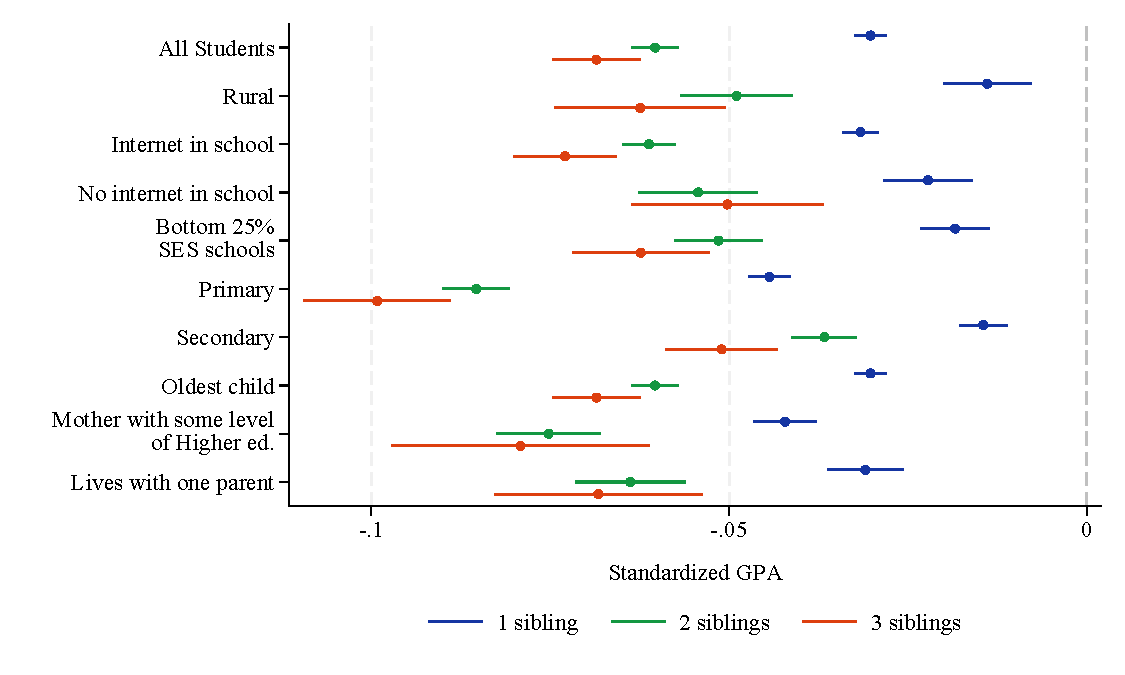
\includegraphics{./FIGURES/TWFE/covid_twfe_summ_bysibs_all_20-21_gpa_m_adj_Tsiblings_Soldest_4.pdf}
       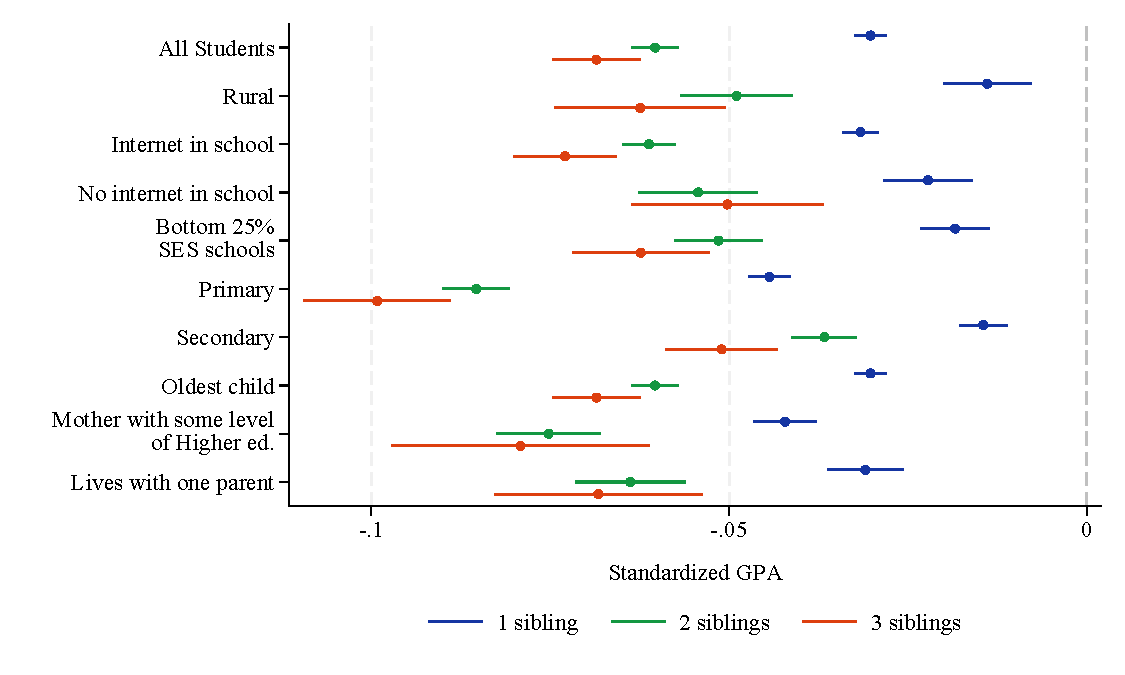
\includegraphics{./FIGURES/TWFE/covid_twfe_summ_bysibs_all_20-21_gpa_m_adj_Tsiblings_Soldest_4.pdf}
      }
    }
\end{frame}

\begin{frame}
\label{frame:twfeexams}
\frametitle{TWFE - Standardized Exams}
       \centering
       \resizebox{0.7\textwidth}{!}%
{
\makeatother
\begin{tabular}{lcccc}
\toprule
\cmidrule(lr){2-5}
& \multicolumn{4}{c}{TWFE} \\
\cmidrule(lr){2-5}
& 1-3 siblings & 1 sibling & 2 siblings & 3 siblings  \\
\cmidrule(lr){2-2} \cmidrule(lr){3-3} \cmidrule(lr){4-4} \cmidrule(lr){5-5}
& (1) & (2) & (3) & (4) \\
\bottomrule
&  &  & &  \\
&  &  & &  \\
\multicolumn{5}{l}{Panel A: GPA } \\
Mathematics         &      -0.099***&      -0.011   &      -0.036***&      -0.059***\\
                    &     (0.009)   &     (0.009)   &     (0.011)   &     (0.015)   \\
                    &               &               &               &               \\ 
&  &  & &  \\
Reading             &      -0.099***&      -0.010   &      -0.031***&      -0.034** \\
                    &     (0.009)   &     (0.009)   &     (0.010)   &     (0.015)   \\
                    &               &               &               &               \\
Observations        &     326,669   &     280,846   &     225,840   &     180,218   \\
 
&  &  & &  \\
\multicolumn{5}{l}{Panel B: Standardized Exams } \\
Mathematics         &      -0.034***&      -0.017** &      -0.044***&      -0.071***\\
                    &     (0.006)   &     (0.007)   &     (0.008)   &     (0.011)   \\
                    &               &               &               &               \\ 
&  &  & &  \\
Reading             &      -0.013** &       0.002   &      -0.022***&      -0.046***\\
                    &     (0.006)   &     (0.006)   &     (0.008)   &     (0.011)   \\
                    &               &               &               &               \\
Observations        &     409,690   &     282,769   &     227,486   &     181,466   \\
 

\bottomrule
\end{tabular}
}

\end{frame}


\begin{frame}
    \label{frame:ses}
    \frametitle{Scarce material resources: Socio Economic Status}
       \centering
       \resizebox{0.7\textwidth}{!}{
\makeatother
\begin{tabular}{lcccc}
\toprule
\cmidrule(lr){2-5}
& \multicolumn{4}{c}{TWFE} \\
\cmidrule(lr){2-5}
& 1-3 siblings & 1 sibling & 2 siblings & 3 siblings  \\
\cmidrule(lr){2-2} \cmidrule(lr){3-3} \cmidrule(lr){4-4} \cmidrule(lr){5-5}
& (1) & (2) & (3) & (4) \\
\bottomrule
&  &  & &  \\
&  &  & &  \\

\multicolumn{5}{l}{Panel B: Low SES Households (Q1)} \\
Mathematics         &      -0.028***&      -0.009   &      -0.036***&      -0.061***\\
                    &     (0.005)   &     (0.006)   &     (0.006)   &     (0.008)   \\
 
&  &  & &  \\
Reading             &      -0.022***&      -0.010   &      -0.029***&      -0.044***\\
                    &     (0.005)   &     (0.006)   &     (0.007)   &     (0.008)   \\
                    &               &               &               &               \\
Observations        &     643,621   &     398,084   &     358,488   &     290,244   \\
 
&  &  & &  \\
\multicolumn{5}{l}{Panel C: High SES Households (Q4)} \\
Mathematics         &      -0.035***&      -0.029***&      -0.051***&      -0.072***\\
                    &     (0.006)   &     (0.007)   &     (0.009)   &     (0.019)   \\
 
&  &  & &  \\
Reading             &      -0.039***&      -0.032***&      -0.068***&      -0.010   \\
                    &     (0.006)   &     (0.007)   &     (0.010)   &     (0.019)   \\
                    &               &               &               &               \\
Observations        &     385,616   &     318,633   &     230,174   &     186,296   \\
 

\bottomrule
\end{tabular}
}

\end{frame}



\begin{transitionframe}
    \label{frame:parentaldilution_summary}
    \frametitle{Parental dilution}
        {\resizebox{0.9\textwidth}{!}{
        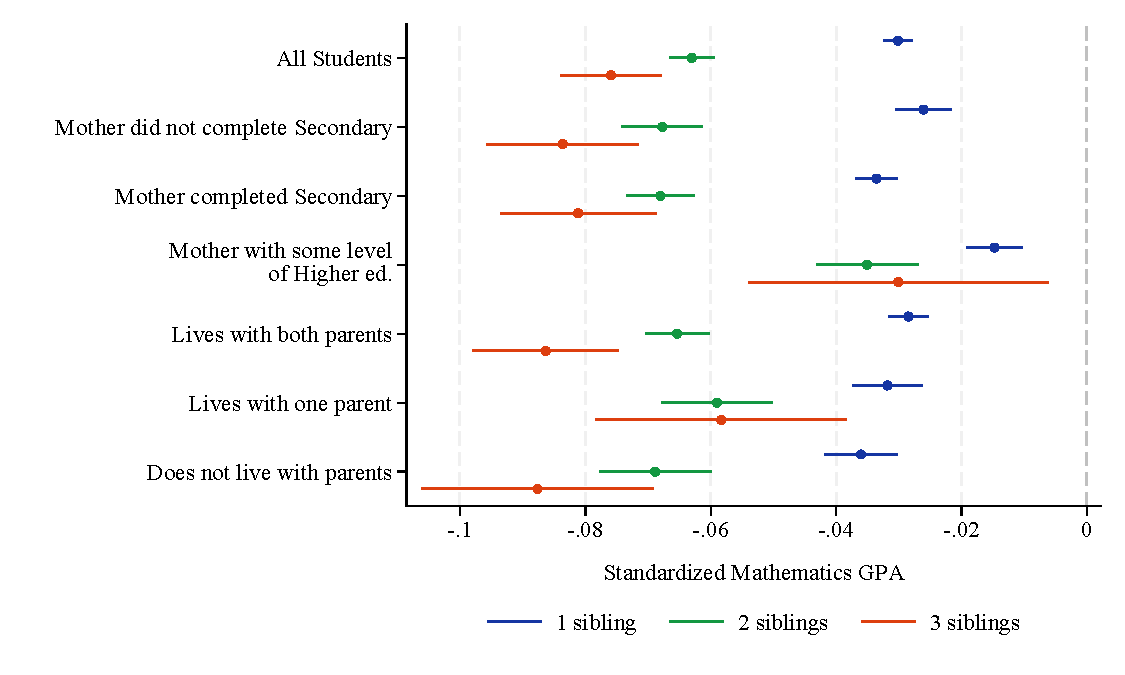
\includegraphics{./FIGURES/TWFE/covid_twfe_D_bysibs_elm_all_gpa_m_adj_Tsiblings_Soldest_4.pdf}%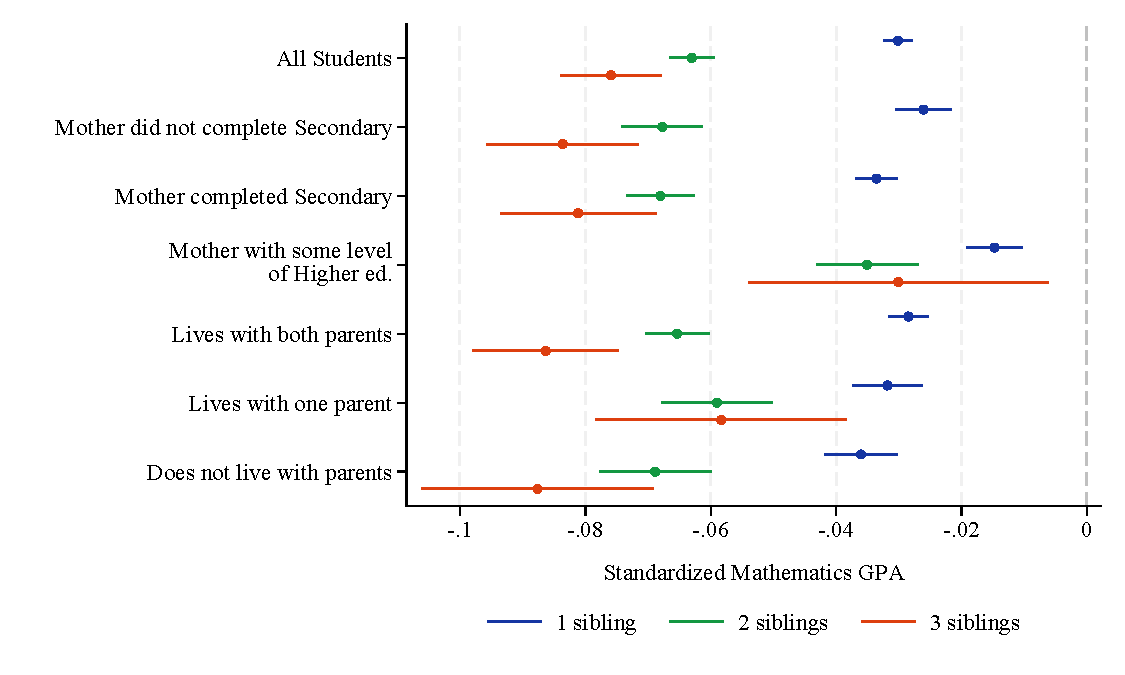
\includegraphics{./FIGURES/TWFE/covid_twfe_D_bysibs_elm_all_gpa_m_adj_Tsiblings_Soldest_4.pdf}
      }
    }

\end{transitionframe}


\begin{transitionframe}
    \label{frame:pcinternet_table}
    \frametitle{Scarce material resources: PC and Internet}
       \centering
       \resizebox{0.7\textwidth}{!}{
\makeatother
\begin{tabular}{lcccc}
\toprule
\cmidrule(lr){2-5}
& \multicolumn{4}{c}{TWFE} \\
\cmidrule(lr){2-5}
& 1-3 siblings & 1 sibling & 2 siblings & 3 siblings  \\
\cmidrule(lr){2-2} \cmidrule(lr){3-3} \cmidrule(lr){4-4} \cmidrule(lr){5-5}
& (1) & (2) & (3) & (4) \\
\bottomrule
&  &  & &  \\
\multicolumn{5}{l}{Panel D: Households with no PC or Internet} \\
Mathematics         &      -0.037***&      -0.024***&      -0.067***&      -0.089***\\
                    &     (0.005)   &     (0.005)   &     (0.006)   &     (0.010)   \\
 
&  &  & &  \\
Reading             &      -0.036***&      -0.025***&      -0.063***&      -0.083***\\
                    &     (0.005)   &     (0.005)   &     (0.006)   &     (0.010)   \\
                    &               &               &               &               \\
Observations        &     766,875   &     566,628   &     447,252   &     356,075   \\
 
&  &  & &  \\
\multicolumn{5}{l}{Panel E: Households with both PC and Internet} \\
Mathematics         &      -0.043***&      -0.024***&      -0.051***&      -0.080***\\
                    &     (0.005)   &     (0.005)   &     (0.006)   &     (0.008)   \\
 
&  &  & &  \\
Reading             &      -0.035***&      -0.018***&      -0.049***&      -0.054***\\
                    &     (0.005)   &     (0.005)   &     (0.006)   &     (0.008)   \\
                    &               &               &               &               \\
Observations        &     793,797   &     552,557   &     452,886   &     360,214   \\
 

\bottomrule
\end{tabular}
}

\end{transitionframe}
\end{comment}
%%%%%%%%%%%%%%%%%%%%%%%%%%%%%%%%%%%%%%%%%%%%%%%%%%%%%
\section{External Validity}
%%%%%%%%%%%%%%%%%%%%%%%%%%%%%%%%%%%%%%%%%%%%%%%%%%%%%

    \begin{frame}
            \label{frame:pisadata}
            \frametitle{Is this only about Peru?}
        \begin{itemize}
            \item International examination to 15 year olds
            \item 81 countries (37 OECD and 44 non-OECD).
            \item In 2009, 2012 and 2022, I am able to identify only-child and sibling sample.
            \item In most countries, children with siblings also exhibit larger learning losses
            \item Longer school closures where associated with larger gaps.
        \end{itemize}
    \end{frame}

\begin{frame}
    \label{frame:pisagaps}
    \frametitle{Learning gaps in Mathematics by year}
    
    \begin{figure}
        \centering
        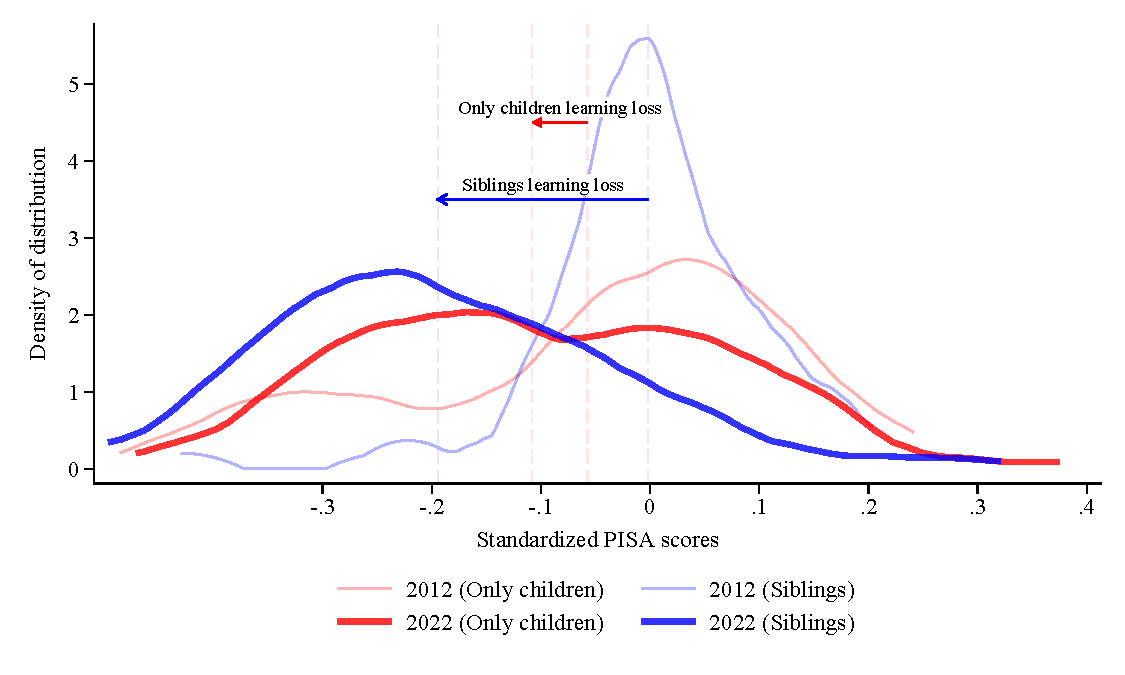
\includegraphics[width=0.9\textwidth]{./FIGURES/Descriptive/PISA_distribution_2012_2022_PV4MATH.pdf}
        \caption{Learning gaps in Mathematics by year}
        \label{fig:1a}
    \end{figure}
    
\end{frame}

\begin{frame}
    \label{frame:pisaclosure}
    \frametitle{Change in learning gaps by duration of school closure}
    
    \begin{figure}
        \centering
        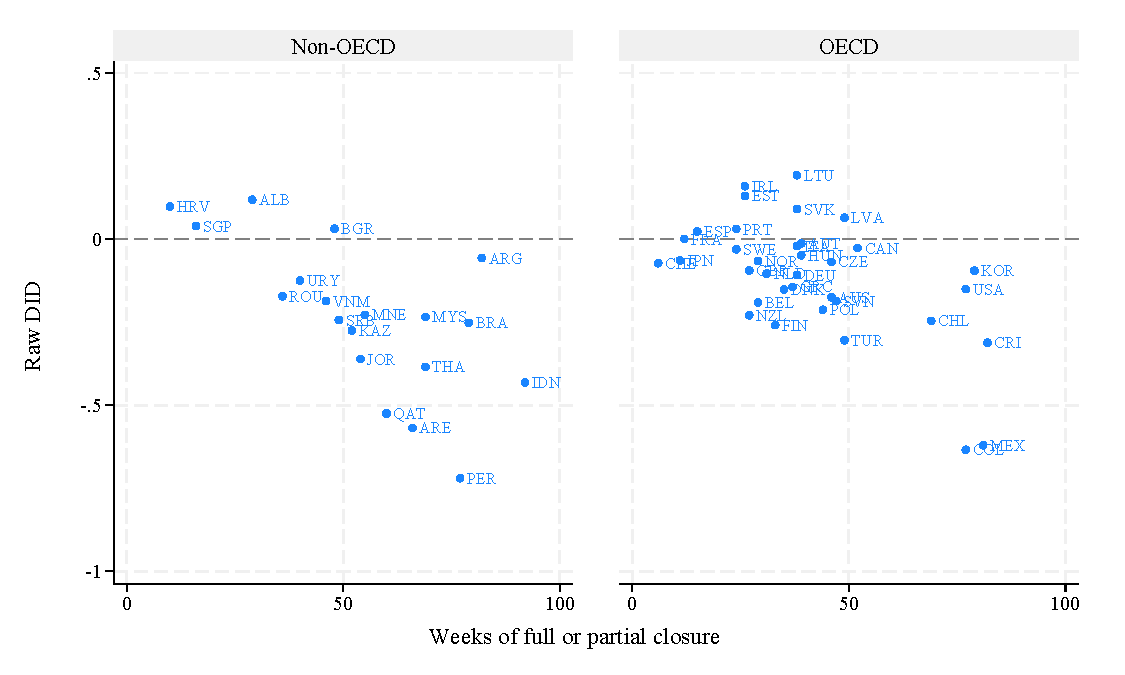
\includegraphics[width=0.9\textwidth]{./FIGURES/Descriptive/PISA_raw_DID_PV4MATH_not_fully_open.pdf}
        \caption{Similar pattern in rest of the world}
        \label{fig:1b}
    \end{figure}
    
    
\end{frame}


\begin{frame}[T]
    \label{frame:india}
    \frametitle{India exhibits similar heterogeneity}
    
      %
\begingroup
\setlength{\tabcolsep}{2pt} % Default value: 6pt
\begin{table}[H]
\centering
\footnotesize
%\begin{threeparttable}
\centering
\caption{Learning loss between August 2019 and December 2021}
\label{tab:india}
\resizebox{1\linewidth}{!}{
\begin{tabular}{lcccccccccccc}
\toprule
& (1) & (2) & (3) & (4) & (5) & (6) & (7) & (8) & (9) & (10) & (11) & (12) \\
\midrule
\multicolumn{8}{l}{\textbf{Panel B: Learning loss in regression form}}\\
&	\multicolumn{6}{c}{Math score (in SD)}&	\multicolumn{6}{c}{Tamil score (in SD)} \\
 \cmidrule(lr){2-7} \cmidrule(lr){8-13}
Wave 1 (Dec 2021)   &        -.73\sym{***}&        -.74\sym{***}&        -.76\sym{***}&        -.75\sym{***}&        -.68\sym{***}&        -.71\sym{***}&        -.35\sym{***}&        -.35\sym{***}&        -.37\sym{***}&        -.38\sym{***}&        -.32\sym{***}&        -.34\sym{***}\\
                    &      (.031)         &      (.038)         &      (.042)         &      (.049)         &      (.037)         &      (.046)         &       (.02)         &      (.023)         &      (.027)         &      (.029)         &      (.024)         &      (.031)         \\
Male $\times$ Dec 21&                     &        .023         &                     &                     &                     &                     &                     &      -.0074         &                     &                     &                     &                     \\
                    &                     &      (.041)         &                     &                     &                     &                     &                     &      (.022)         &                     &                     &                     &                     \\
Mother Edu: Gr. 9-11 $\times$ Dec 21&                     &                     &        .019         &                     &                     &        .021         &                     &                     &       .0015         &                     &                     &        .004         \\
                    &                     &                     &      (.053)         &                     &                     &      (.053)         &                     &                     &       (.03)         &                     &                     &       (.03)         \\
Mother Edu: Gr. 12+ $\times$ Dec 21&                     &                     &         .09\sym{*}  &                     &                     &        .084\sym{*}  &                     &                     &         .06\sym{**} &                     &                     &        .057\sym{**} \\
                    &                     &                     &      (.049)         &                     &                     &      (.049)         &                     &                     &      (.025)         &                     &                     &      (.025)         \\
SES Decile $\times$ Dec 21&                     &                     &                     &       .0046         &                     &                     &                     &                     &                     &       .0061         &                     &                     \\
                    &                     &                     &                     &     (.0075)         &                     &                     &                     &                     &                     &     (.0039)         &                     &                     \\
Has Siblings (2-10 yrs old)     $\times$ Dec 21&                     &                     &                     &                     &        -.11\sym{**} &         -.10\sym{**} &                     &                     &                     &                     &       -.065\sym{**} &       -.062\sym{**} \\
                    &                     &                     &                     &                     &      (.041)         &      (.041)         &                     &                     &                     &                     &      (.025)         &      (.026)         \\
N. of obs.          &      13,083         &      13,083         &      13,083         &      13,083         &      13,083         &      13,083         &      13,083         &      13,083         &      13,083         &      13,083         &      13,083         &      13,083         \\
R-squared           &         .33         &         .33         &         .33         &         .33         &         .33         &         .33         &         .31         &         .31         &         .31         &         .31         &         .31         &         .31         \\
\bottomrule
\end{tabular}
}
%\setlength\labelsep{0pt}

\begin{minipage}{1\linewidth}
\footnotesize
\textit{Notes}: {\tiny Based on \cite{singh_covid-19_2022}. Standard errors are clustered at the village level. Statistical significance at the 1, 5, 10\% levels is indicated by \sym{***}, \sym{**}, and \sym{*}.}
\end{minipage}
\end{table}
\endgroup

      \only<2->{
    \highlightboxflex{0.13}{-1.45}{1.4}{0.55}{draw=blue, draw opacity=0.8, dashed, fill=yellow!30, fill opacity=0.3}
    
    % Highlight box for Covid same sex coefficient  
    \highlightboxflex{4}{-1.45}{1.4}{0.55}{draw=blue, draw opacity=0.8, dashed, fill=yellow!30, fill opacity=0.3}
    
    \begin{tikzpicture}[overlay, remember picture]
        % Single text label at the bottom
        \node[red, above] at ([shift={(0,-3.5)}]current page.center) {\small Larger learning losses when children have siblings!};
        
        % Arrow to Pre-Covid coefficient (pointing to the left box)
        \draw[->, thick, blue, opacity=0.4] ([shift={(0,-2.9)}]current page.center) -- ([shift={(0.3,-1.6)}]current page.center);
        
        % Arrow to Covid coefficient (pointing to the right box)
        \draw[->, thick, blue, opacity=0.4] ([shift={(0,-2.9)}]current page.center) -- ([shift={(3.55,-1.48)}]current page.center);
    \end{tikzpicture}
    }
\end{frame}

    \begin{flushleft}
        \hyperlink{frame:pisaclosure}{\beamergotobutton{Go Back $\carriagereturn$}}
    \end{flushleft}  



%%%%%%%%%%%%%%%%%%%%%%%%%%%%%%%%%%%%%%%%%%%%%%%%%%%%%
\section{Describing IV}
%%%%%%%%%%%%%%%%%%%%%%%%%%%%%%%%%%%%%%%%%%%%%%%%%%%%%

\begin{frame}
    \label{frame:otherstrategies}
    \frametitle{Other potential strategies}
        \begin{itemize}
            \item Twin births: exogenous change in family size.
            \begin{itemize}
                \item Results are not significant
                \item $\approx$ 1,000 observations per grade-year of first-born with twin siblings
                \item This measures the effect of 3rd relative to 2nd child, not the effect of 2nd relative to 1st.
            \end{itemize}
            \item Same sex as instrument
            \begin{itemize}
                \item Has more power
                \item `expected change' in family size but couple with our shock may become `unexpected'
            \end{itemize}
            
        \end{itemize}
     

\end{frame}


%%%%%%%%%%%%%%%%%%%%%%%%%%%%%%%%%%%%%%%%%%%%%%%%%%%%%
\section{Additional Heterogeneity}
%%%%%%%%%%%%%%%%%%%%%%%%%%%%%%%%%%%%%%%%%%%%%%%%%%%%%



\begin{frame}
    \label{frame:resources}
    \frametitle{Similar results for households with or without PC/Internet}
        {\resizebox{0.9\textwidth}{!}{
        %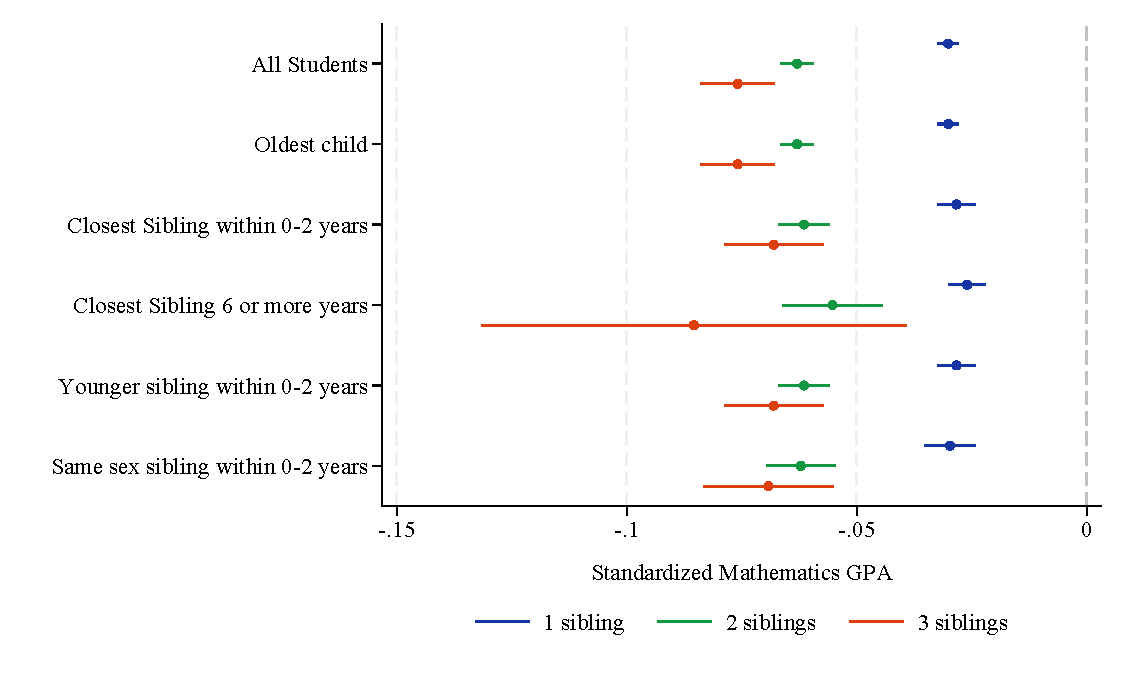
\includegraphics{./FIGURES/TWFE/covid_twfe_C_bysibs_elm_all_gpa_m_adj_Tsiblings_Soldest_4.pdf}
        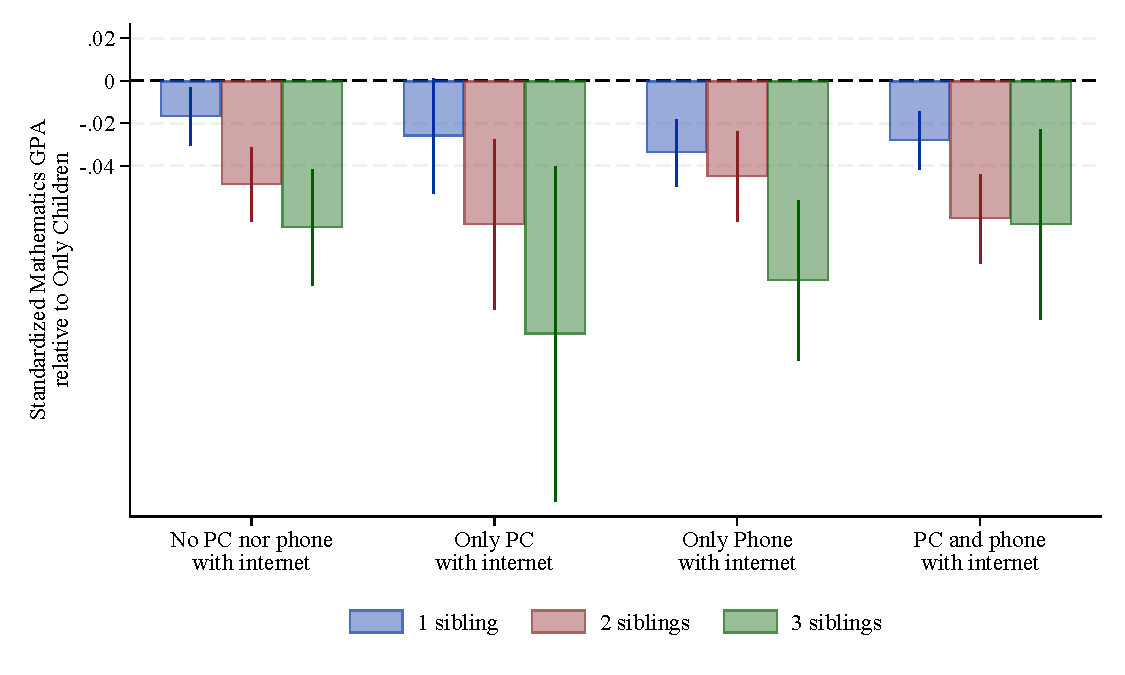
\includegraphics{./FIGURES/TWFE/twfe_std_gpa_m_adj_byresour4_bysibs_Tsiblings_Soldest_pairall_4.pdf}
      }
    }

    \begin{flushleft}
        \hyperlink{frame:resources}{\beamergotobutton{Go Back $\carriagereturn$}}
    \end{flushleft}       

\end{frame}

\begin{frame}
    \label{frame:siblingdisruption_siblings}
    \frametitle{Sibling disruption}
        {\resizebox{0.9\textwidth}{!}{
        %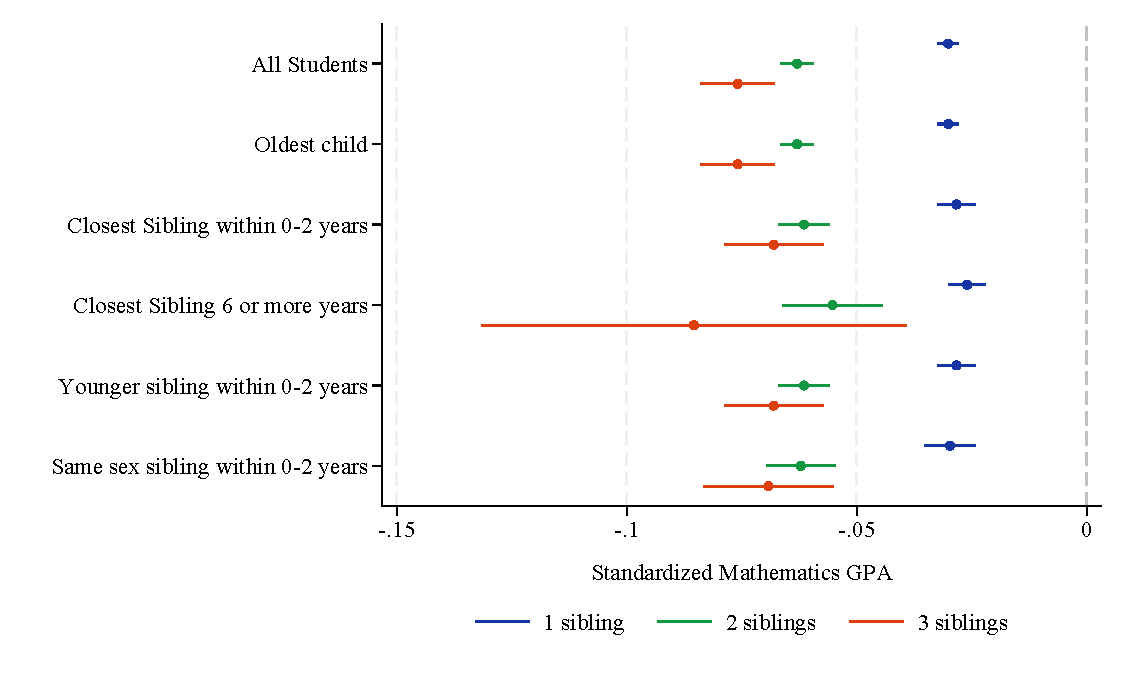
\includegraphics{./FIGURES/TWFE/covid_twfe_C_bysibs_elm_all_gpa_m_adj_Tsiblings_Soldest_4.pdf}
        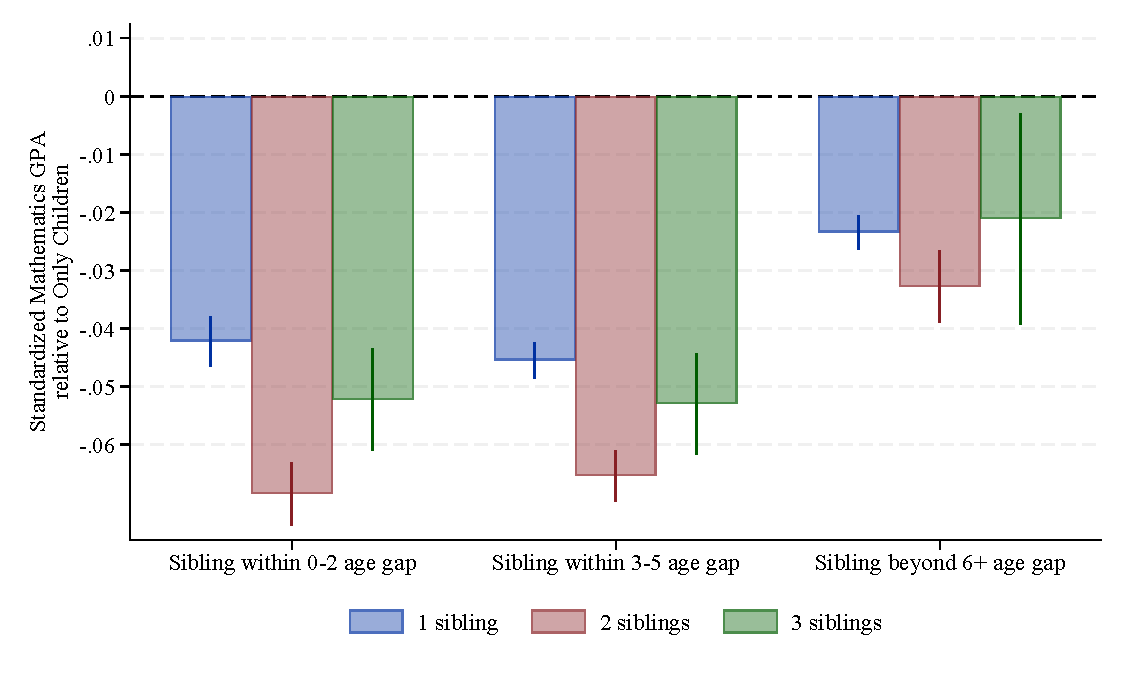
\includegraphics{./FIGURES/TWFE/twfe_gpa_age_gap_bysibs_20_21_Tsiblings_Soldest_4.pdf}
      }
    }

    \begin{flushleft}
        \hyperlink{frame:siblingdisruption}{\beamergotobutton{Go Back $\carriagereturn$}}
    \end{flushleft}        

\end{frame}


\begin{frame}
    \label{frame:mothereduc}
    \frametitle{Mother's Education}
        {\resizebox{0.9\textwidth}{!}{
        %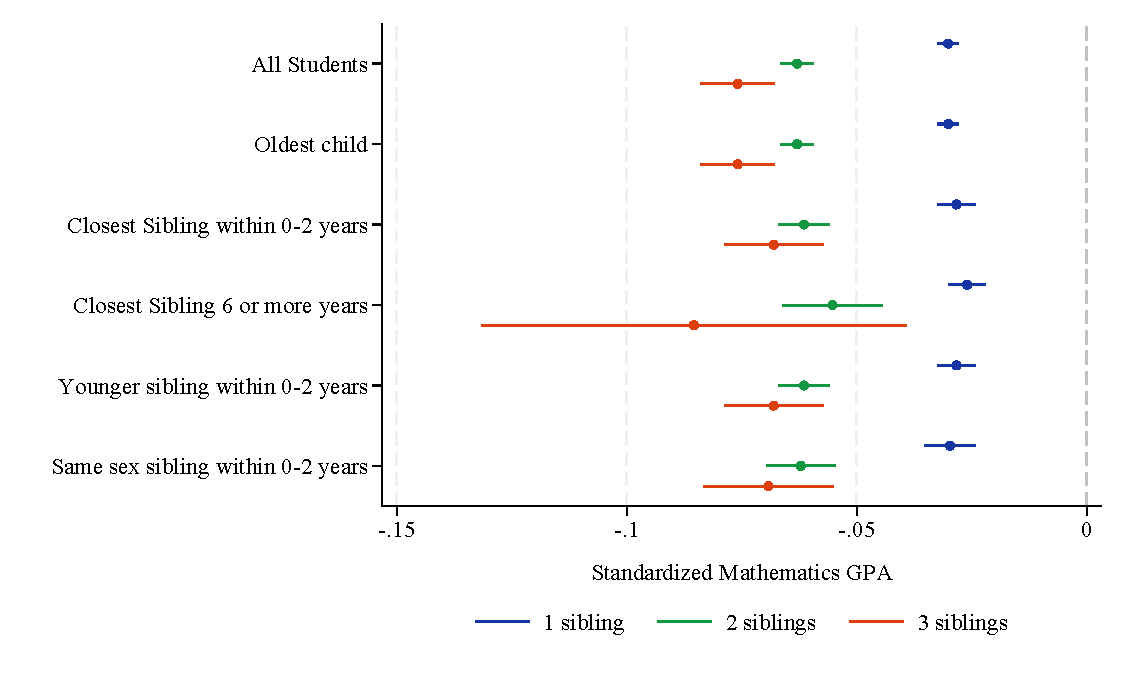
\includegraphics{./FIGURES/TWFE/covid_twfe_C_bysibs_elm_all_gpa_m_adj_Tsiblings_Soldest_4.pdf}
        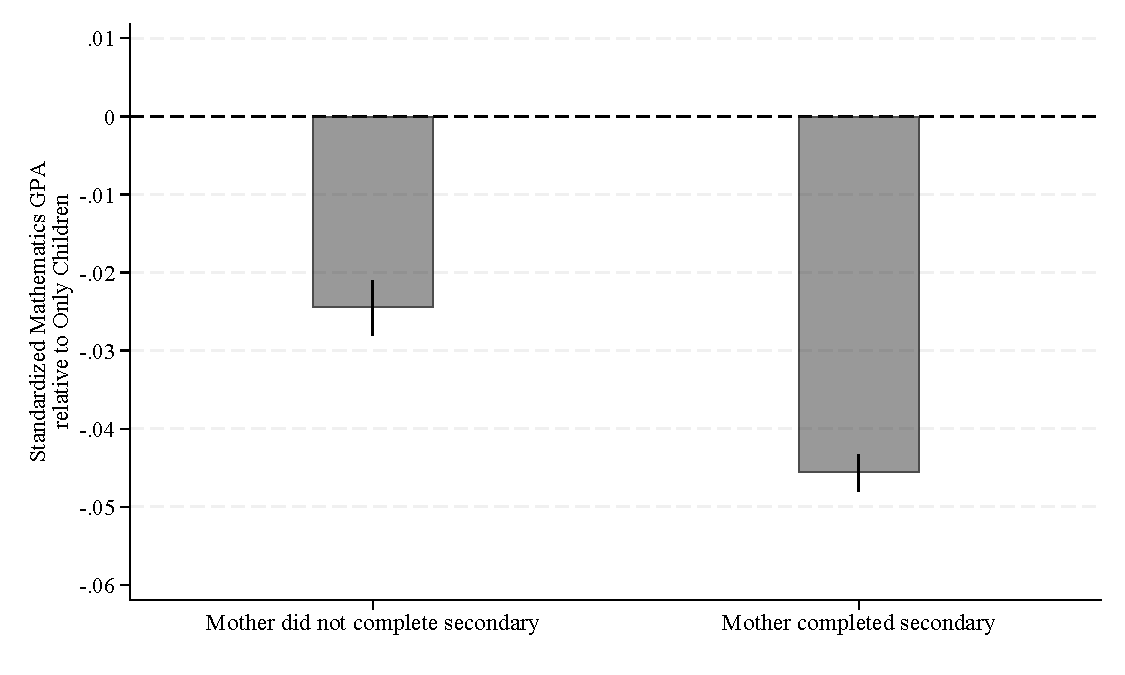
\includegraphics{./FIGURES/TWFE/twfe_gpa_mom_sec_complete_20_21_Tsiblings_Soldest_4.pdf}
      }
    }

    \begin{flushleft}
        \hyperlink{frame:mothereduc_siblings}{\beamergotobutton{Results by siblings}}
    \end{flushleft}    

\end{frame}

\begin{frame}
    \label{frame:mothereduc_siblings}
    \frametitle{Mother's Education}
        {\resizebox{0.9\textwidth}{!}{
        %\includegraphics{./FIGURES/TWFE/covid_twfe_C_bysibs_elm_all_gpa_m_adj_Tsiblings_Soldest_4.pdf}
        \includegraphics{./FIGURES/TWFE/twfe_gpa_mom_sec_complete_bysibs_20_21_Tsiblings_Soldest_4.pdf}
      }
    }

    \begin{flushleft}
        \hyperlink{frame:mothereduc}{\beamergotobutton{Go Back $\carriagereturn$}}
    \end{flushleft}        

\end{frame}


\begin{frame}
    \label{frame:byacad}
    \frametitle{By Academic achievement}
        {\resizebox{0.9\textwidth}{!}{
        %\includegraphics{./FIGURES/TWFE/covid_twfe_C_bysibs_elm_all_gpa_m_adj_Tsiblings_Soldest_4.pdf}
        \includegraphics{./FIGURES/TWFE/twfe_std_gpa_m_adj_byacad_Tsiblings_Soldest_pairall_4.pdf}
      }
    }

    \begin{flushleft}
        \hyperlink{frame:byacad_siblings}{\beamergotobutton{Results by siblings}}
    \end{flushleft}    

\end{frame}

\begin{frame}
    \label{frame:byacad_siblings}
    \frametitle{By Academic achievement}
        {\resizebox{0.9\textwidth}{!}{
        %\includegraphics{./FIGURES/TWFE/covid_twfe_C_bysibs_elm_all_gpa_m_adj_Tsiblings_Soldest_4.pdf}
        \includegraphics{./FIGURES/TWFE/twfe_std_gpa_m_adj_byacad_bysibs_Tsiblings_Soldest_pairall_4.pdf}
      }
    }

    \begin{flushleft}
        \hyperlink{frame:byacad}{\beamergotobutton{Go Back $\carriagereturn$}}
    \end{flushleft}        

\end{frame}


\begin{frame}
    \label{frame:byasp}
    \frametitle{By Education Expectations}
        {\resizebox{0.9\textwidth}{!}{
        %\includegraphics{./FIGURES/TWFE/covid_twfe_C_bysibs_elm_all_gpa_m_adj_Tsiblings_Soldest_4.pdf}
        \includegraphics{./FIGURES/TWFE/twfe_std_gpa_m_adj_byasp_Tsiblings_Soldest_pairall_4.pdf}
      }
    }

    \begin{flushleft}
        \hyperlink{frame:byasp_siblings}{\beamergotobutton{Results by siblings}}
    \end{flushleft}    

\end{frame}

\begin{frame}
    \label{frame:byasp_siblings}
    \frametitle{By Education Expectations}
        {\resizebox{0.9\textwidth}{!}{
        %\includegraphics{./FIGURES/TWFE/covid_twfe_C_bysibs_elm_all_gpa_m_adj_Tsiblings_Soldest_4.pdf}
        \includegraphics{./FIGURES/TWFE/twfe_std_gpa_m_adj_byasp_bysibs_Tsiblings_Soldest_pairall_4.pdf}
      }
    }

    \begin{flushleft}
        \hyperlink{frame:byasp}{\beamergotobutton{Go Back $\carriagereturn$}}
    \end{flushleft}        

\end{frame}


%%%%%%%%%%%%%%%%%%%%%%%%%%%%%%%%%%%%%%%%%%%%%%%%%%%%%
\section{GPA with baseline controls by grade}
%%%%%%%%%%%%%%%%%%%%%%%%%%%%%%%%%%%%%%%%%%%%%%%%%%%%%

\begin{frame}
    \label{frame:twfe_gpa_controls_1}
    \frametitle{6th graders with 2nd grade baseline}
        {\resizebox{0.9\textwidth}{!}{
       %\includegraphics{./FIGURES/TWFE/covid_twfe_summ_bysibs_all_20-21_gpa_m_adj_Tsiblings_Soldest_4.pdf}
       \includegraphics{./FIGURES/TWFE/twfe_std_gpa_m_adj_bycontrols_Tsiblings_Soldest_pair1_4.pdf}
      }
    }

    \begin{flushleft}
        \hyperlink{frame:twfe_gpa_controls}{\beamergotobutton{Go Back $\carriagereturn$}}
    \end{flushleft}       
\end{frame}

\begin{frame}
    \label{frame:twfe_gpa_controls_2}
    \frametitle{6th graders with 4th grade baseline}
        {\resizebox{0.9\textwidth}{!}{
       %\includegraphics{./FIGURES/TWFE/covid_twfe_summ_bysibs_all_20-21_gpa_m_adj_Tsiblings_Soldest_4.pdf}
       \includegraphics{./FIGURES/TWFE/twfe_std_gpa_m_adj_bycontrols_Tsiblings_Soldest_pair2_4.pdf}
      }
    }

    \begin{flushleft}
        \hyperlink{frame:twfe_gpa_controls}{\beamergotobutton{Go Back $\carriagereturn$}}
    \end{flushleft}       
\end{frame}

\begin{frame}
    \label{frame:twfe_gpa_controls_3}
    \frametitle{7th graders with 4th grade baseline}
        {\resizebox{0.9\textwidth}{!}{
       %\includegraphics{./FIGURES/TWFE/covid_twfe_summ_bysibs_all_20-21_gpa_m_adj_Tsiblings_Soldest_4.pdf}
       \includegraphics{./FIGURES/TWFE/twfe_std_gpa_m_adj_bycontrols_Tsiblings_Soldest_pair3_4.pdf}
      }
    }

    \begin{flushleft}
        \hyperlink{frame:twfe_gpa_controls}{\beamergotobutton{Go Back $\carriagereturn$}}
    \end{flushleft}       
\end{frame}

\begin{frame}
    \label{frame:twfe_gpa_controls_4}
    \frametitle{9th graders with 8th grade baseline}
        {\resizebox{0.9\textwidth}{!}{
       %\includegraphics{./FIGURES/TWFE/covid_twfe_summ_bysibs_all_20-21_gpa_m_adj_Tsiblings_Soldest_4.pdf}
       \includegraphics{./FIGURES/TWFE/twfe_std_gpa_m_adj_bycontrols_Tsiblings_Soldest_pair4_4.pdf}
      }
    }

    \begin{flushleft}
        \hyperlink{frame:twfe_gpa_controls}{\beamergotobutton{Go Back $\carriagereturn$}}
    \end{flushleft}       
\end{frame}


\section{Income shock by siblings}


\begin{frame}
    \label{frame:incomeshocks_siblings}
    \frametitle{Income Shocks}
     
    %\makeatletter
\@ifclassloaded{beamer}{%
       \centering
       \resizebox{0.6\textwidth}{!}%
}{%
       \begin{table}[!tbp]\centering\def\sym#1{\ifmmode^{#1}\else\(^{#1}\)\fi}
       \centering
       \caption{TWFE on Standardized Exams, Expectations and Socio-Economic Status}
       \label{tab:twfe_ece}
       \resizebox{0.8\textwidth}{!}%
}
{
\makeatother
\begin{tabular}{lccc}
\toprule
\cmidrule(lr){2-4}
& \multicolumn{3}{c}{TWFE}  \\
\cmidrule(lr){2-4}
& 1 sibling & 2 siblings & 3 siblings  \\
\cmidrule(lr){2-2} \cmidrule(lr){3-3} \cmidrule(lr){4-4}
& (1) & (2) & (3)\\
\bottomrule
&  &  &  \\
&  &  &   \\
\multicolumn{4}{l}{\textit{Panel A: 2nd grade students}} \\
\hspace{3mm}Mathematics&      -0.028** &      -0.090***&      -0.093   \\
                    &     (0.011)   &     (0.023)   &     (0.081)   \\
 
%&  &  &   \\
\hspace{3mm}Reading &      -0.028** &      -0.068***&      -0.140*  \\
                    &     (0.011)   &     (0.022)   &     (0.078)   \\
 
%&  &  &   \\
\hspace{3mm}Max Expectation: Finish school&       0.008***&      -0.002   &      -0.026   \\
                    &     (0.003)   &     (0.006)   &     (0.022)   \\
 
%&  &  &   \\
\hspace{3mm}Max Expectation: 4-year college&      -0.011** &       0.004   &      -0.010   \\
                    &     (0.004)   &     (0.009)   &     (0.034)   \\
 
%&  &  &   \\
\hspace{3mm}SES     &       0.018** &       0.022   &       0.058   \\
                    &     (0.009)   &     (0.019)   &     (0.069)   \\
 
&  &  &   \\
\multicolumn{4}{l}{\textit{Panel B: 4th grade students}} \\
\hspace{3mm}Mathematics&      -0.022***&      -0.103***&      -0.172***\\
                    &     (0.004)   &     (0.008)   &     (0.022)   \\
 
%&  &  &   \\
\hspace{3mm}Reading &      -0.027***&      -0.103***&      -0.139***\\
                    &     (0.004)   &     (0.008)   &     (0.022)   \\
 
%&  &  &   \\
\hspace{3mm}Max Expectation: Finish school&       0.006***&       0.004   &       0.005   \\
                    &     (0.001)   &     (0.003)   &     (0.008)   \\
 
%&  &  &   \\
\hspace{3mm}Max Expectation: 4-year college&      -0.012***&      -0.020***&      -0.032***\\
                    &     (0.002)   &     (0.004)   &     (0.010)   \\
 
%&  &  &   \\
\hspace{3mm}SES     &       0.017***&      -0.005   &       0.004   \\
                    &     (0.003)   &     (0.006)   &     (0.019)   \\
 
&  &  &   \\
\multicolumn{4}{l}{\textit{Panel C: 8th grade students}} \\
\hspace{3mm}Mathematics&      -0.014** &      -0.036***&      -0.029   \\
                    &     (0.007)   &     (0.010)   &     (0.018)   \\
 
%&  &  &   \\
\hspace{3mm}Reading &       0.005   &      -0.009   &      -0.023   \\
                    &     (0.007)   &     (0.009)   &     (0.017)   \\
 
%&  &  &   \\
\hspace{3mm}Max Expectation: Finish school&      -0.011   &      -0.001   &       0.051***\\
                    &     (0.010)   &     (0.013)   &     (0.019)   \\
 
%&  &  &   \\
\hspace{3mm}Max Expectation: 4-year college&      -0.007   &      -0.003   &      -0.054** \\
                    &     (0.014)   &     (0.017)   &     (0.026)   \\
 
%&  &  &   \\
\hspace{3mm}SES     &       0.017***&       0.026***&       0.038***\\
                    &     (0.005)   &     (0.008)   &     (0.014)   \\
 

\bottomrule
\end{tabular}
}
\@ifclassloaded{beamer}{%
}{%
       \end{table}
}


     {\resizebox{0.9\textwidth}{!}{
        \includegraphics{./FIGURES/TWFE/twfe_ses_bysibs_2_4_Tsiblings_Soldest_4.pdf}
      }
    }

 \begin{flushleft}
        \hyperlink{frame:incomeshocks}{\beamergotobutton{Go Back $\carriagereturn$}}
    \end{flushleft}   
    
    
\end{frame}

%
%####
%%%%%%%%%%%%%%%%%%%%%%%%%%%%%%%%%%%%%%%%%%%%%%%%%%%%%
\section{Potential concerns}
%%%%%%%%%%%%%%%%%%%%%%%%%%%%%%%%%%%%%%%%%%%%%%%%%%%%%



% ========================================
% Some thoughts
% ========================================

\section{Thoughts}

\begin{frame}
    \label{frame:thoughts}
    \frametitle{Thoughts}
    \begin{itemize}
        \item How to think about heterogeneity? We should expect more effects not where there lacks parental suppport but where there is $\rightarrow$ more possibilities of substitution from teachers to parents. But not too much because otherwise they could do it all?
        \item Have school level estimates. Idea was to do heterogeneity. Needed or our excercise is enough?
    \end{itemize}


\end{frame}


\begin{frame}
    \label{frame:research_feedback}
    \frametitle{Threats to identification \textcolor{red}{(for feedback)}}
        Any other thoughts on potential time varying shocks?
        \begin{itemize}
            \item Parent's work
            \item 
            \item There is a shift from private to public enrollment during COVID. If this was more common on siblings... would be composition?
        \end{itemize}

 
    \begin{flushleft}
        \hyperlink{frame:research}{\beamergotobutton{Go Back $\carriagereturn$}}
    \end{flushleft}
    
\end{frame}


\begin{frame}
        \label{frame:Leigh}
    \frametitle{Leigh}
    \begin{itemize}
        \item 
    \end{itemize}
\end{frame}

\begin{frame}
        \label{frame:Scott}
    \frametitle{Scott}
    \begin{itemize}
        \item 
    \end{itemize}
\end{frame}

\begin{frame}
        \label{frame:Rich}
    \frametitle{Rich}
    \begin{itemize}
        \item 
    \end{itemize}
\end{frame}


\begin{frame}
        \label{frame:dean}
    \frametitle{Dean}
    \begin{itemize}
        \item \textbf{Sibsize is not exogenou.}  Sibsize is correlated with parents age (sibsize unfolds over a lifecycle), parents age at first birth, parents employment, parents human capital, housing choices, etc. How much should we really be interpreting this as about sibsize? What if there are two types of parents, those who really care about investing in child quality (H) and human capital and those who do not (L). H types choose to have smaller sibsize so they can invest more in human capital, L types choose quantity over quality. AND when covid comes H types sacrifice more to protect learning than L types do. So you’re not identifying an effect of sibsize; you’re recovering the parents’ endogenous choices that determined sibsize.
    \end{itemize}
\end{frame}

\begin{frame}
        \label{frame:dean2}
    \frametitle{Dean}
    \begin{itemize}
        \item \textbf{Measurement of the dependent variable.}   How is the outcome measured? GPAs seem like they could be directly impacted by covid in ways that are about measurement rather than education. Like, you’re not going to school in the same way, so you’re not being evaluated the same way. I understand that this would be presumably constant by sibship size, but it seems like at a minimum it bears on the interpretation of the results and whether they have a quantitative (rather than just qualitative) interpretation. (It also gets me wondering about strict exogeneity (assuming that you’re using period fixed effects) and the linearity assumptions built into fixed effects.)
    \end{itemize}
\end{frame}

\begin{frame}
        \label{frame:dean3}
    \frametitle{Dean}
    \begin{itemize}
        \item \textbf{Is the effect size quantitatively informative?}   A JMP has to be interesting to get attention. I don’t know that people are going to be super-surprised by the sign of the effect. So is the effect size stably robust, interesting and informative?
    \end{itemize}
\end{frame}

\begin{frame}
        \label{frame:Eric}
    \frametitle{Eric}
    \begin{itemize}
        \item 
    \end{itemize}
\end{frame}

\begin{frame}
        \label{frame:Sandy}
    \frametitle{Sandy}
    \begin{itemize}
        \item 
    \end{itemize}
\end{frame}

\begin{frame}
        \label{frame:Bo}
    \frametitle{Bo}
    \begin{itemize}
        \item 
    \end{itemize}
\end{frame}

\begin{frame}
        \label{frame:Peter}
    \frametitle{Peter}
    \begin{itemize}
        \item 
    \end{itemize}
\end{frame}

\begin{frame}
        \label{frame:Ofer}
    \frametitle{Ofer}
    \begin{itemize}
        \item 
    \end{itemize}
\end{frame}

\begin{frame}
    \label{frame:fabiola}
    \frametitle{Fabiola}
    \begin{itemize}
        \item 
    \end{itemize}
\end{frame}


\end{document}